%%%% File:           lmsthesis.tex
%%%% Created:        2015-08-20
%%%% Modified:       2015-10-05
%%%% Author:         Dipl.-Ing. Marcus Laumer
%%%% Description:    This LaTeX template is supposed to be used for writing a thesis at the chair of
%%%%                 Multimedia Communications and Signal Processing (LMS) at the Friedrich-Alexander-Universität Erlangen-Nürnberg (FAU)

\documentclass[
paper=A4,               % paper format
pagesize=auto,          % provide page size for compiler
fontsize=12pt,          % font size
DIV=16,                 % type area calculation
twoside=true,           % two-sided layout for printing
BCOR=20mm,              % binding correction for printing (ask at copy shop!)
parskip=false,          % space between paragraphs
chapterprefix=true,     % prefix before chapter names: Chapter #
appendixprefix=true,    % prefix before appendix names: Appendix #
listof=totoc,           % include lists of figures and tables in TOC
bibliography=totoc,     % include bibliography in TOC
headinclude=true,       % header included in type area
footinclude=false,      % footer included in type area
headsepline=true,       % separation line between header and text
footsepline=false,      % separation line between footer and text
headings=small,         % size of headings
numbers=noenddot        % no dot after chapter heading prefixes
] {scrbook}

\usepackage{lmodern}
\usepackage[T1]{fontenc}
\usepackage[utf8]{inputenc}
%\usepackage[ngerman]{babel} % can be used for writing the thesis in German
\usepackage[onehalfspacing]{setspace}
\usepackage{amsmath,amssymb}
\usepackage{graphicx}
\usepackage{wrapfig}
\usepackage[caption=false]{subfig}
\usepackage{booktabs}
\usepackage[printonlyused]{acronym}
\usepackage{pdfpages}

\usepackage{blindtext} % delete in final version!

% custom packages
\usepackage[backref=page]{hyperref}
% for backreference with arrow
\renewcommand\backrefxxx[3]{%
  \hyperlink{page.#1}{$\uparrow$#1}%
}
% better than actronym package, makes them auto alphabetically sorted
\usepackage[toc]{glossaries}

\graphicspath{{../images/}{../images/analyze/}}

\recalctypearea

% define acronyms, need to be in preamble
% old version of acronyms.tex
% \chapter{Abbreviations and Acronyms}

% In alphabetical order.

% \begin{acronym}
%     \acro{e.g.}{exempli gratia}
%     \acro{TER}{text error rate}
%     \acro{MOS}{mean opinion score}
% \end{acronym}

\newacronym{ocr}{OCR}{optical character recognition}
\newacronym{cer}{CER}{character error rate}
\newacronym{mos}{MOS}{mean opinion score}
\newacronym{psnr}{PSNR}{peak signal-to-noise ratio}
\newacronym{mse}{MSE}{mean squared error}
\newacronym{bdrate}{BDRate}{Bjøntegaard Delta Rate}
\newacronym{hevc}{HEVC}{High Efficiency Video Coding}
\newacronym{vvc}{VVC}{Versatile Video Coding}
\newacronym{scid}{SCID}{Screen Content Image Database}
\newacronym{gt}{GT}{ground truth}


\begin{document}

    \pagenumbering{Alph} % will not be displayed
    \begin{titlepage}
    \vspace*{6ex}
    \begin{center}
        \LARGE
        Friedrich-Alexander-Universität Erlangen-Nürnberg\\[1.5ex]
        \Large
        \textbf{Lehrstuhl für Multimediakommunikation und Signalverarbeitung}\\[1.5ex]
        Prof. Dr.-Ing. André Kaup\\
        \vfill
        \LARGE
        Master Thesis\\[3ex]
        \textbf{Text Recognition Algorithms for Screen Content Quality Assessment}\\[3ex]
        Sebastian Hirt\\
        \vfill
        \Large
        July 2023\\[1.5ex]
        \begin{tabular}{ll}
            Supervisors: & Prof. Dr.-Ing. André Kaup \\
            & M. Sc. Hannah Och
        \end{tabular}
    \end{center}
\end{titlepage}

    \cleardoublepage
    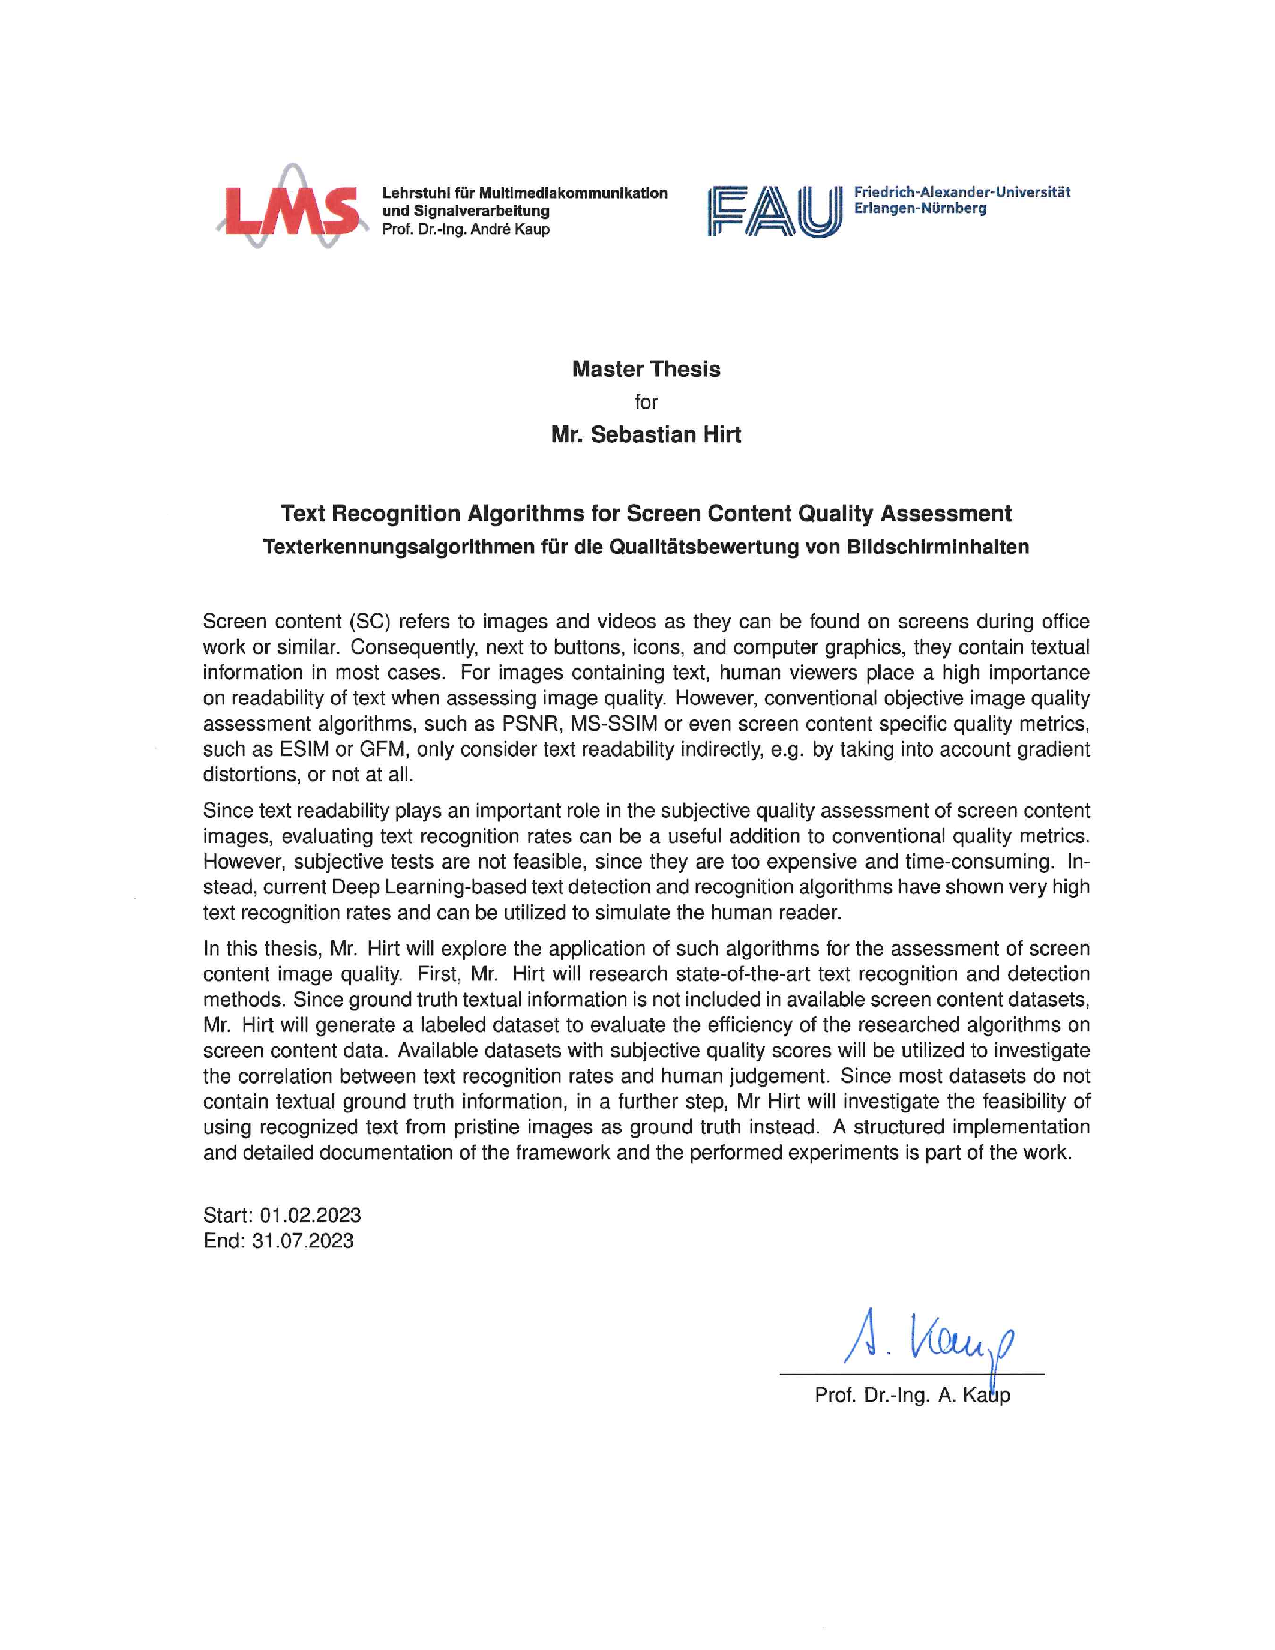
\includepdf[pages={1},scale={0.95}]{../organizing/MA_AufgabenstellungUnterzeichnet_searchable.pdf}
    \cleardoublepage
    
    %\chapter*{Erklärung}
\thispagestyle{empty}

\noindent
Ich versichere, dass ich die vorliegende Arbeit ohne fremde Hilfe und ohne Benutzung anderer als der angegebenen Quellen angefertigt habe, und dass die Arbeit in gleicher oder ähnlicher Form noch keiner anderen Prüfungsbehörde vorgelegen hat und von dieser als Teil einer Prüfungsleistung angenommen wurde.
Alle Ausführungen, die wörtlich oder sinngemäß übernommen wurden, sind als solche gekennzeichnet.

\vspace{3cm}

\begin{minipage}[t]{0.45\textwidth}
    \rule{\textwidth}{0.5pt}\\
	Ort, Datum
\end{minipage}
\hfill
\begin{minipage}[t]{0.45\textwidth}
	\rule{\textwidth}{0.5pt}\\
	<Vollständiger Name>\\
    <Adresse>
\end{minipage}

    % or
    \chapter*{Declaration}
\thispagestyle{empty}

\noindent
I confirm that I have written this thesis unaided and without using sources other than those listed and that this thesis has never been submitted to another examination authority and accepted as part of an examination achievement, neither in this form nor in a similar form.
All content that was taken from a third party either verbatim or in substance has been acknowledged as such.

\vspace{3cm}

\begin{minipage}[t]{0.45\textwidth}
    \rule{\textwidth}{0.5pt}\\
	Erlangen, \today
\end{minipage}
\hfill
\begin{minipage}[t]{0.45\textwidth}
	\rule{\textwidth}{0.5pt}\\
	Sebastian Hirt\\
    Ellingen, Rennfeld 5b
\end{minipage}


    \frontmatter
    \pagenumbering{Roman}
    \tableofcontents
    \chapter{Kurzfassung}

In dieser Arbeit wird die Anwendung von Texterkennungsalgorithmen für die Bewertung der Bildqualität von Bildschirminhalten untersucht.
Durch die Untersuchung modernster Texterkennungs- und -erkennungsmethoden, die Erstellung eines markierten Datensatzes und die Untersuchung der Korrelation zwischen Texterkennungsraten und menschlicher Beurteilung wird eine wertvolle Ergänzung zur aktuellen Forschung geliefert.

    \chapter{Abstract}

In this thesis, the application of text recognition algorithms for the assessment of screen content image quality is explored.
By researching state-of-the-art text recognition and detection methods, generating a labeled dataset, and investigating the correlation between text recognition rates and human judgement, a valuable addition to current research is provided.

    % \chapter{Symbols and Notations}

% In order of appearance.\\

% \begin{tabular}{ll}
% +					&	Addition\\
% \end{tabular}
% \makenoidxglossaries

\newglossaryentry{add}
{
    type={symbols},
    name={+},
    description={Addition}
}

\newglossaryentry{sub}
{
    type={symbols},
    name={-},
    description={Subtraction}
}


    % glossary, makes them auto alphabetically sorted
    \printnoidxglossary[title=Abbreviations and Acronyms]

    \mainmatter
    \chapter{Introduction}
\label{chap:Introduction}

\section{Motivation}

In today’s digital age, screen content plays a vital role in our daily lives.
From office work to entertainment, we are constantly interacting with images and videos on screens.
Many of these images contain text, graphics and user interface elements that are not found in natural images.
As such, the quality of screen content is of utmost importance for the viewer.
One key aspect of screen content quality is the readability of text.
However, conventional objective image quality assessment algorithms do not directly consider text readability.
This is where text recognition algorithms come into play.

In this thesis, we will explore the application of text recognition algorithms for the assessment of screen content image quality.
By researching state-of-the-art text recognition and detection methods, generating a labeled dataset, and investigating the correlation between text recognition rates and human judgement, we aim to provide a valuable addition to conventional quality metrics.

Through a structured implementation and detailed documentation of the framework and experiments, this thesis will provide valuable insights into the potential of text recognition algorithms for screen content quality assessment.
In this thesis, I use the pronouns \textit{we} and \textit{our} to refer to myself and the larger scientific community.

\section{Research Objectives}

--- Figure out if text recognition algorithms can be used to assess the quality of screen content images.

\section{Thesis Outline}

--- do this last

First we will give an overview of the current state of the art in text recognition and detection in \autoref{chap:related_work}.
Then we will describe the methodology used in this thesis in \autoref{chap:methods}.
Afterwards, we will present the results of our experiments in \autoref{chap:evaluation}.
Finally, we will summarize and conclude our findings in \autoref{chap:conclusion}.

    \chapter{Methods}
\label{chap:methods}

In this chapter, the methods used in this thesis are described.

\section{Optical Character Recognition}
\label{sec:ocr}

In this section, the \gls{ocr} methods used in this thesis are described.

\subsection{EasyOCR}
\label{subsec:easyocr}

EasyOCR is a Python library for \gls{ocr} \cite{easyocr_2020}. It uses a deep learning model to detect text.

\subsection{Tesseract}
\label{subsec:tesseract}

Tesseract is an \gls{ocr} engine \cite{tesseract_2007}. It is open-source and was developed by Google. It is written in C++ and has a Python wrapper.

\subsection{Other Optical Character Recognition Methods}
\label{subsec:other_ocr_methods}

We don't use other \gls{ocr} methods in this thesis.
However, we mention them here for completeness.


\section{Metrics}
\label{sec:metrics}

In this section, we go over the metrics used in this thesis.

\subsection{Character Error Rate}
\label{subsec:cer}

The \gls{cer} is defined as follows:

\begin{equation}
    \text{CER} = \frac{S + D + I}{N}
    \label{eq:cer}
\end{equation}
with \(S\) being the number of substitutions, \(D\) the number of deletions, \(I\) the number of insertions, and \(N\) the total number of characters of the label.
The \gls{cer} ranges from 0 to $\infty$, where 0 means perfect recognition and the higher the worse the recognition.
Because the \gls{mos} is defined in the range 0 to 100 and 100 represents a high subjective quality, the two metrics are unintuitive to compare.
Therefore, transform the CER by subtracting it from 1 and multiplying it by 100 to get a \gls{mos}-like value, see \autoref{eq:cer2mos}.
\begin{equation}
    \text{CER} = (1 - \text{TER}_{raw}) \cdot 100.
    \label{eq:cer2mos}
\end{equation}

\subsection{Peak Signal-to-Noise Ratio}
\label{subsec:psnr}

The \gls{psnr} is defined as follows:

\begin{equation}
    \text{PSNR} = 10 \cdot \log_{10} \left( \frac{R^2}{\text{MSE}} \right)
    \label{eq:psnr}
\end{equation}

with \(R\) being the maximum possible pixel value of the image and \gls{mse} being the mean squared error between the original and the reconstructed image.

\subsection{Bjøntegaard Delta Rate}
\label{subsec:bdrate}

The \gls{bdrate} is defined by the difference between the integration of curves of the codecs to compare. The first curve is the reference curve and the second the test curve. Both are plotting some average metric over the average bitrate of some images.

\begin{equation}
    \text{BDRate} = https://arxiv.org/pdf/2202.12565.pdf
    \label{eq:bdrate}
\end{equation}

\section{Codecs}
\label{sec:codecs}

In this section, the codecs used in this thesis are described.

\subsection{High Efficiency Video Coding}
\label{subsec:hevc}

\gls{hevc} is a video codec.

\subsection{Versatile Video Coding}
\label{subsec:vvc}

\gls{vvc} is a video codec.

\section{Nonlinear Transformation}
\label{sec:nonlinear}

In this section, we describe the nonlinear transformation used to tranform the \gls{mos} to better fit the \gls{cer}.
The transformation is defined as follows:

\begin{equation}
    \text{MOS}_{trans} = \frac{a - b}{1 + \exp \left( \frac{-\text{MOS} + c}{d} \right)} + b
    \label{eq:nonlinear}
\end{equation}
    
We fit the parameters \(a\), \(b\), \(c\), and \(d\) to the data of all the test images. We then fit use the function to transform the MOS into the $\text{MOS}_{trans}$.

    \chapter{Dataset}
\label{chap:dataset}
In this chapter, we present the dataset used in our work.
We use the \gls{scid} dataset \cite{ni_esim_2017}\footnote{The dataset can be downloaded here: https://eezkni.github.io/publications/ESIM.html.} as the base for our experiments.
The \gls{scid} dataset is suitable for our work, since the images contain text on \glspl{sci}, different distortion levels and \gls{mos} values for each image.
Among the available screen content datasets mentioned in the literature \cite{iqa_survey_2020}, we find that other options are either inaccessible or fail to fulfill all the necessary criteria we require for our research.
An overview of the 40 reference images of the \gls{scid} dataset can be seen in \autoref{fig:dataset_overview}.
Additionally, the dataset contains 1800 distorted images, which we discuss in the next section in detail.
Further, \gls{mos} values are included for each of the distorted images, which represent the perceived quality by a human observer.
The subjective tests to obtain the \gls{mos} values were conducted using the double stimulus method, involving the following steps.
First, the reference image was shown to the candidates for 10 seconds, followed by a mid-gray screen.
Afterwards, the distorted image was shown for 10 seconds.
Finally, the candidates were asked to rate the distorted image's quality compared to the reference image on a 5-point scale, 1 being the worst and 5 being the best.
These scores are then converted to a \gls{mos} value for each image between 0 and 100, with 100 representing the highest quality.
\begin{figure}
    \centering
    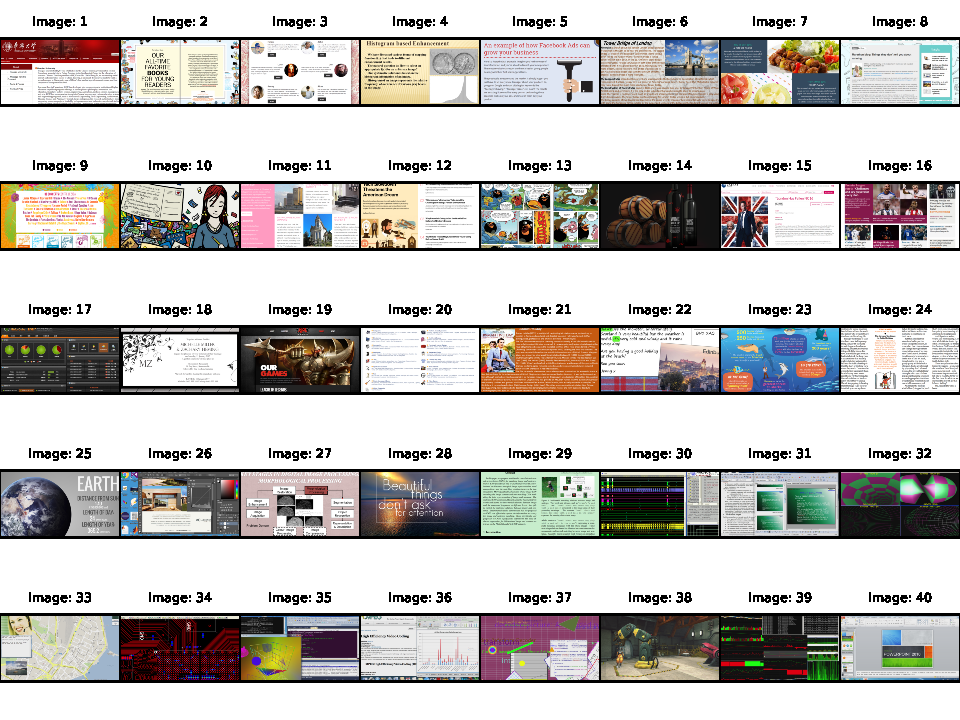
\includegraphics[width=\textwidth]{reference_images}
    \caption{The 40 references images of the dataset.}
    \label{fig:dataset_overview}
\end{figure}


\section{Distortion types}
\label{sec:dataset_distortion_types}


The 1800 distorted images are generated from the 40 reference images \cite{ni_esim_2017}.
They are distorted with 9 different distortion types, each with 5 different distortion quality levels.
In \autoref{tab:distortion_types}, we list the distortion types with a short description.
\begin{table}
\centering
\caption{Overview of the distortion types used in the dataset.}
\begin{tabular}{|p{6cm}|c|p{6cm}|}
\hline
\textbf{Distortion Type} & \textbf{Abbreviation} & \textbf{Description} \\
\hline
\hline
Gaussian Noise & GN & Addition of noise to an image using a Gaussian distribution \\
\hline
Gaussian Blur & GB & Blurring of an image using a Gaussian kernel \\
\hline
Motion Blur & MB & Blurring of an image due to movement of the camera or the object \\
\hline
Contrast Change & CC & Change in the contrast of an image \\
\hline
Joint Photographic Experts Group & JPEG & Image compression standard \\
\hline
Joint Photographic Experts Group 2000 & JPEG2000 & Image compression standard \\
\hline
Color Saturation Change & CSC & Changes in the color saturation of an image \\
\hline
High Efficiency Video Coding-Screen Content Coding & HEVC-SCC & Video compression standard for screen content \\
\hline
Color Quantization with Dithering & CQD & Reduction of colors available in an image \\
\hline
\end{tabular}
\label{tab:distortion_types}
\end{table}
The images distorted by \gls{gn} have noise added with zero mean and standard deviations of $0.001$, $0.005$, $0.01$, $0.05$ and $0.1$ for each quality level, respectively.
The images distorted by \gls{gb} are blurred with a Gaussian kernel.
The size of the kernel is $5\times5$ with standard deviations of $0.58$, $0.76$, $0.96$, $1.2$ and $2.1$ for each quality level, respectively.
Images distorted by \gls{mb} are blurred with a motion kernel, which simulates motion blur.
The parameter, which controls the degree of angle in a counter-clockwise direction, is set to zero and the parameter, which determines the length of the movement of the simulated camera, is set to $2$, $3.4$, $4$, $5.5$ and $6.4$, respectively.
The \gls{cc} distortion scales certain pixel values in the reference image to new values to change the contrast.
The scaling is applied for the ranges $[0,1] \rightarrow [0.3,0.5]$, $[0,1] \rightarrow [0.1,0.7]$, $[0.1,0.8] \rightarrow [0.1,0.9]$, $[0.2,0.8] \rightarrow [0.1,0.8]$ and $[0.2,0.7] \rightarrow [0,1]$, respectively.
So for the first quality level, all pixel values (from 0 to 1) are scaled to values between 0.3 and 0.5 of the maximum pixel intensity.
For the \gls{jpeg} compression, the images are compressed by the image compression algorithm with quality factors $75$, $35$, $18$, $8$ and $5$, respectively.
The \gls{jpeg}2000 compression is applied with compression ratios of $0.08$, $0.045$, $0.02$, $0.015$ and $0.01$, respectively.
The \gls{csc} distortion keeps the luminance component of the images constant, but scales the chrominance components by the factors $0.96$, $0.72$, $0.58$, $0.42$ and $0.1$, respectively.
The \gls{hevc}-SCC distortion is applied by using the \gls{hevc} codec with the \gls{scc} configuration on the images with the \glspl{qp} set to $16$, $36$, $40$, $42$ and $48$, respectively.
We are unsure which exact software version was used for the \gls{hevc}-\gls{scc} encoding.
The \gls{cqd} distortion is applied by reducing the number of colors available in the image to $30$, $28$, $25$, $10$ and $5$, respectively.
More detailed descriptions of the implementation of the distortions can be found in the supporting file included with the dataset.
The different distortion types, at their most severe quality level, can be seen in \autoref{fig:distortion_types}, applied to the image in \autoref{fig:img29}.

\begin{figure}
    \centering
    \includegraphics[width=0.7\textwidth]{../../data/raw/scid/ReferenceSCIs/SCI29.png}
    \caption{Reference image SCI29}
    \label{fig:img29}
\end{figure}

\begin{figure}
    \centering
    \begin{subfigure}[b]{0.42\textwidth}
        \includegraphics[width=\textwidth]{../../data/raw/scid/DistortedSCIs/SCI29_1_5.png}
        \caption{Gaussian Noise}
        \label{fig:distortion_type_1}
    \end{subfigure}
    \hfill
    \begin{subfigure}[b]{0.42\textwidth}
        \includegraphics[width=\textwidth]{../../data/raw/scid/DistortedSCIs/SCI29_2_5.png}
        \caption{Gaussian Blur}
        \label{fig:distortion_type_2}
    \end{subfigure}
    \newline
    \begin{subfigure}[b]{0.42\textwidth}
        \includegraphics[width=\textwidth]{../../data/raw/scid/DistortedSCIs/SCI29_3_5.png}
        \caption{Motion Blur}
        \label{fig:distortion_type_3}
    \end{subfigure}
    \hfill
    \begin{subfigure}[b]{0.42\textwidth}
        \includegraphics[width=\textwidth]{../../data/raw/scid/DistortedSCIs/SCI29_4_5.png}
        \caption{Contrast Change}
        \label{fig:distortion_type_4}
    \end{subfigure}
    \newline
    \begin{subfigure}[b]{0.42\textwidth}
        \includegraphics[width=\textwidth]{../../data/raw/scid/DistortedSCIs/SCI29_5_5.png}
        \caption{JPEG Compression}
        \label{fig:distortion_type_5}
    \end{subfigure}
    \hfill
    \begin{subfigure}[b]{0.42\textwidth}
        \includegraphics[width=\textwidth]{../../data/raw/scid/DistortedSCIs/SCI29_6_5.png}
        \caption{JPEG2000 Compression}
        \label{fig:distortion_type_6}
    \end{subfigure}
    \newline
    \begin{subfigure}[b]{0.42\textwidth}
        \includegraphics[width=\textwidth]{../../data/raw/scid/DistortedSCIs/SCI29_7_5.png}
        \caption{Color Saturation Change}
        \label{fig:distortion_type_7}
    \end{subfigure}
    \hfill
    \begin{subfigure}[b]{0.42\textwidth}
        \includegraphics[width=\textwidth]{../../data/raw/scid/DistortedSCIs/SCI29_8_5.png}
        \caption{HEVC Screen Content Coding}
        \label{fig:distortion_type_8}
    \end{subfigure}
    \newline
    \begin{subfigure}[b]{0.42\textwidth}
        \includegraphics[width=\textwidth]{../../data/raw/scid/DistortedSCIs/SCI29_9_5.png}
        \caption{Color Quantization with Dithering}
        \label{fig:distortion_type_9}
    \end{subfigure}
    \caption{SCI 29 distorted by 9 different distortion types at the most severe level.}
    \label{fig:distortion_types}
\end{figure}

The impact of different distortion types on text within an image is evident.
Among the various distortions, alterations in contrast or color have minimal effect on text legibility for human readers.
Conversely, distortions such as \gls{gn}, \gls{gb} and \gls{mb} can render the text completely unreadable to the human eye.
We might expect that the distortions that affect the text for the human visual system the most, will also affect the \gls{ocr} the most.
It is to note, that all distortions are monotonically decreasing in their severity with the quality level\footnote{It should be noted that referring to it as "quality level" might be somewhat counterintuitive, as the highest "quality level" (level 5) corresponds to the worst quality of the distorted image.} from 1 to 5.
The only exception is \gls{cc}.
As illustrated in \autoref{fig:cc_levels}, \gls{cc} does not display a clear pattern of variation from low contrast to high contrast, or any similar trend.
Understanding this behavior is important for the analysis of the trends of the \gls{mos} over the different quality levels.

\begin{figure}
    \centering
    \begin{subfigure}[b]{0.18\textwidth}
        \includegraphics[width=\textwidth]{../../data/raw/scid/DistortedSCIs/SCI01_4_1.png}
    \end{subfigure}
    \hfill
    \begin{subfigure}[b]{0.18\textwidth}
        \includegraphics[width=\textwidth]{../../data/raw/scid/DistortedSCIs/SCI01_4_2.png}
    \end{subfigure}
    \hfill
    \begin{subfigure}[b]{0.18\textwidth}
        \includegraphics[width=\textwidth]{../../data/raw/scid/DistortedSCIs/SCI01_4_3.png}
    \end{subfigure}
    \hfill
    \begin{subfigure}[b]{0.18\textwidth}
        \includegraphics[width=\textwidth]{../../data/raw/scid/DistortedSCIs/SCI01_4_4.png}
    \end{subfigure}
    \hfill
    \begin{subfigure}[b]{0.18\textwidth}
        \includegraphics[width=\textwidth]{../../data/raw/scid/DistortedSCIs/SCI01_4_5.png}
    \end{subfigure}
    \caption{Distorted image 1 with different levels of \gls{cc}, quality levels from left to right: 1, 2, 3, 4, 5.}
    \label{fig:cc_levels}
\end{figure}

\section{Labeling}
\label{sec:dataset_labeling}

Since we want to evaluate the \gls{ocr} algorithms on theses images, we need a true \gls{gt} in the form of a text label for each image, which are not contained in the dataset \cite{ni_esim_2017}.
The following procedure is used to create the true \gls{gt} for each image.
We start by locating the topmost word in the image.
Then, we identify if this word is part of a line.
If it is, we record the text of the entire line.
Afterwards, we move to the next line or word and repeat the process until all text elements are recorded.
Finally, we combine all the recorded text elements into the full true \gls{gt} by separating them with spaces.
In this process, we ignore paragraphs and only consider the vertical position of the lines.
This true \gls{gt} aligns with the prediction order of the \gls{ocr} algorithms, as discussed in \autoref{subsec:tesseract}.
To avoid introducing bias towards any specific \gls{ocr} algorithm regarding the order of text elements, we made the decision not to utilize one of the algorithms for predicting the text and then correcting it to create the true \gls{gt}, but fully label them ourself.

% --- In ground truth margins of what is in the same line are way slimmer.

% --- The important thing is however that both algorithms have similar rules, so that they can be compared fairly.

\section{Analysis}
\label{sec:dataset_analysis}


Before we continue with our main experiments, we give a short analysis of the dataset.
First, we select a subset of images for our experiments.
Some of the images contain no text at all or only numbers.
Others contain some text, but have a large focus on graphical objects besides the text.
This makes them less suitable for a comparison between the $\text{CER}_{\text{c}}$, which evaluates text, with the \gls{mos}, which evaluates the whole image.
Due to these factors, for our experiments that involve the \gls{mos}, we select the images with
\begin{equation}
    i \in \{1, 2, 3, 4, 5, 6, 7, 8, 11, 12, 15, 18, 20, 21, 24, 29\},
    \label{eq:mos_images}
\end{equation}
as their main focus lies on text elements, instead of graphical objects.
This selection process is subjective, so it might be more reasonable to use all images and filter out outliers later.
Additionally, even if an image only has one small text element, the $\text{CER}_{\text{c}}$ might still be a good estimation of the \gls{mos}, if the distortion affects the text in the same way as the rest of the image.
This however, is not the case for certain distortions, like \gls{jpeg} or other compression algorithms.

\begin{figure}
    \begin{subfigure}[b]{0.45\textwidth}
        \centering
        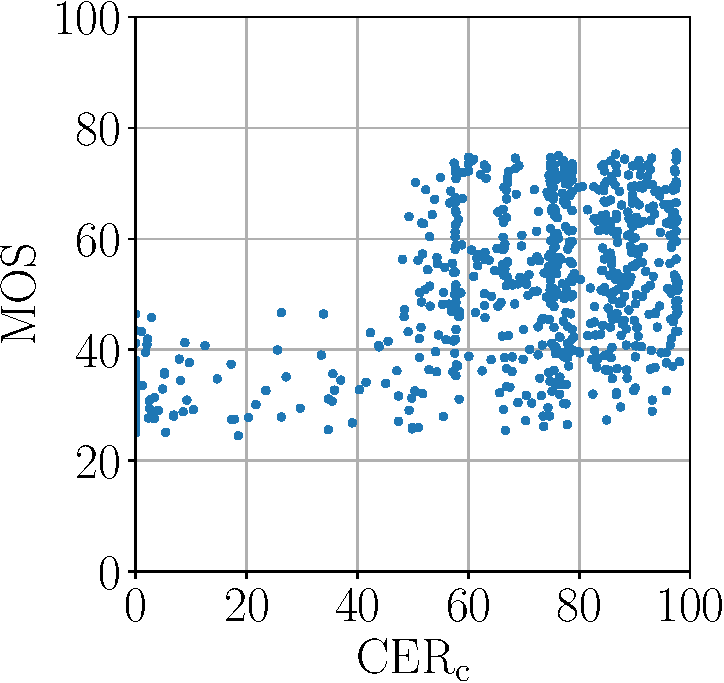
\includegraphics[width=\textwidth]{../../images/cer_mos_overview_gt_tess.pdf}
        \caption{CER vs MOS for Tesseract \gls{ocr} and the true \gls{gt}.}
        \label{fig:cer_vs_mos_gt_tess}
    \end{subfigure}
    \hfill
    \begin{subfigure}[b]{0.45\textwidth}
        \centering
        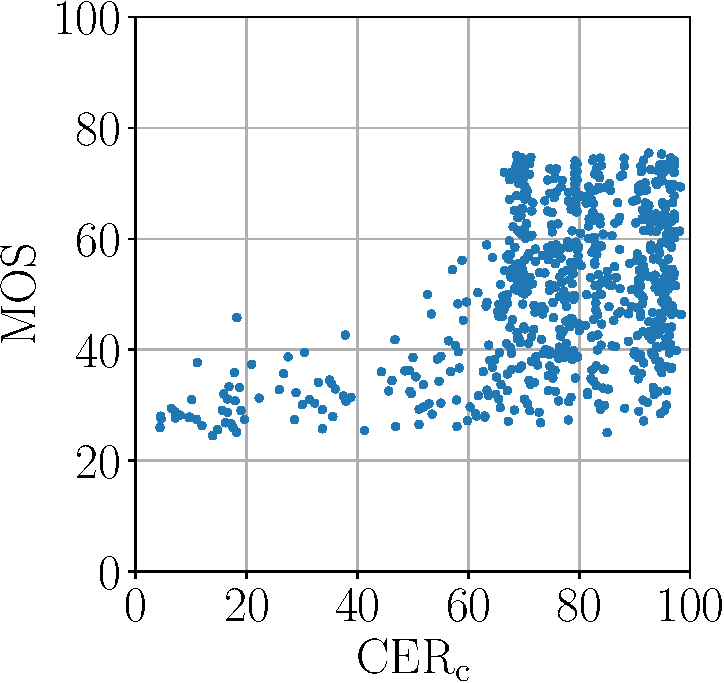
\includegraphics[width=\textwidth]{../../images/cer_mos_overview_gt_ezocr.pdf}
        \caption{CER vs MOS for EasyOCR and the true \gls{gt}.}
        \label{fig:cer_vs_mos_gt_ocr}
    \end{subfigure}
    \newline
    \begin{subfigure}[b]{0.45\textwidth}
        \centering
        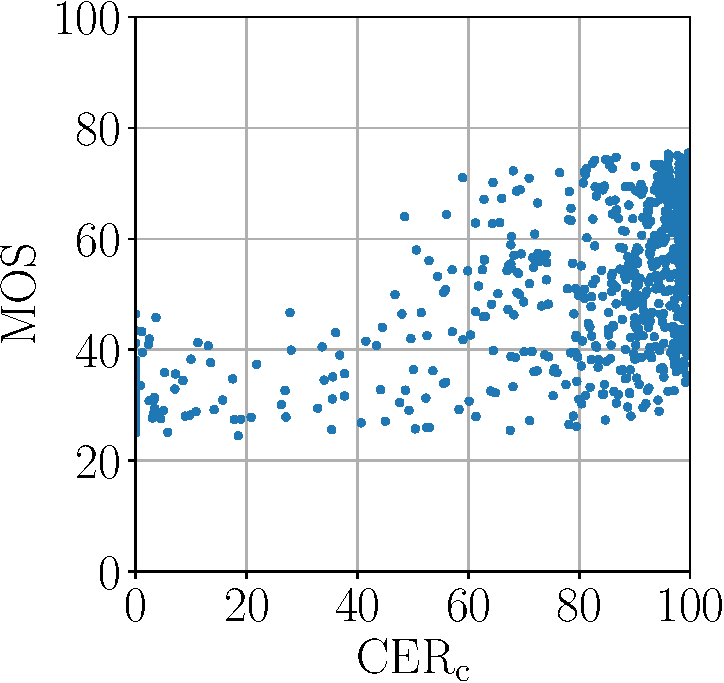
\includegraphics[width=\textwidth]{../../images/cer_mos_overview_ref_tess.pdf}
        \caption{CER vs MOS for Tesseract \gls{ocr} and the pseudo \gls{gt}.}
        \label{fig:cer_vs_mos_ref_tess}
    \end{subfigure}
    \hfill
    \begin{subfigure}[b]{0.45\textwidth}
        \centering
        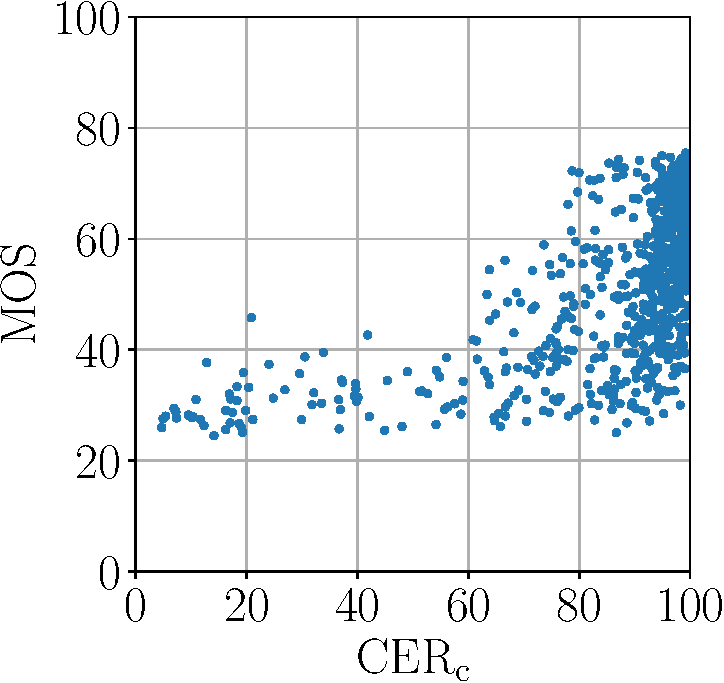
\includegraphics[width=\textwidth]{../../images/cer_mos_overview_ref_ezocr.pdf}
        \caption{CER vs MOS for EasyOCR and the pseudo \gls{gt}.}
        \label{fig:cer_vs_mos_ref_ocr}
    \end{subfigure}
    \caption{$\text{CER}_{\text{c}}$ vs \gls{mos} for Tesseract \gls{ocr} and EasyOCR, with the true \gls{gt} and the pseudo \gls{gt}.}
    \label{fig:cer_vs_mos_overview}
\end{figure}

In \autoref{fig:cer_vs_mos_overview} the $\text{CER}_{\text{c}}$ is plotted against the \gls{mos} for both \gls{ocr} algorithms and both \glspl{gt}.
Generally, we observe that the \gls{mos} ranges from 20 to 80 for all figures.
On the other hand, the $\text{CER}_{\text{c}}$ spans from 0 to 100 for all figures.
Comparing Tesseract \gls{ocr} with EasyOCR for the true \gls{gt}, we observe that the $\text{CER}_{\text{c}}$ distribution for Tesseract \gls{ocr} is more spread out with more lower $\text{CER}_{\text{c}}$ values compared to EasyOCR
Additionally, there are some points with zero $\text{CER}_{\text{c}}$ for Tesseract \gls{ocr}.
This implies that EasyOCR performs better in general and that Tesseract \gls{ocr} struggles with some distortions and fails to predict anything.
We notice similar behavior when comparing the pseudo \glspl{gt} for both \gls{ocr} algorithms, although the $\text{CER}_{\text{c}}$ values are generally higher.
This can be attributed to the fact that the predictions contain no additional errors due to positioning of the text elements and are generally closer to the pseudo \gls{gt} compared to the true \gls{gt}.
Lastly, it is worth noting that there are minimal occurrences of high \gls{mos} values paired with low $\text{CER}_{\text{c}}$ values, which is evident in the top left sections of all figures.
In the following section we detail the extension of the dataset with compressed images that are used to compare two video codecs.


\section{Extension of the Dataset with Images Distorted by Compression Methods}
\label{sec:dataset_codec}

In this section, we first introduce the two video codecs, the \gls{hevc} and the \gls{vvc}.
We further, explain how the two codecs are adjusted for \glspl{sci} by using screen content extensions.
Finally, we use these codecs for the extension of the dataset by encoding the reference images.

\subsection{High Efficiency Video Coding}
\label{subsec:hevc}

The \gls{hevc} \cite{hevc_2012} is one of the newest video codecs.
It is the successor of the H.264/MPEG-4 AVC codec.
The main improvements were the leveraging of parallel processing architecture in modern devices and addressing higher resolutions.
The codec uses the conventional approach of dividing the image into block shaped regions.
The information about the block size is added to the bit stream sent to the decoder.
The first image of a video sequence uses intraframe prediction, which uses information from neighboring blocks to predict the information in the current block.
For further frames, interframe prediction is used, which leverages the difference from the previous frame to encode the current frame.
This improves coding efficiency, since the difference between frames is usually cheaper to encode than a whole new frame.
However, in our case we only encode single images, so the codecs only use the intraframe prediction.
After predicting the current block, the residual, which represents the difference between the prediction and the original block, is transformed by a linear spatial transform to generate the transform coefficients.
Those are scaled, quantized and entropy coded to further reduce the bit rate.
The prediction information, the transform coefficients and all other required information is then sent to the decoder.
The decoder uses that information to predict the current block as well by replicating the encoder.
Afterwards, the transform coefficients can be reconstructed and used to approximate the residual of the block.
The residual is then added to the prediction to reconstruct the original block.
Further, it employs a number of new techniques over its predecessors to provide around 50\% bit rate savings for equivalent quality.
To conform to the special characteristics of \glspl{sci}, a screen content extension was developed for the \gls{hevc} \cite{hevc_scc_2015}.
We will expand on this in the following subsection after we introduce the \gls{vvc}, as they share some similarities.
For this thesis, we use version 16.21+SCM-8.8 of the HM reference software \cite{hevc_software_2020} to encode the images with the \gls{hevc} codec.
The default \cite{config_hevc_2013} and \gls{scc} \cite{config_hevc_scc_2015} configurations used for encoding are applied according to the common test conditions for color space RGB 444.

\subsection{Versatile Video Coding}
\label{subsec:vvc}

The \gls{vvc} \cite{vvc_2021} is the successor of the \gls{hevc} and one of the most recent video codecs.
Compared to the \gls{hevc}, it introduces combined inter-/intraframe prediction, luma mapping with chroma scaling and additional loop filters.
Additionally, while most implementations of the \gls{hevc} are only able to use square block sizes, the \gls{vvc} supports rectangular block sizes as well, which enables more efficient coverage of regions that can be encoded efficiently.
It aims to reach another 50\% bit rate savings compared to the \gls{hevc} for equivalent quality.
Further, the versatility of the codec enables it to be used for a wider range of applications, including $360^{\circ}$ immersive video, high dynamic range, adaptive streaming with resolution changes and many more.
For this thesis, we use version 17.2 of the VTM reference software \cite{vvc_software_2022} to encode the images with the \gls{vvc} codec.
The default and \gls{scc} \cite{config_vvc_both_2020} configurations used for encoding are applied according to the common test conditions for color space RGB 444.

For \glspl{sci} there are some additional tools \cite{vvc_2021} to improve the performance of the codecs due to the different characteristics of the images.
One such tool is the palette mode, which uses a reduced number of colors to encode blocks of images, because \glspl{sci} generally contain a limited amount of colors in local regions.
This tool exists for the \gls{hevc}, but is further improved in the \gls{vvc}.
Another tool is the intra-picture block copy, which enables the codecs to use a copy of a block as the prediction for another block,
It leverages the fact that \glspl{sci} often contain repeated patterns, for instance in the form of UI elements or large uniformly colored regions.
In the \gls{hevc} screen content extension, this tool is able to copy blocks from the same frame from further away, while in the \gls{vvc} the complexity is reduced by restricting the copying to neighboring blocks.
\begin{figure}
    \centering
    \begin{subfigure}[b]{0.45\textwidth}
        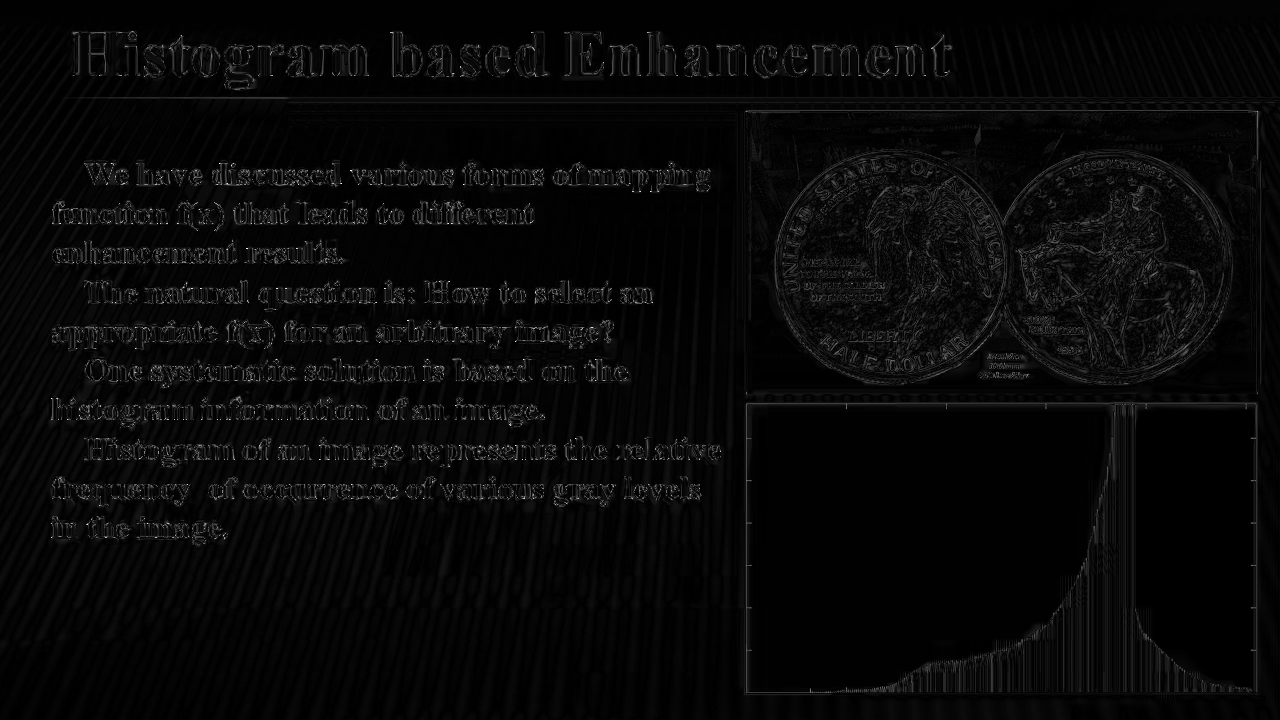
\includegraphics[width=\linewidth]{../images/codec_hm_default_diff_50_SCI4.png}
        \caption{Default configuration}
        \label{fig:codec_hm_default_diff_50_SCI4}
    \end{subfigure}
    \hfill
    \begin{subfigure}[b]{0.45\textwidth}
        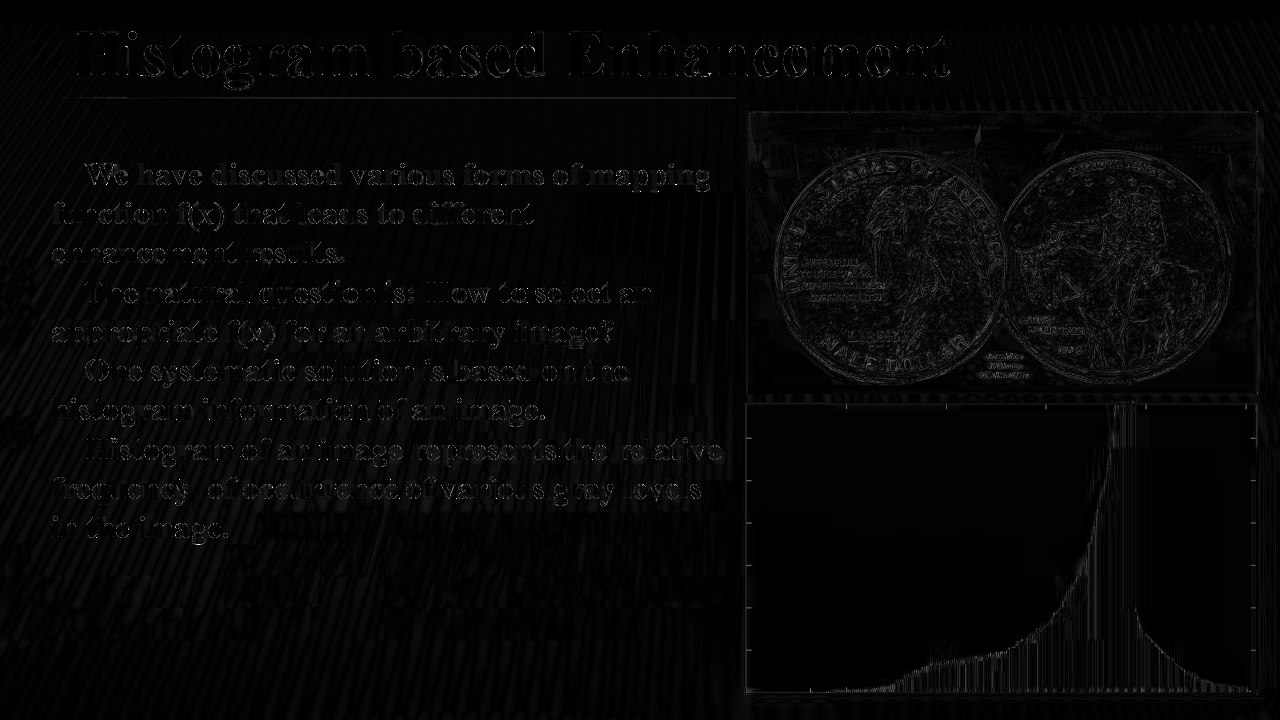
\includegraphics[width=\linewidth]{../images/codec_hm_scc_diff_50_SCI4.png}
        \caption{\gls{scc} configuration}
        \label{fig:codec_hm_scc_diff_50_SCI4}
    \end{subfigure}
    \caption{Normalized absolute pixel differences between the reference image and the \gls{hevc} encoded images with the default and \gls{scc} configurations for Image 4.}
    \label{fig:codec_hm_diff_50_SCI4}
\end{figure}
The improvements from the screen content tools for \gls{hevc} are evident when observing \autoref{fig:codec_hm_diff_50_SCI4}.
The figures depict the normalized absolute pixel differences between a reference image and its corresponding encoded image, with brighter pixels representing a larger difference.
Notably, the absolute pixel differences, representing the coding error, are reduced for the \gls{scc} configuration compared to the default configuration, particularly in the text regions.
\begin{figure}
    \centering
    \begin{subfigure}[b]{0.45\textwidth}
        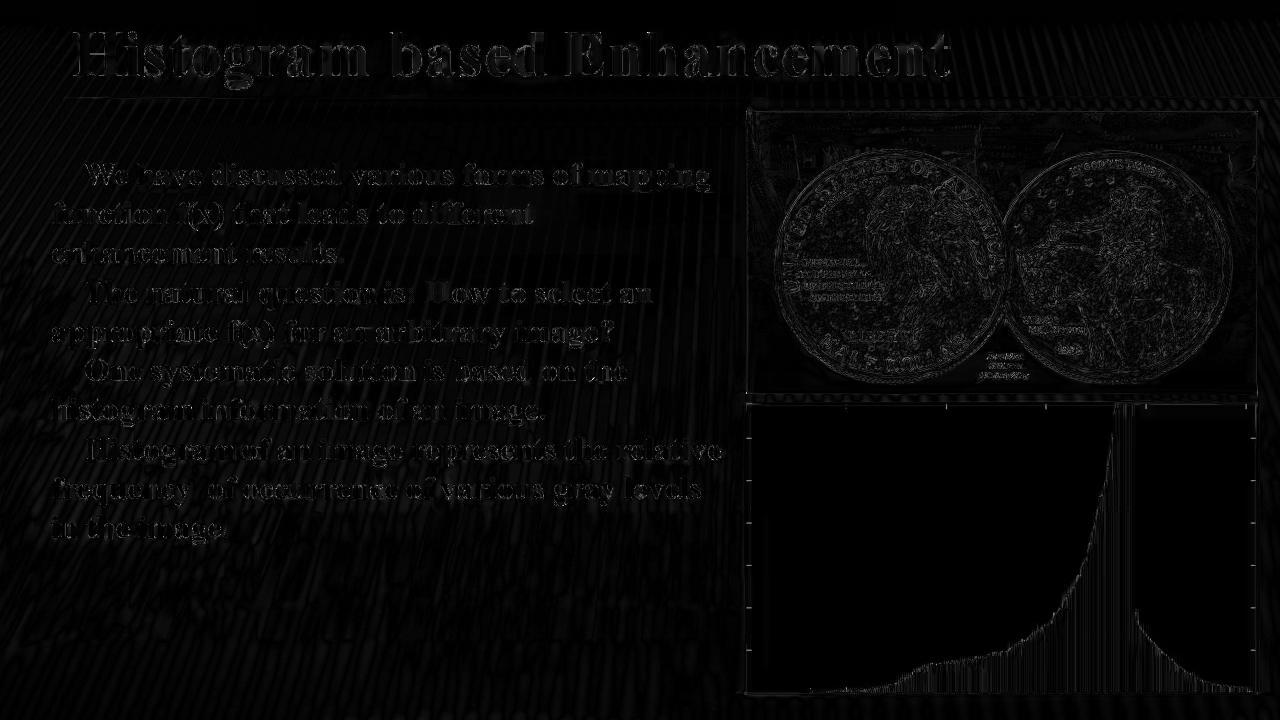
\includegraphics[width=\linewidth]{../images/codec_vtm_default_diff_50_SCI4.png}
        \caption{Default configuration}
        \label{fig:codec_vtm_default_diff_50_SCI4}
    \end{subfigure}
    \hfill
    \begin{subfigure}[b]{0.45\textwidth}
        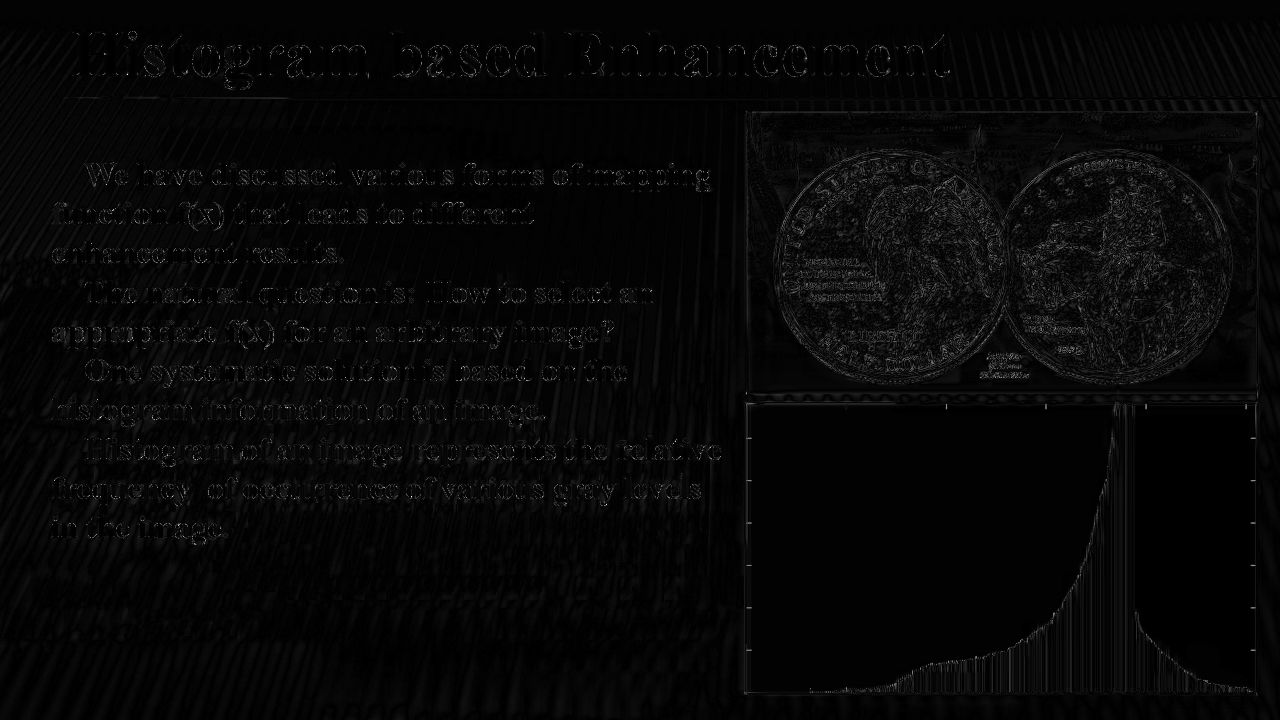
\includegraphics[width=\linewidth]{../images/codec_vtm_scc_diff_50_SCI4.png}
        \caption{\gls{scc} configuration}
        \label{fig:codec_vtm_scc_diff_50_SCI4}
    \end{subfigure}
    \caption{Normalized absolute pixel differences between the reference image and the \gls{vvc} encoded images with the default and \gls{scc} configurations for Image 4.}
    \label{fig:codec_vtm_diff_50_SCI4}
\end{figure}
A similar, albeit more subtle difference is observable for \gls{vvc} in \autoref{fig:codec_vtm_diff_50_SCI4}.


It is to note, that we use these codecs on images instead of videos, which implies that we are not leveraging the full potential of the videos codecs.
To extend the dataset we encode the reference images with the default and the \gls{scc} configuration of the codecs.
The most important difference to the other distorted images is that there are no subjective scores available for these images.
However, we can use more images for the comparison of the codecs, as we do not need to select based on too much focus on graphical objects over the text elements.
For the experiments related to the codecs we select the images with
\begin{equation}
    i \in \{1, 2, 3, 4, 5, 6, 7, 8, 9, 11, 12, 13, 15, 16, 18, 19, 20, 21, 22, 23, 24, 25, 27, 29\}.
\end{equation}
The common test condition \glspl{qp} $\in \{22, 27, 32, 37\}$ result in no significant changes in the $\text{CER}_{\text{c}}$.
Therefore, following the approach of previous researchers in \cite{ultra_low_bitrate_2022}, we encode these images with \glspl{qp} $\in \{35, 40, 45, 50\}$ for both codecs.
We subsequently employ the \gls{ocr} algorithms to extract text from these images, enabling us to compute the $\text{CER}_{\text{c}}$.
Afterwards, we can visualize rate-distortion curves and calculate the \gls{bdrate}, as described in \autoref{subsec:bdrate}.

In summary, the original dataset contains a \gls{mos} for each image with various distortions.
To evaluate the performance of the \gls{ocr} algorithms, we create text labels for each of the images.
Further, we expand the dataset by encoding select reference images with the \gls{hevc} and \gls{vvc} codecs.
With all the necessary components to describe the experiments now in place, we proceed to evaluate and discuss our results in the subsequent chapter.

    \chapter{Evaluation}
\label{chap:evaluation}

In this chapter, we first go over the performance of the \gls{ocr} algorithms.
Then we compare the performance of the \gls{ocr} algorithms against human judgment.
Additionally, we investigate the feasibility of using recognized text from pristine images as ground truth.
Finally, we evaluate the performance of the \gls{ocr} algorithms on different quality levels of the HM and VTM codecs.

\section{Performance of Optical Character Recognition}
\label{sec:ocr_performance}

First, we evaluate the impact of different distortion types on \gls{ocr} performance by comparing the mean \gls{cer} for various quality levels.
This analysis is performed separately for EasyOCR and Tesseract \gls{ocr} to determine which performs better.

For the comparison, we plot the mean \gls{cer} with regards to the \gls{gt} on the y-axis against different quality levels on the x-axis.
We do this for all the distortion types.

\begin{figure}[h]
\centering
    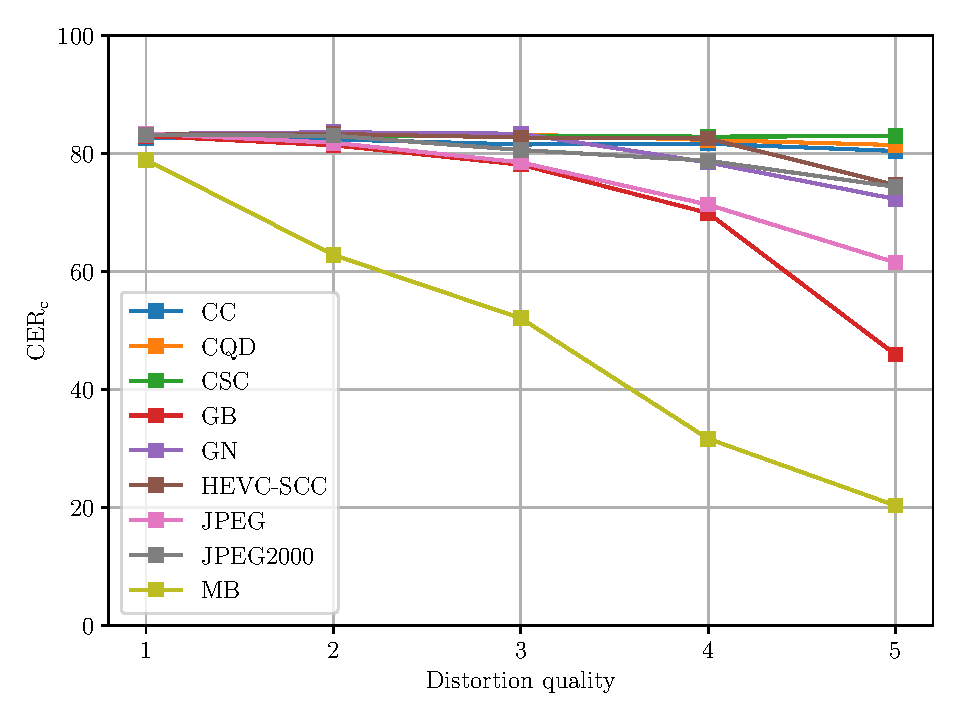
\includegraphics[width=\textwidth]{../../images/analyze/cer_dist_quality_gt_ezocr.pdf}
    \caption{Mean \gls{cer} in relation to the \gls{gt} for different quality levels with EasyOCR.}
\label{fig:cer_dist_quality_gt_ezocr}
\end{figure}

In \autoref{fig:cer_dist_quality_gt_ezocr}, we observe the mean \gls{cer} in relation to the ground truth (\gls{gt}) for different quality levels using EasyOCR.
A noticeable trend is that motion blur has the most significant impact on EasyOCR's performance, exhibiting a nearly linear decrease from 80 to 20.
Both JPEG and Gaussian blur display similar behavior until quality level 4, after which Gaussian blur experiences a steeper decline.
Notably, the blurring of images greatly affects the legibility of text, with letters becoming indistinct and merging together, resulting in the poorest performance for EasyOCR.
Gaussian noise, JPEG2000, and HEVC-SCC exhibit comparable performance, all experiencing a decline at quality level 5.
The remaining distortions have minimal impact on performance, which is expected since color distortions do not directly affect text shapes.

\begin{figure}[h]
\centering
    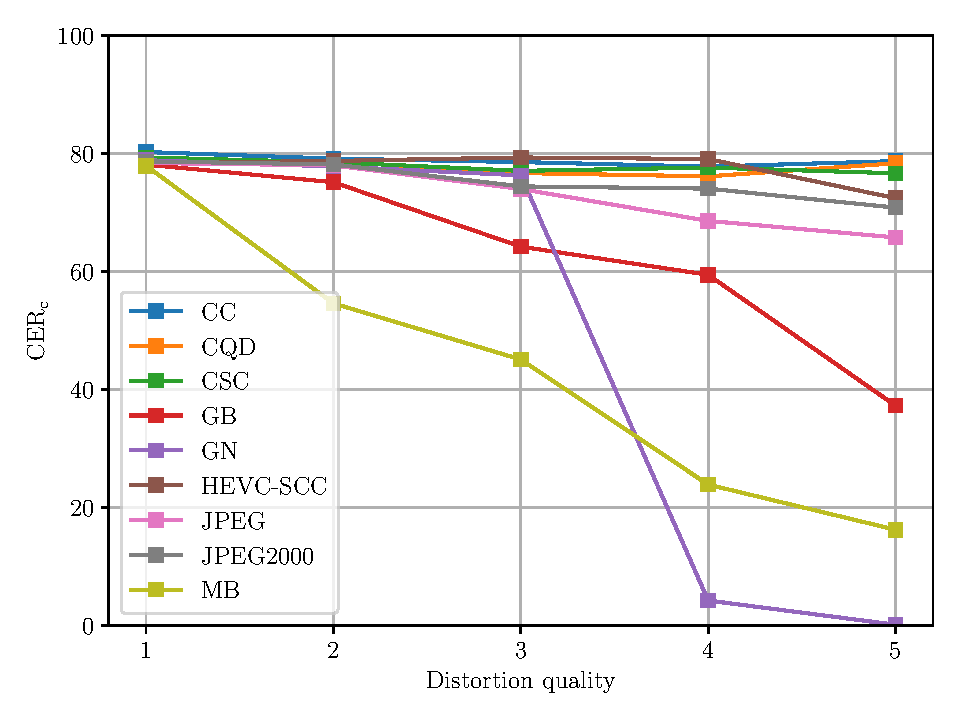
\includegraphics[width=\textwidth]{../../images/analyze/cer_dist_quality_gt_tess.pdf}
    \caption{Mean \gls{cer} in relation to the \gls{gt} for different quality levels with Tesseract \gls{ocr}.}
\label{fig:cer_dist_quality_gt_tesseract}
\end{figure}

In \autoref{fig:cer_dist_quality_gt_tesseract}, we observe the mean \gls{cer} plotted in relation the ground truth (\gls{gt}) for various quality levels using Tesseract \gls{ocr}.
A steady decrease in \gls{cer} can be seen for motion blur and Gaussian blur, with the former exhibiting a 20-point higher value compared to the latter.
However, the most noteworthy finding is the significant drop in \gls{cer} for Gaussian noise at quality level 4, reaching 0 at quality level 5.
This sudden decline is particularly surprising when compared to other types of distortions.
Among the distortions analyzed, CC, CQD, and CSC perform the best, with CC even demonstrating a slightly higher \gls{cer} at quality level 5 compared to previous levels.
This phenomenon can possibly be attributed to CC's ability to enhance the distinction between the text and the background, acting almost like an image preprocessing step for the \gls{ocr}.
Interestingly, the \gls{cer} for HEVC-SCC slightly increases at quality level 4 and then decreases again at quality level 5.
A plausible explanation for this behavior is that certain portions of the text are not well recognized at quality 4, and since these unrecognized parts are not included in the \gls{gt}, it leads to a higher \gls{cer}.
Then at level 5, more parts, that are in the ground truth, are not recognized well.
Consequently, the \gls{cer} decreases.

In summary, our observations reveal that motion blur and Gaussian blur have a substantial impact on the performance of both EasyOCR and Tesseract \gls{ocr} algorithms.
Additionally, both \gls{ocr} algorithms perform demonstrate superior performance across images with CC, CQD, and CSC.
However, the most remarkable discovery is the significant drop in the \gls{cer} for Gaussian noise at quality level 4, reaching 0 at quality level 5, specifically for Tesseract OCR.
This suggests that EasyOCR exhibits greater robustness to Gaussian noise compared to Tesseract \gls{ocr} .
Overall, EasyOCR outperforms Tesseract \gls{ocr} , with a performance ceiling of approximately 83 \gls{cer} for EasyOCR, while Tesseract \gls{ocr} only achieves around 70 \gls{cer}.

\section{Comparison Against Human Judgment}
\label{sec:comparison_against_human_judgment}

In this section, we compare the performance of the \gls{ocr} algorithms with human judgment.
We use the subjective quality scores to investigate the correlation between the \gls{cer} and the \gls{mos}.
However, compared to the last section, we calculate the \gls{cer} in relation to the reference image instead of the ground truth.
This makes it a fairer comparison as the humans that rated the images, compared the distorted images to the reference image to arrive at the \gls{mos}.


% mos vs cer mean in relation to reference for easyocr
\begin{figure}[h]
\centering
    \begin{subfigure}[b]{0.3\textwidth}
        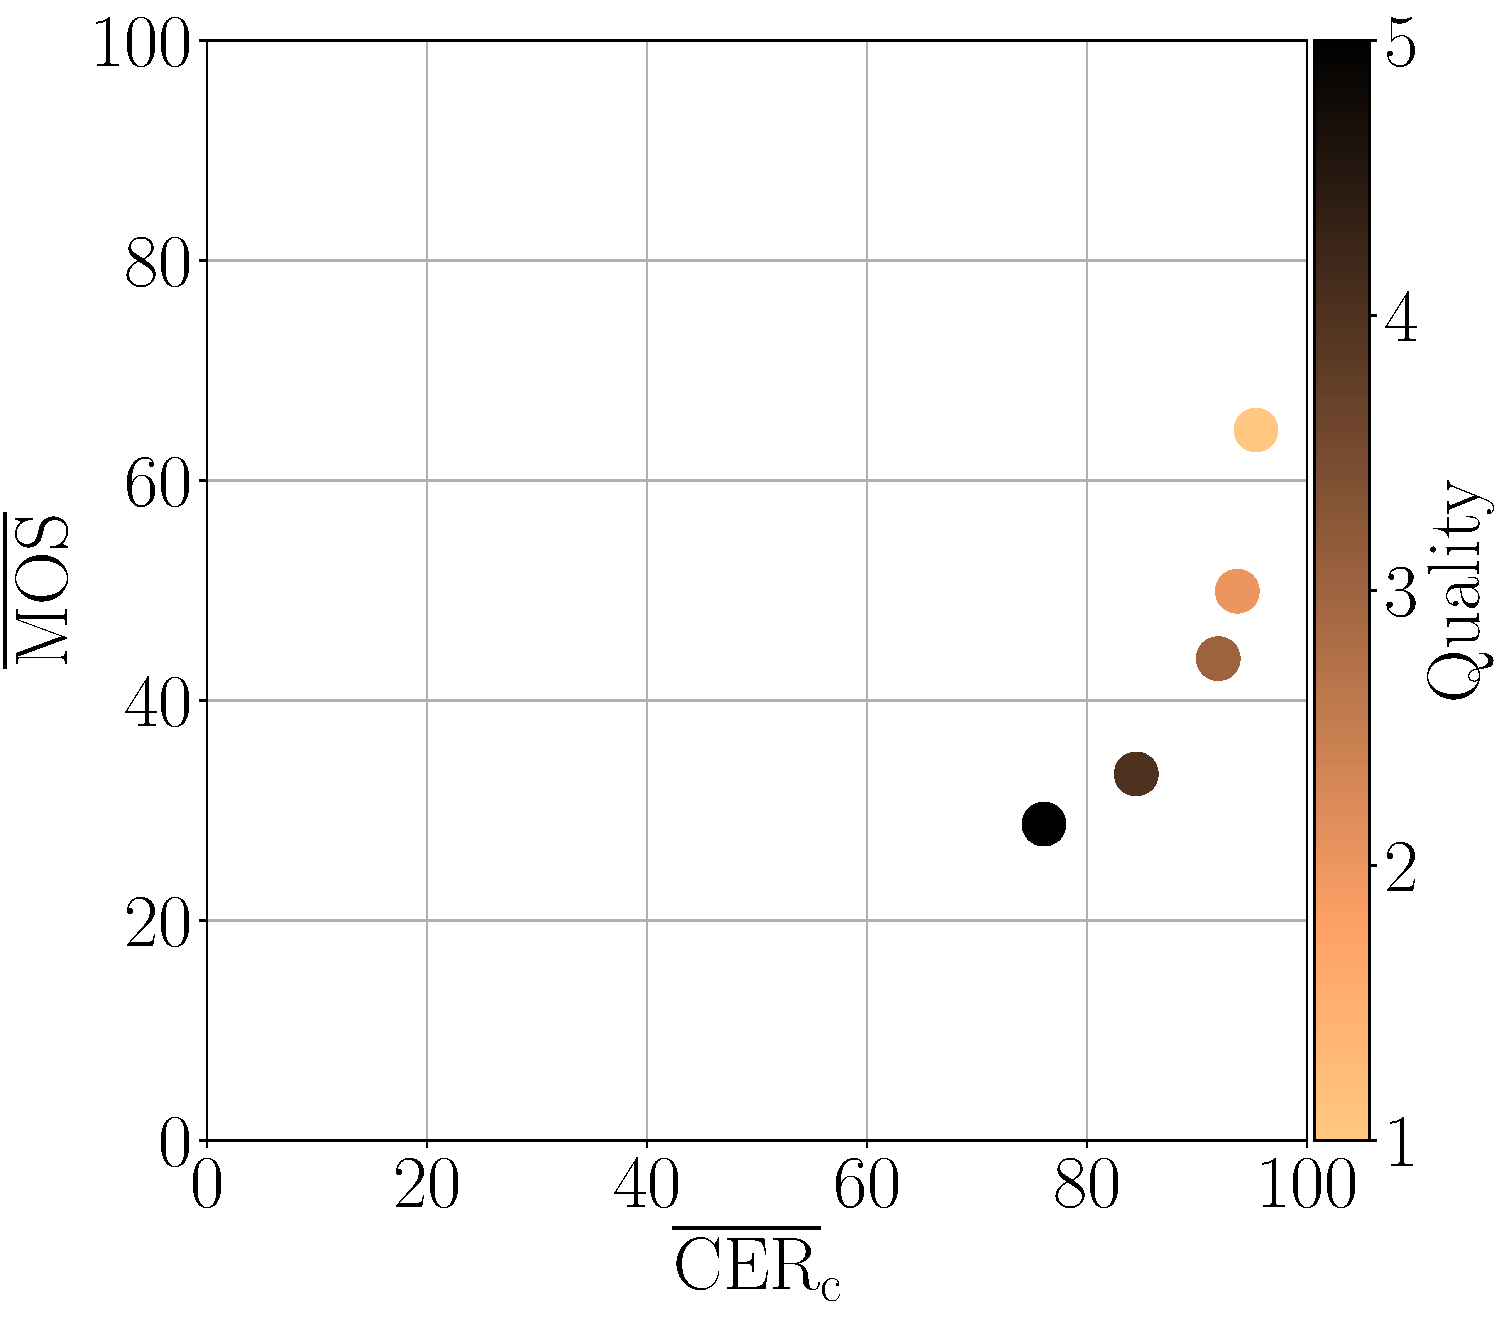
\includegraphics[width=\textwidth]{../../images/analyze/mos_cer_ref_mean_ezocr_GN.pdf}
        \caption{GN}
        \label{fig:mos_cer_ref_mean_ezocr_GN}
    \end{subfigure}
    \hfill
    \begin{subfigure}[b]{0.3\textwidth}
        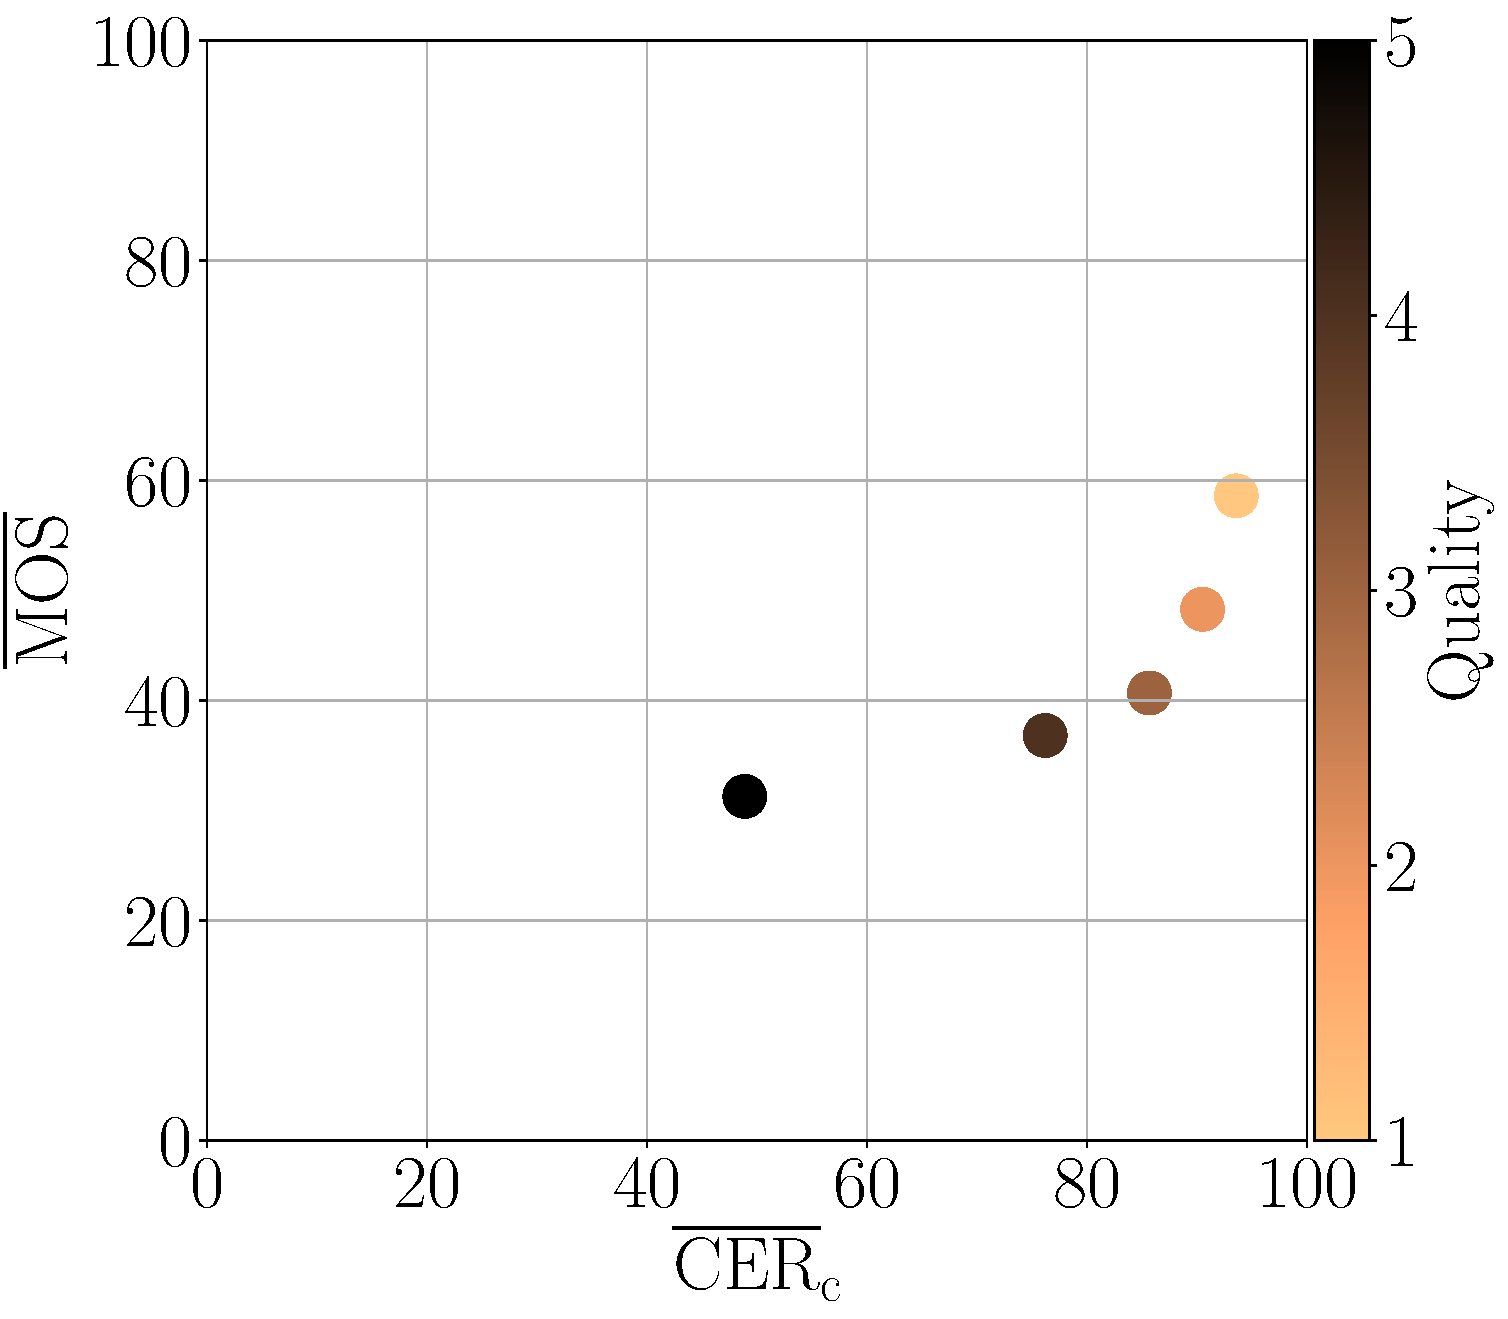
\includegraphics[width=\textwidth]{../../images/analyze/mos_cer_ref_mean_ezocr_GB.pdf}
        \caption{GB}
        \label{fig:mos_cer_ref_mean_ezocr_GB}
    \end{subfigure}
    \hfill
    \begin{subfigure}[b]{0.3\textwidth}
        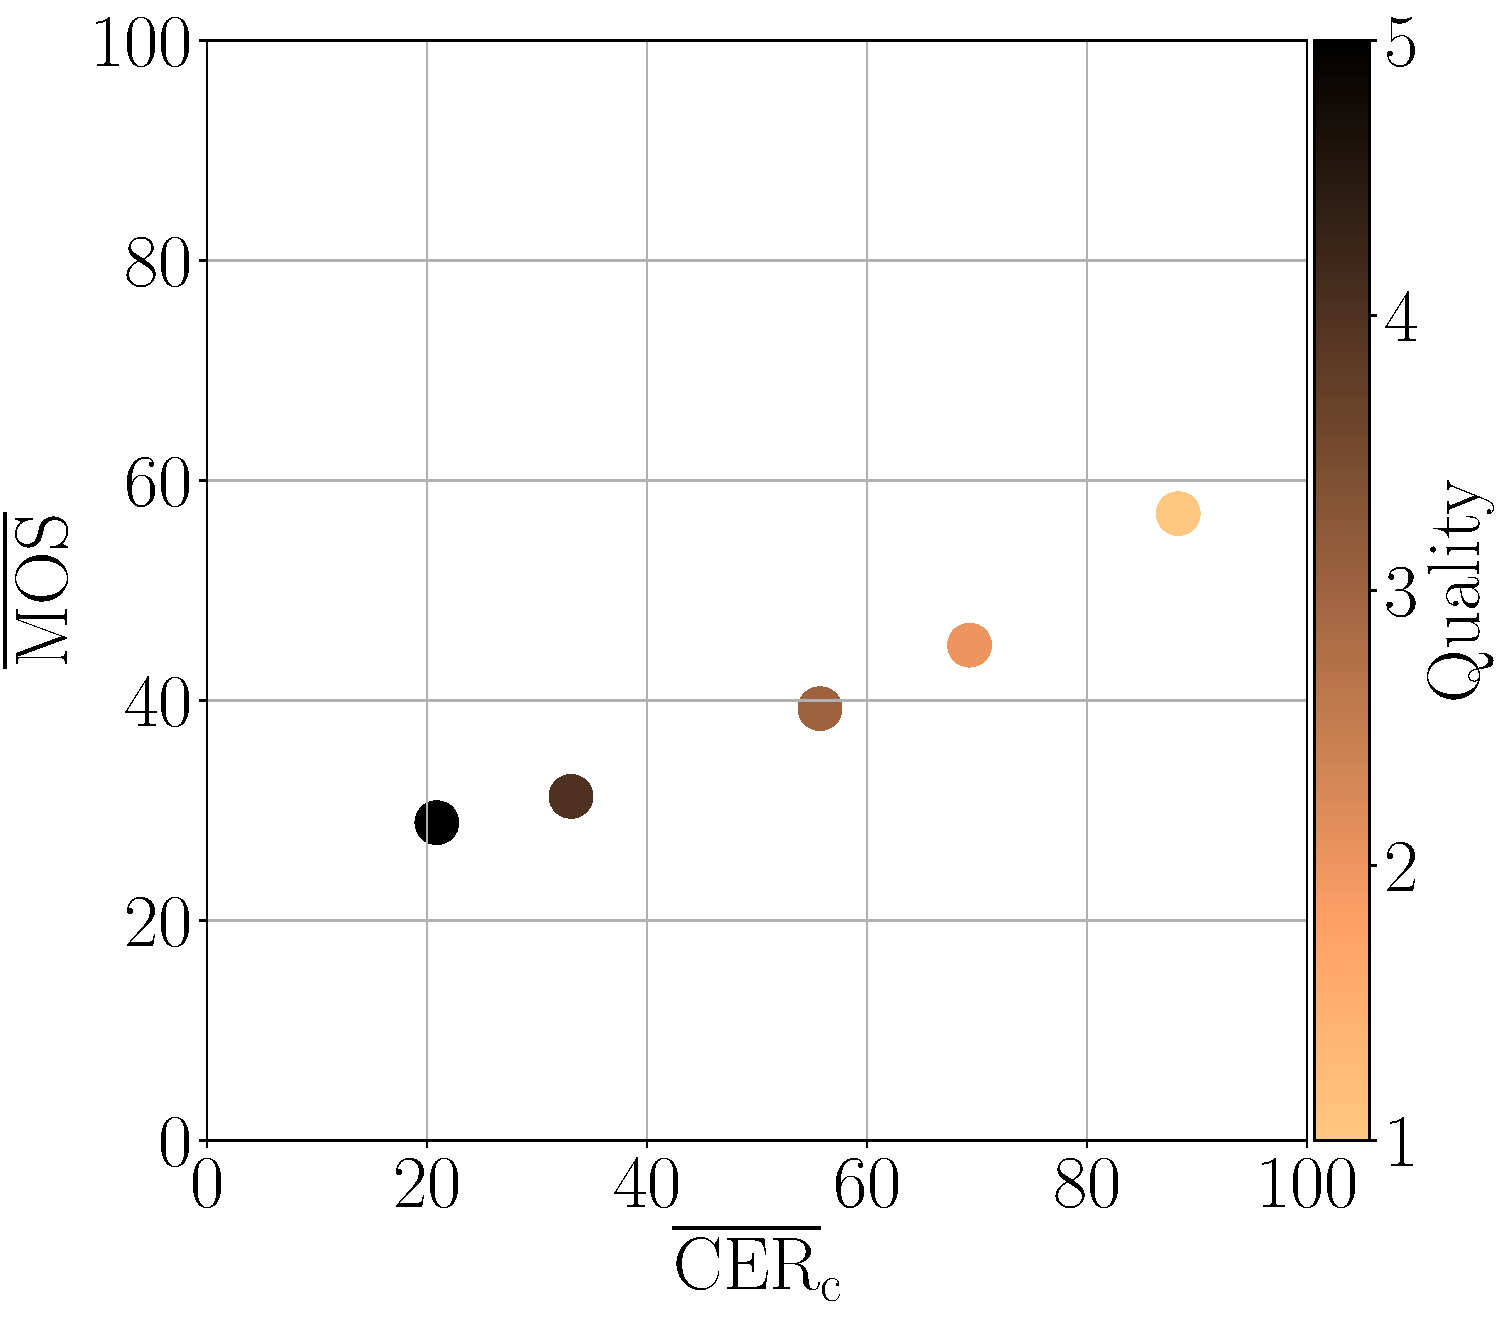
\includegraphics[width=\textwidth]{../../images/analyze/mos_cer_ref_mean_ezocr_MB.pdf}
        \caption{MB}
        \label{fig:mos_cer_ref_mean_ezocr_MB}
    \end{subfigure}
    \newline
    \begin{subfigure}[b]{0.3\textwidth}
        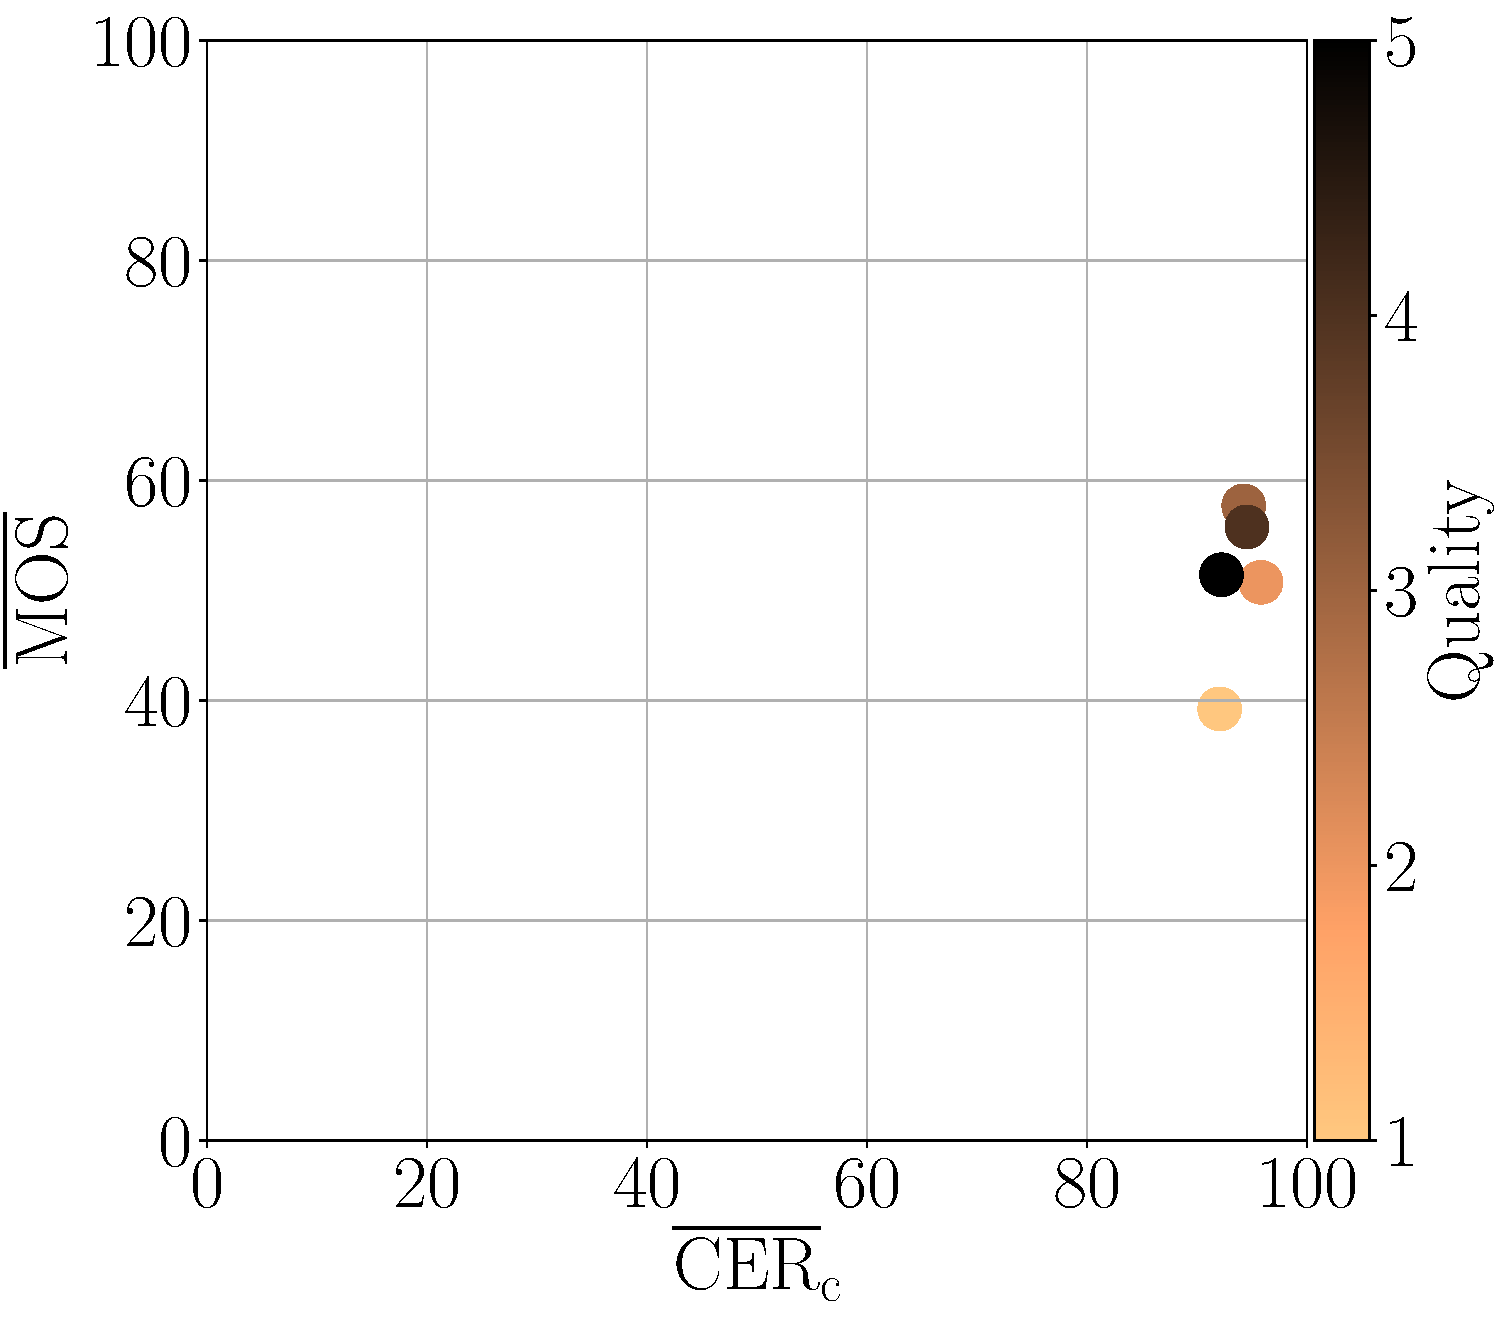
\includegraphics[width=\textwidth]{../../images/analyze/mos_cer_ref_mean_ezocr_CC.pdf}
        \caption{CC}
        \label{fig:mos_cer_ref_mean_ezocr_CC}
    \end{subfigure}
    \hfill
    \begin{subfigure}[b]{0.3\textwidth}
        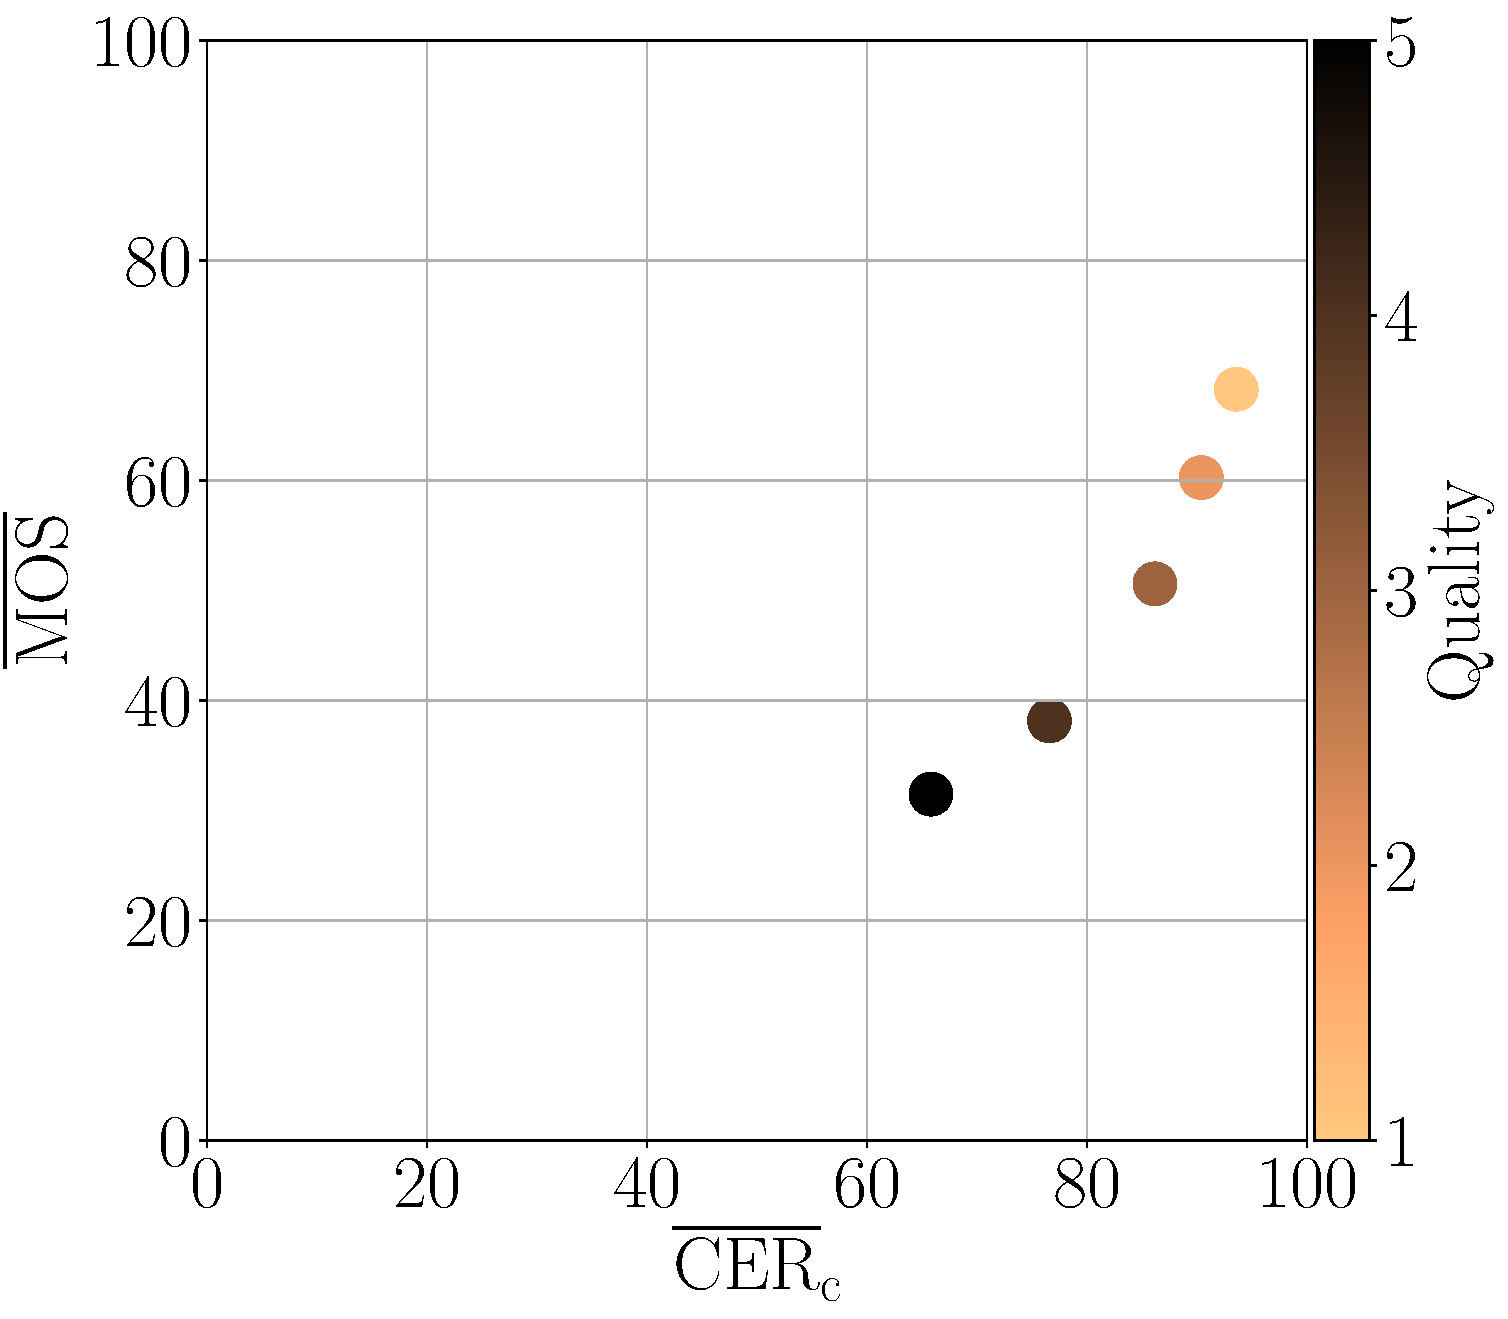
\includegraphics[width=\textwidth]{../../images/analyze/mos_cer_ref_mean_ezocr_JPEG.pdf}
        \caption{JPEG}
        \label{fig:mos_cer_ref_mean_ezocr_JPEG}
    \end{subfigure}
    \hfill
    \begin{subfigure}[b]{0.3\textwidth}
        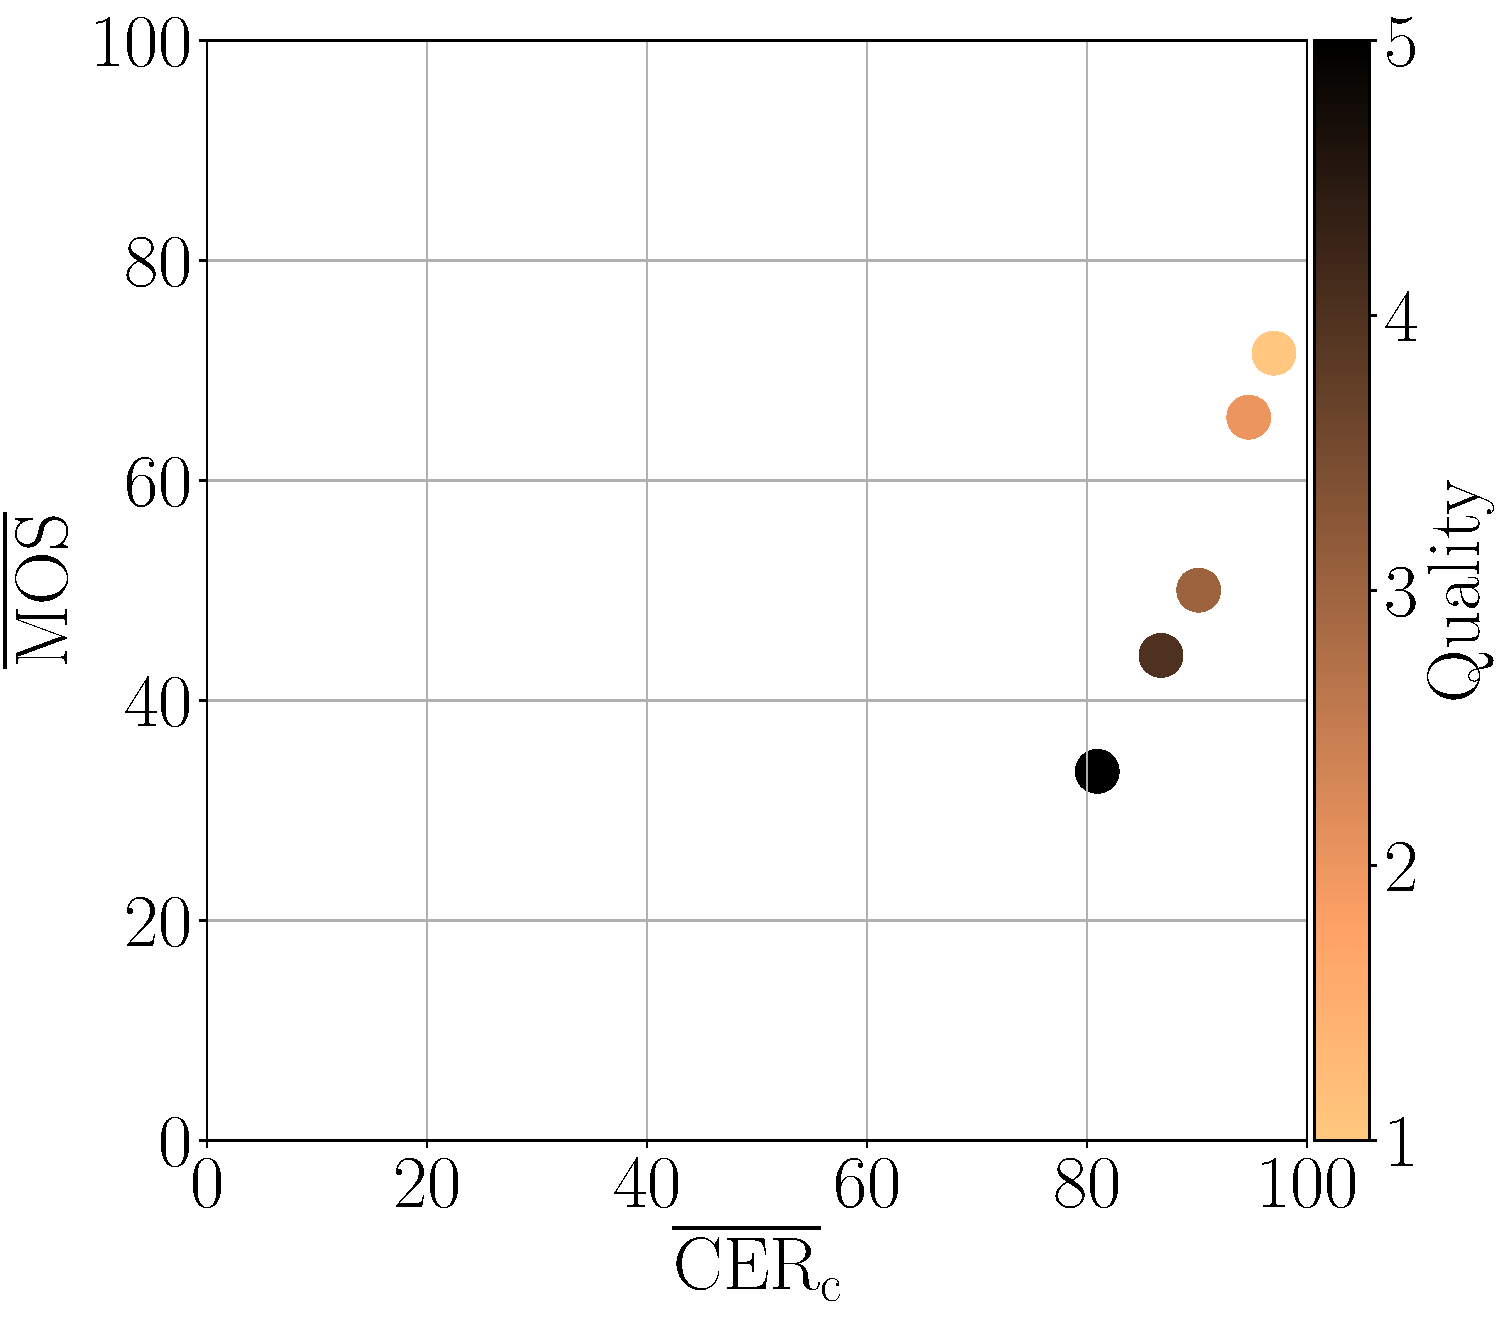
\includegraphics[width=\textwidth]{../../images/analyze/mos_cer_ref_mean_ezocr_JPEG2000.pdf}
        \caption{JPEG2000}
        \label{fig:mos_cer_ref_mean_ezocr_JPEG2000}
    \end{subfigure}
    \newline
    \begin{subfigure}[b]{0.3\textwidth}
        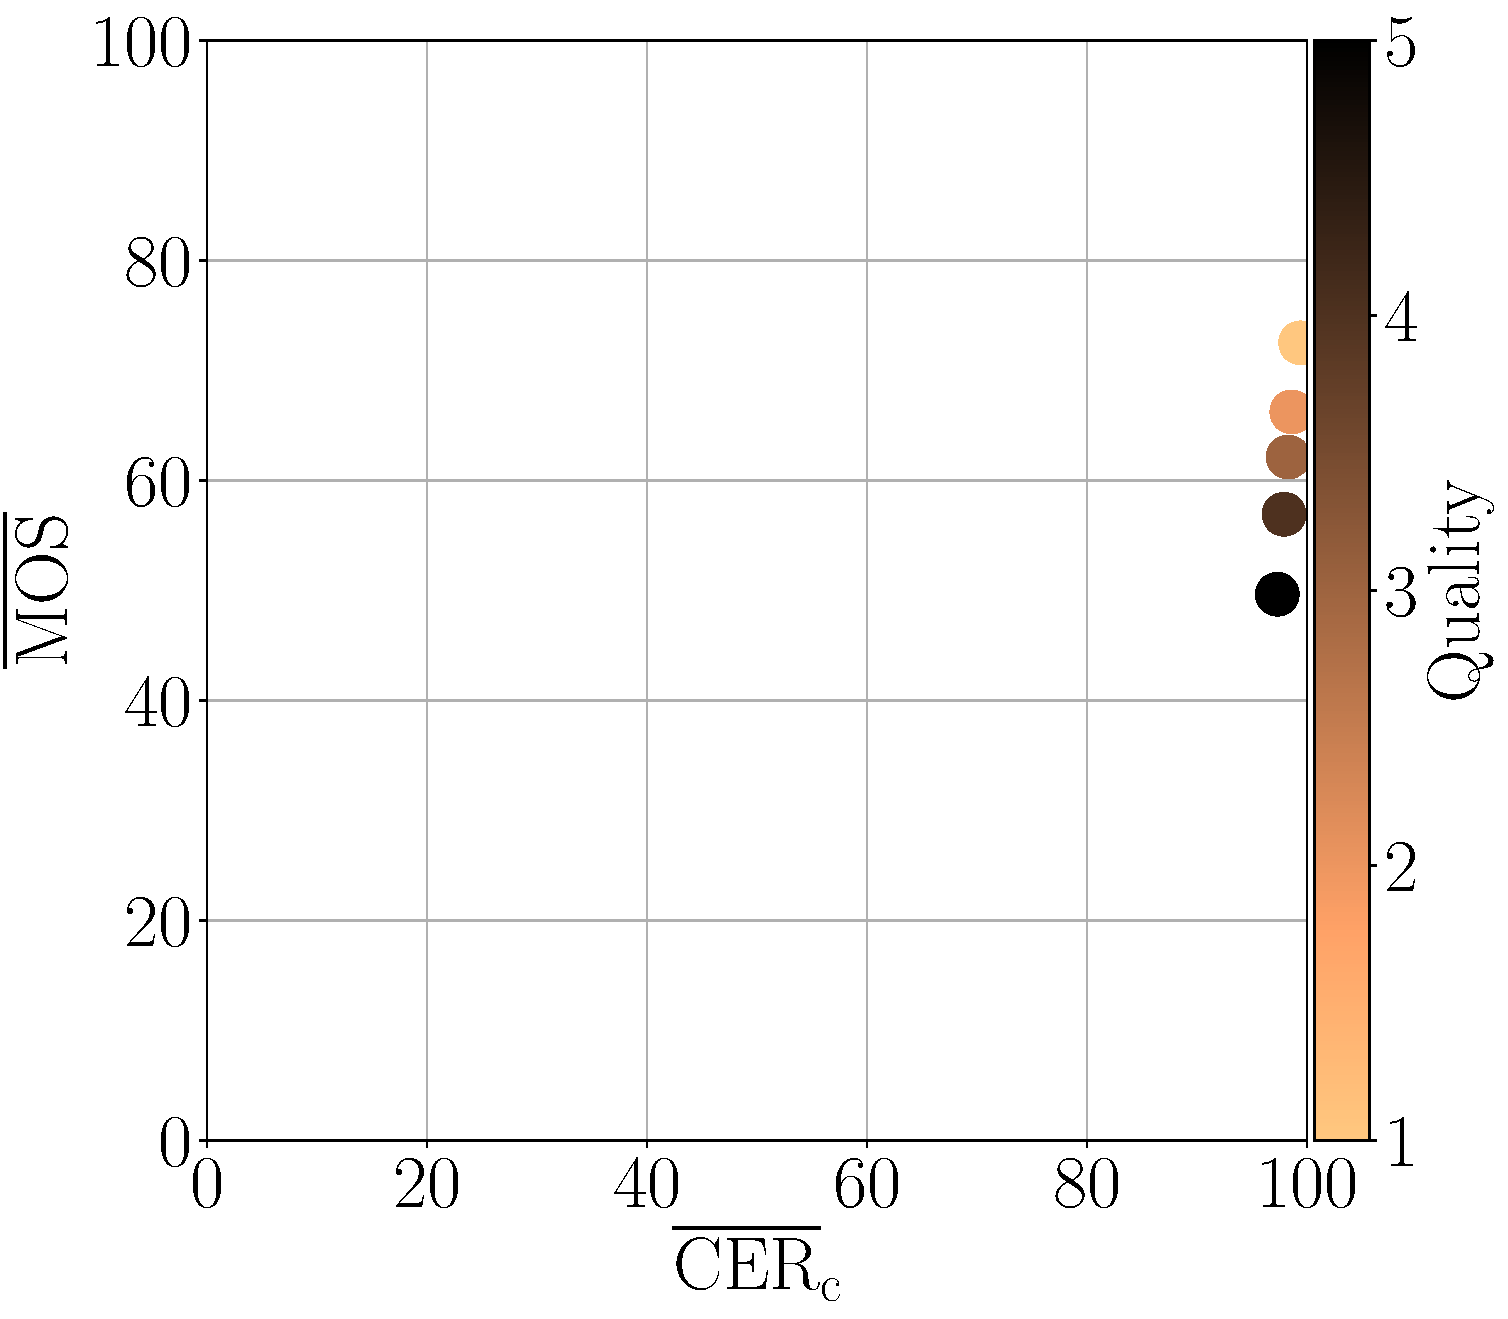
\includegraphics[width=\textwidth]{../../images/analyze/mos_cer_ref_mean_ezocr_CSC.pdf}
        \caption{CSC}
        \label{fig:mos_cer_ref_mean_ezocr_CSC}
    \end{subfigure}
    \hfill
    \begin{subfigure}[b]{0.3\textwidth}
        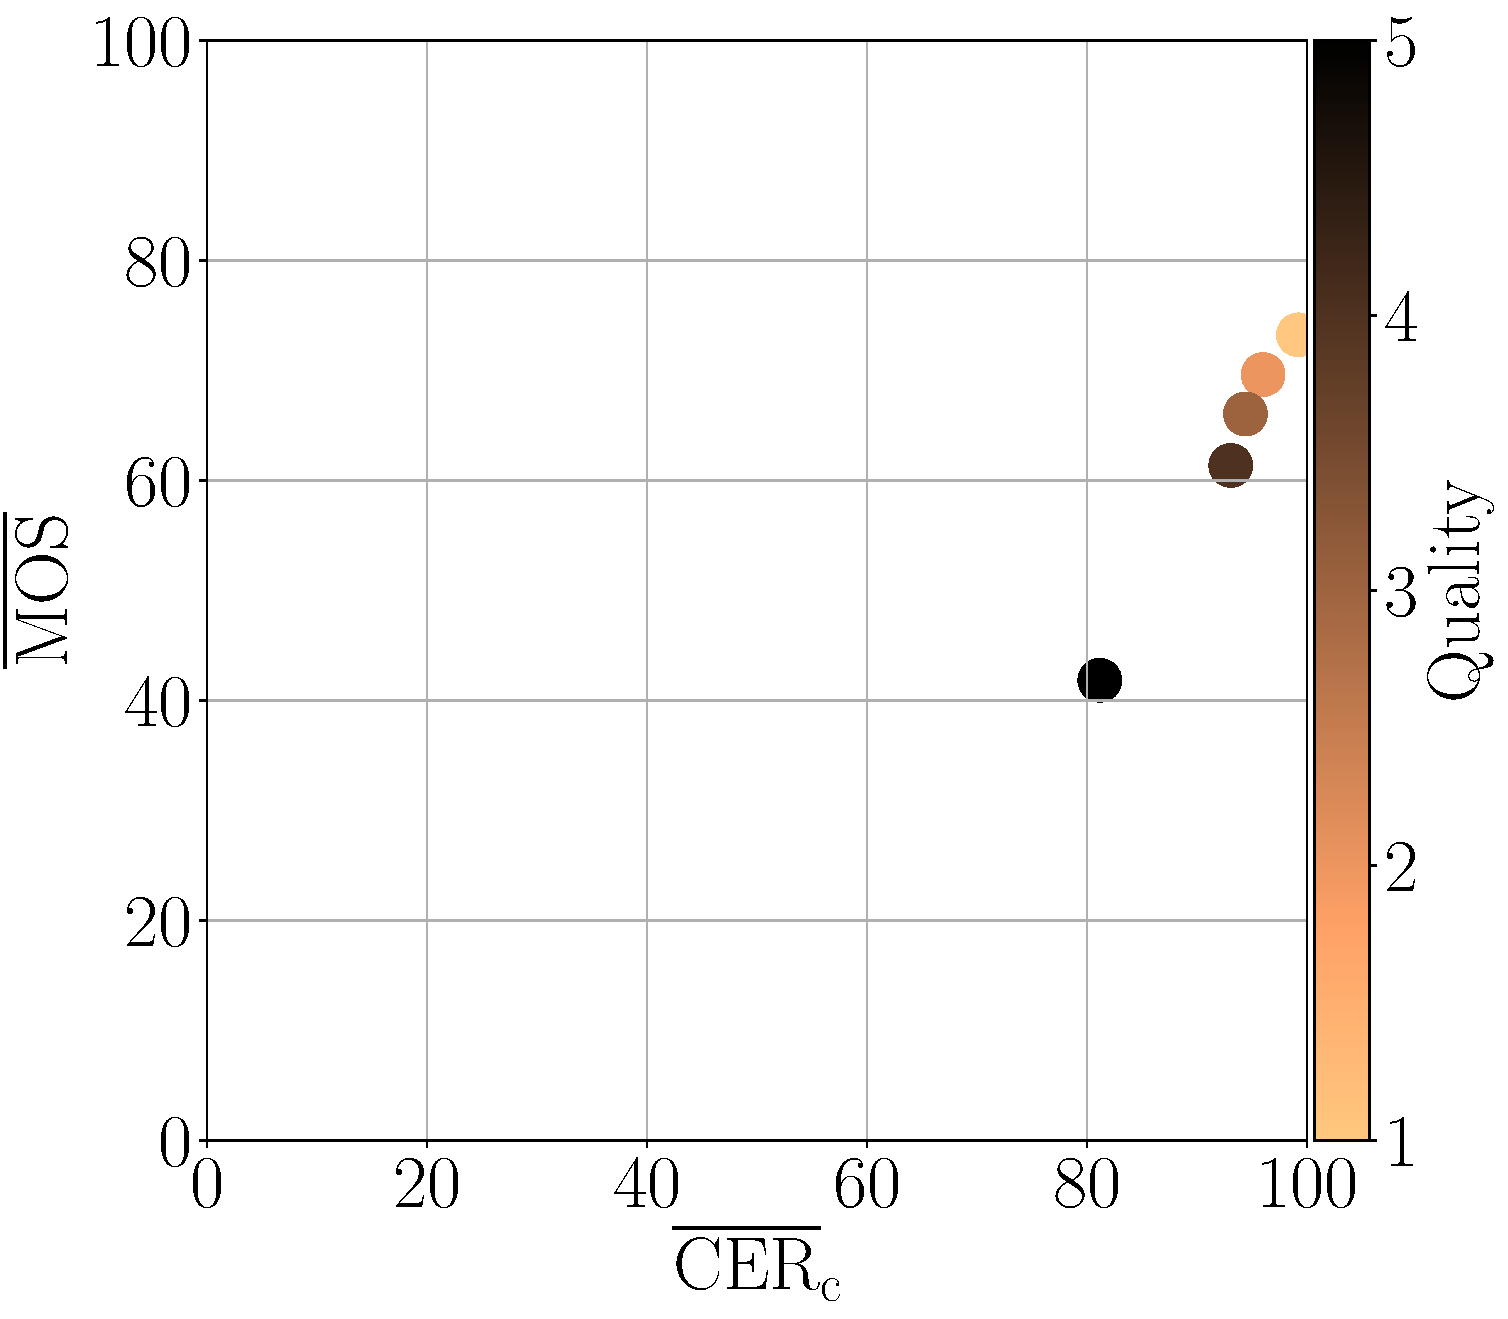
\includegraphics[width=\textwidth]{../../images/analyze/mos_cer_ref_mean_ezocr_HEVC-SCC.pdf}
        \caption{HEVC-SCC}
        \label{fig:mos_cer_ref_mean_ezocr_HEVC-SCC}
    \end{subfigure}
    \hfill
    \begin{subfigure}[b]{0.3\textwidth}
        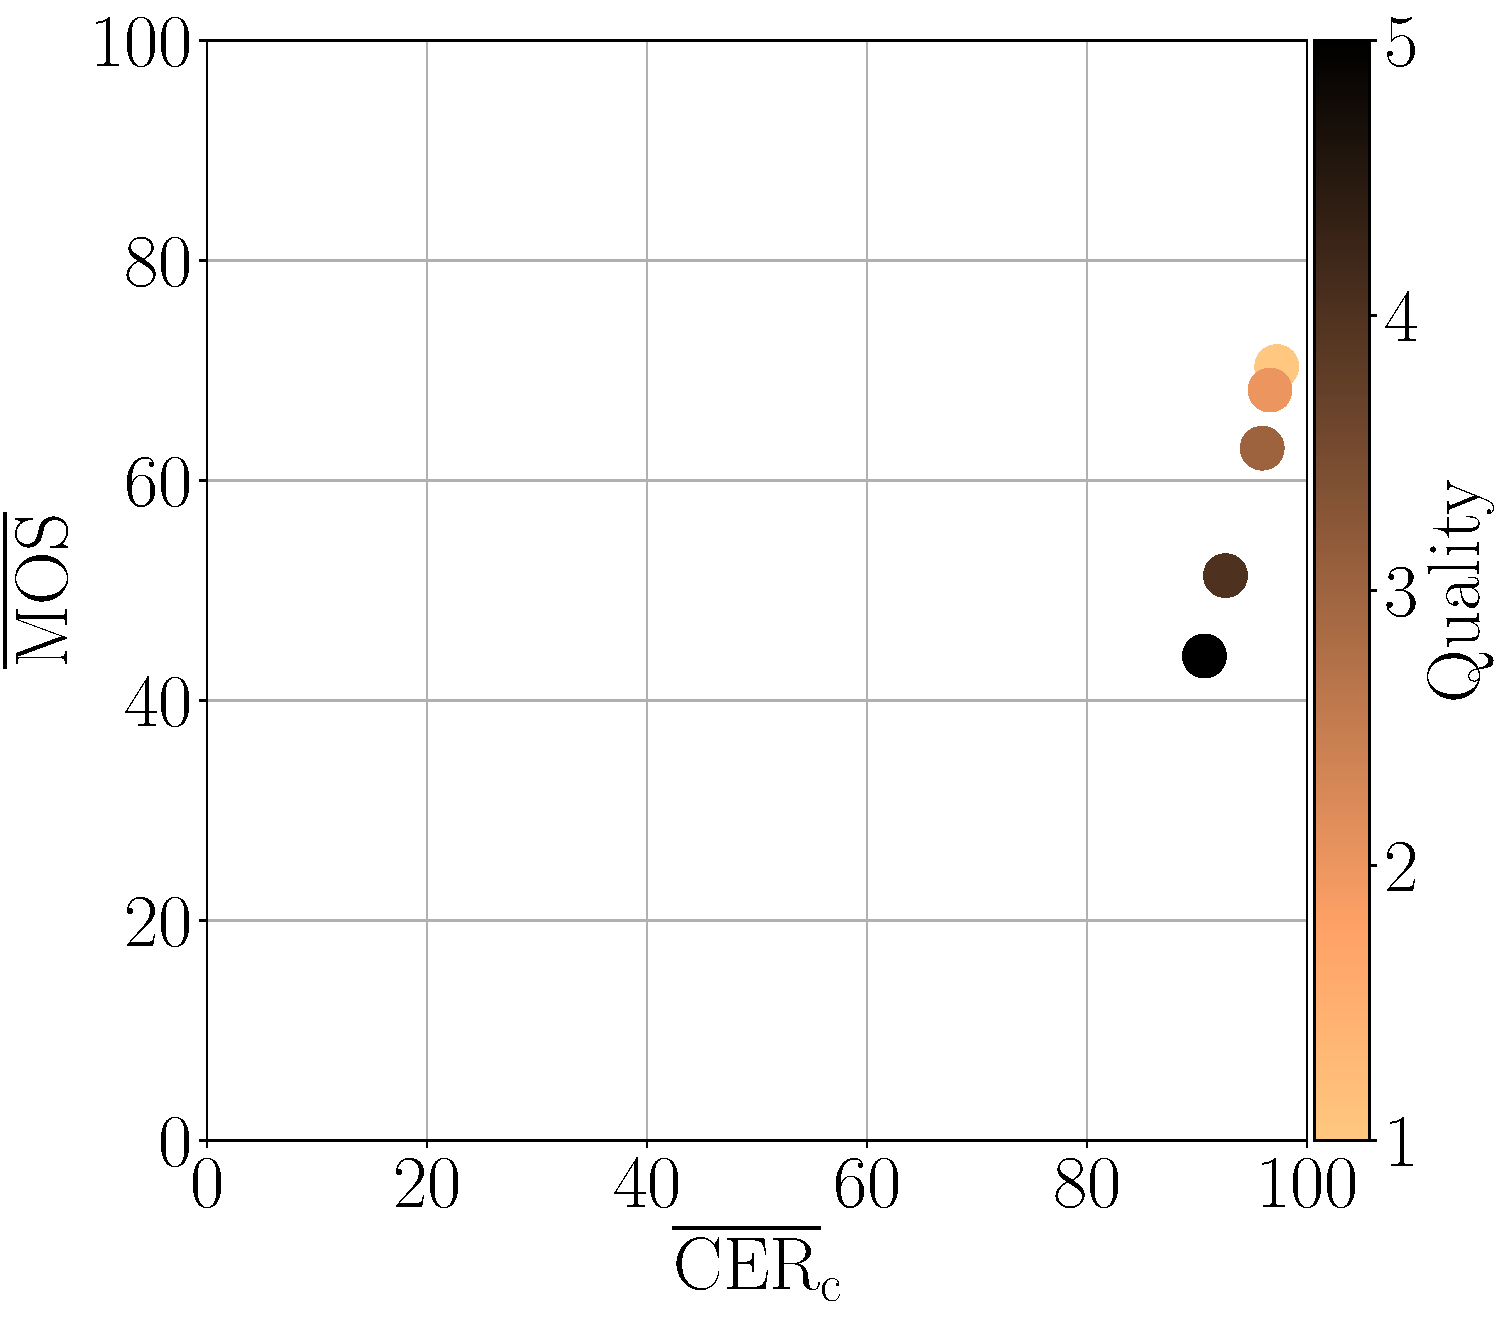
\includegraphics[width=\textwidth]{../../images/analyze/mos_cer_ref_mean_ezocr_CQD.pdf}
        \caption{CQD}
        \label{fig:mos_cer_ref_mean_ezocr_CQD}
    \end{subfigure}
\caption{Mean \gls{cer} in relation to the reference against mean \gls{mos} for different distortion types with EasyOCR.}
\label{fig:mos_cer_ref_mean_ezocr}
\end{figure}

In \autoref{fig:mos_cer_ref_mean_ezocr} we can see the mean \gls{cer} in relation to the reference image against the mean \gls{mos} over selected images for all distortions with EasyOCR.
The first general thing to notice is that the performance ceiling for the \gls{cer} is now up to almost 100.
This is because the \gls{cer} is calculated in relation to the reference image, which is not necessarily the ground truth.
So it is clear, that the performance on CSC and CC are not impacted much by the distortions, as we saw in the previous section.
The \gls{mos} for CSC varies more than the \gls{cer}, but not as much as for other distortion types.
This suggests at least a slight correlation between the \gls{mos} and the \gls{cer}.
For CC neither metric shows a clear trend.
It is not clear why the \gls{mos} for CC is not strictly decreasing with the quality level.
All other distortions show this trend.
Contrast levels do not clearly reach from good to bad, it might be that humans found specific contrast levels more appealing than others.

% mos vs cer mean in relation to reference for Tesseract
\begin{figure}[h]
\centering
    \begin{subfigure}[b]{0.3\textwidth}
        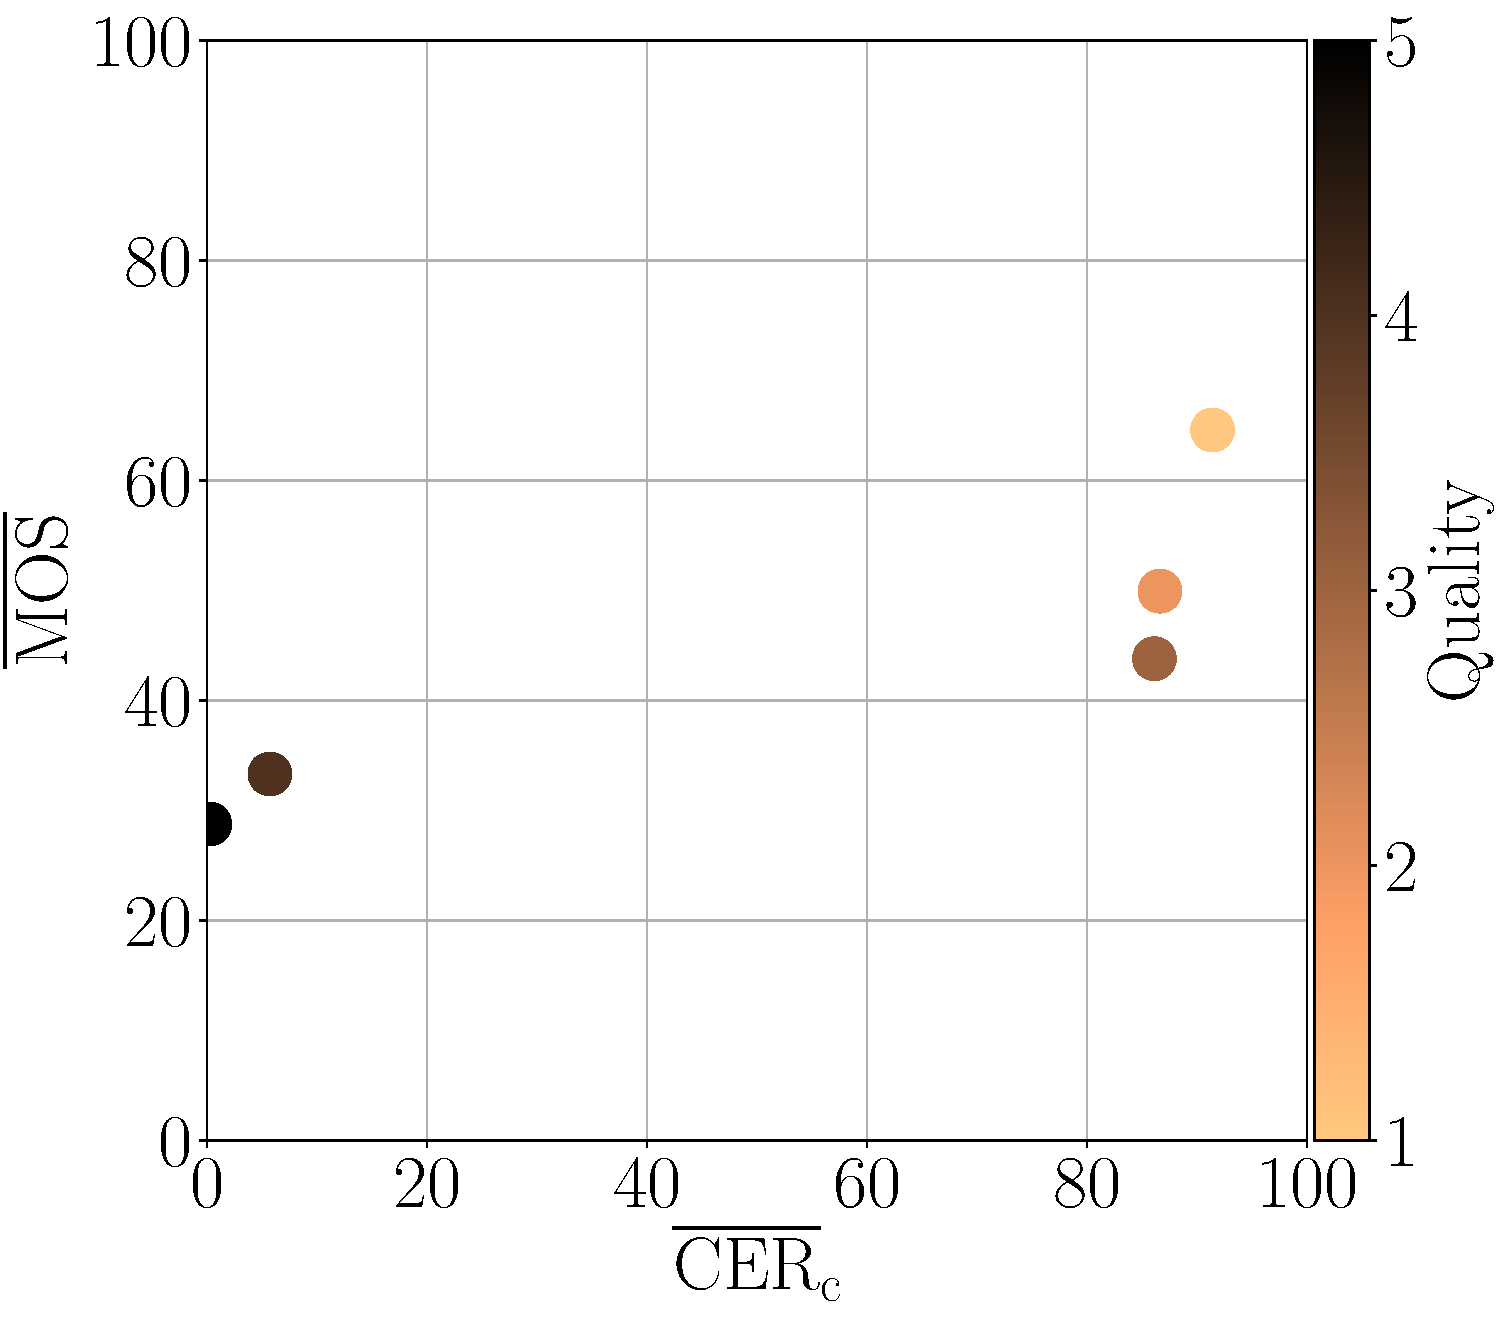
\includegraphics[width=\textwidth]{../../images/analyze/mos_cer_ref_mean_tess_GN.pdf}
        \caption{GN}
        \label{fig:mos_cer_ref_mean_tess_GN}
    \end{subfigure}
    \hfill
    \begin{subfigure}[b]{0.3\textwidth}
        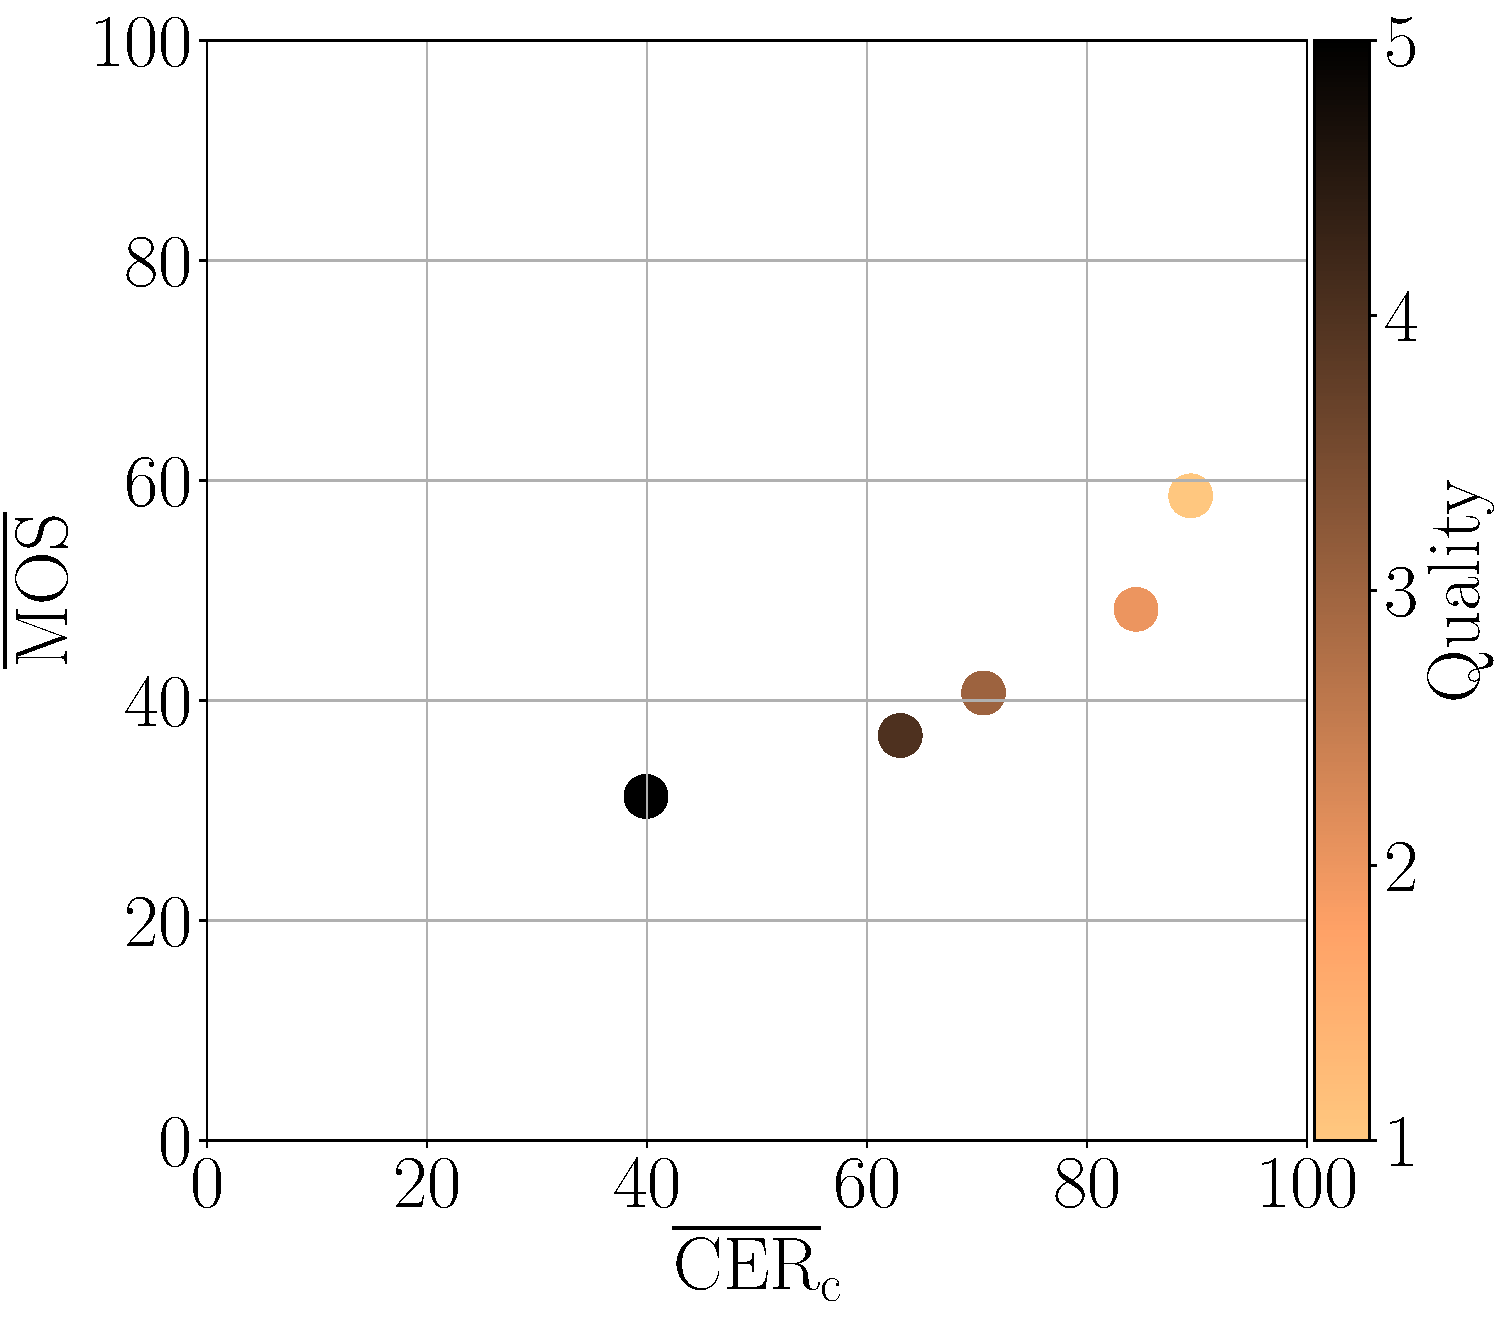
\includegraphics[width=\textwidth]{../../images/analyze/mos_cer_ref_mean_tess_GB.pdf}
        \caption{GB}
        \label{fig:mos_cer_ref_mean_tess_GB}
    \end{subfigure}
    \hfill
    \begin{subfigure}[b]{0.3\textwidth}
        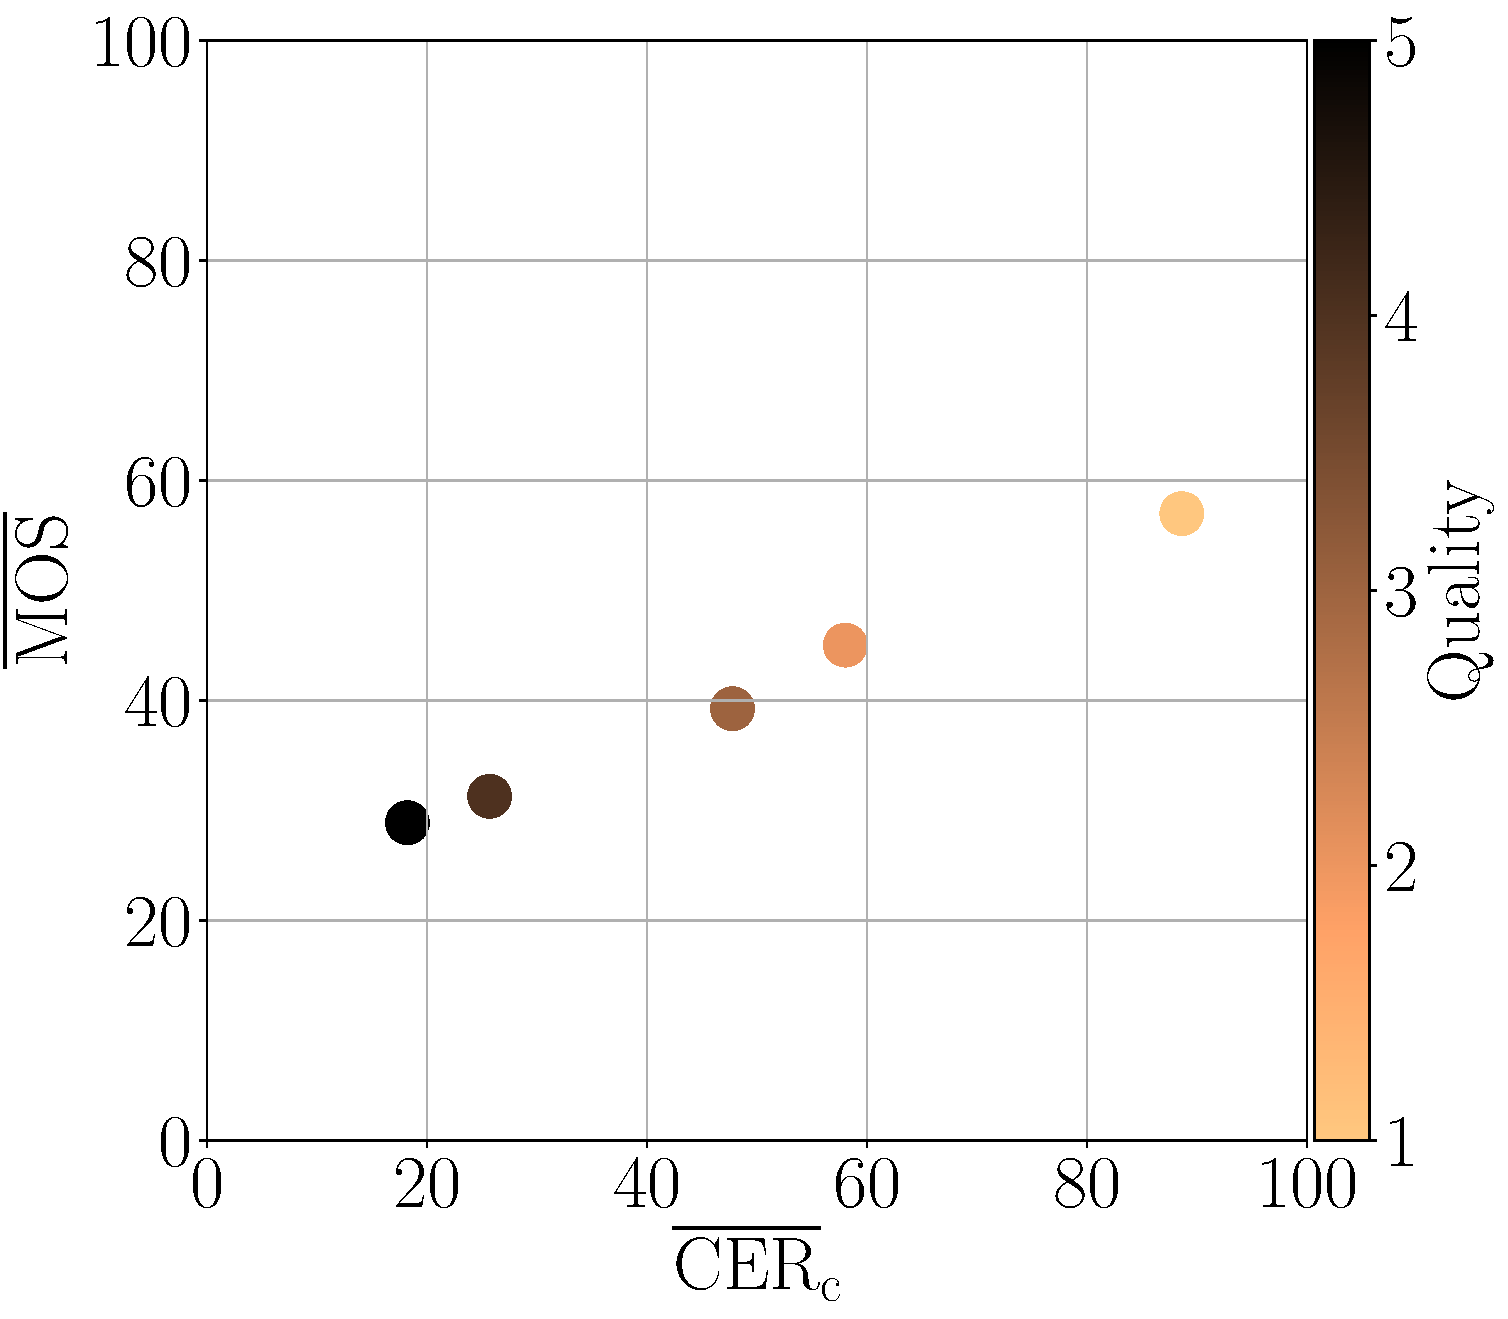
\includegraphics[width=\textwidth]{../../images/analyze/mos_cer_ref_mean_tess_MB.pdf}
        \caption{MB}
        \label{fig:mos_cer_ref_mean_tess_MB}
    \end{subfigure}
    \newline
    \begin{subfigure}[b]{0.3\textwidth}
        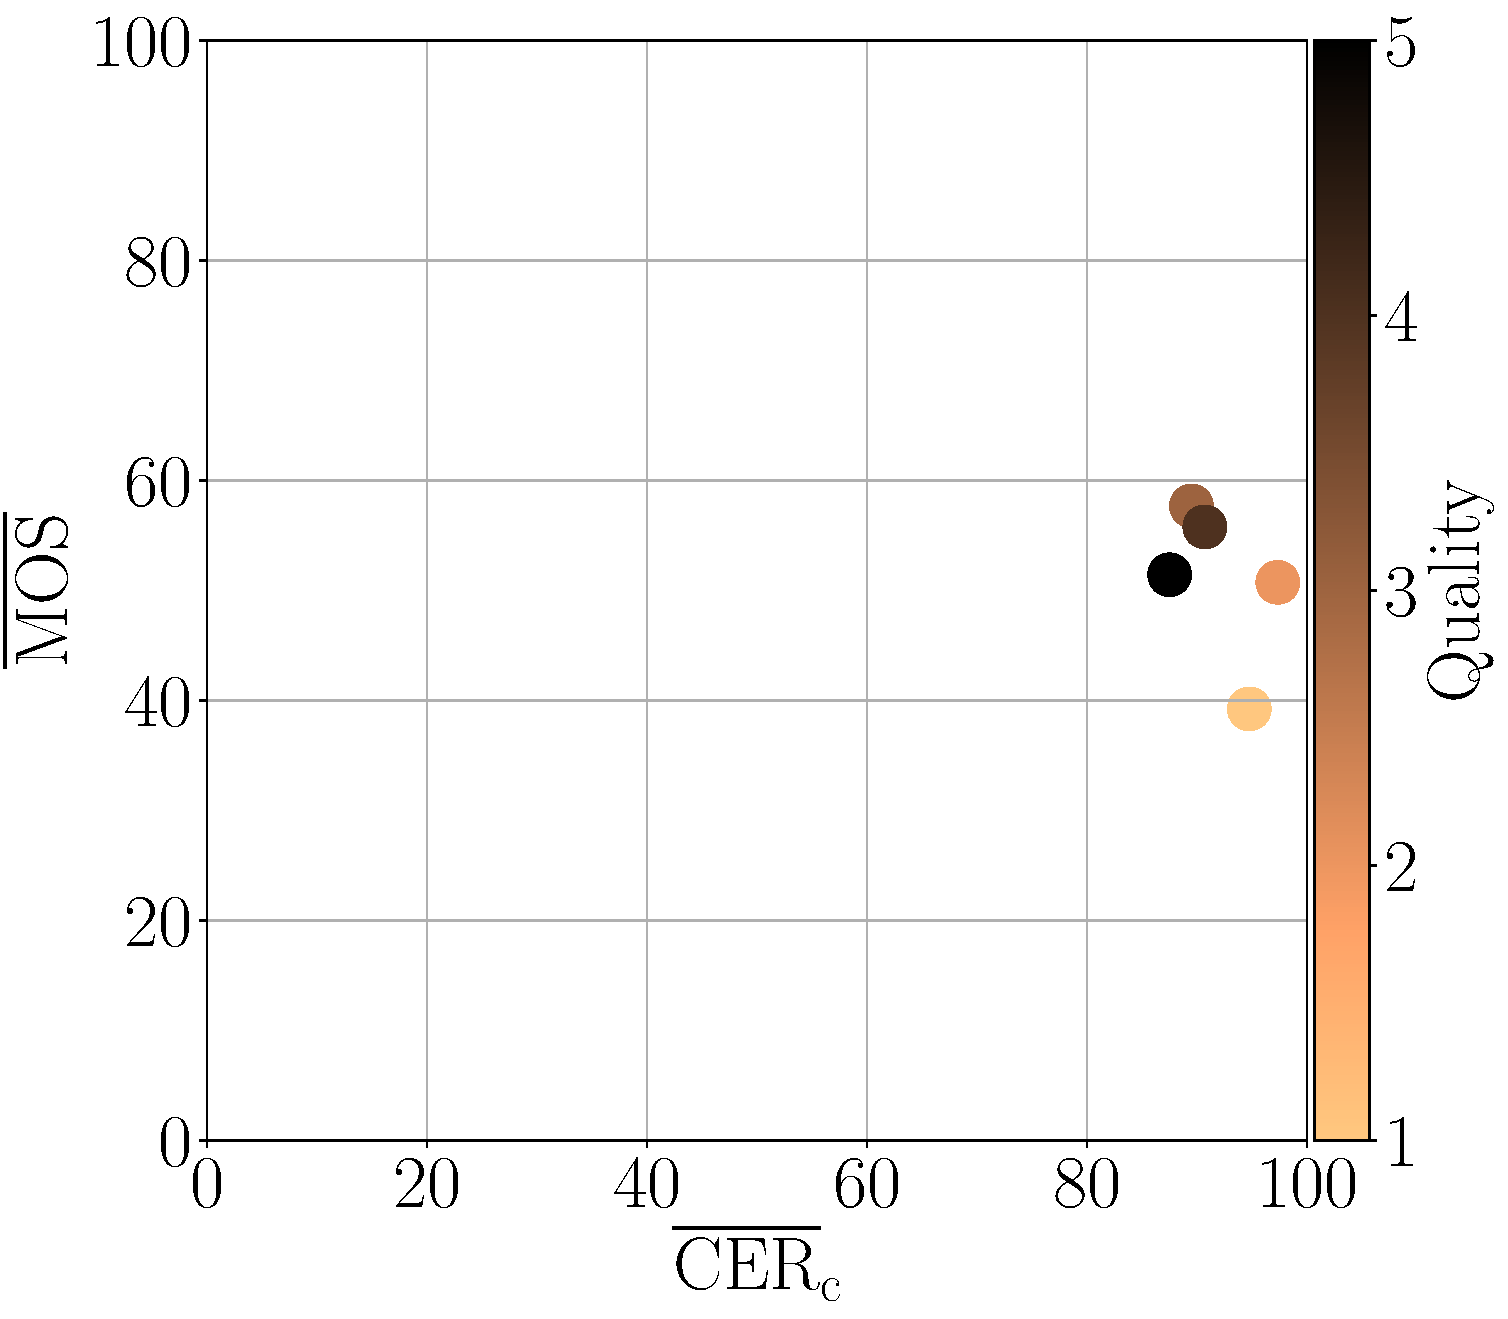
\includegraphics[width=\textwidth]{../../images/analyze/mos_cer_ref_mean_tess_CC.pdf}
        \caption{CC}
        \label{fig:mos_cer_ref_mean_tess_CC}
    \end{subfigure}
    \hfill
    \begin{subfigure}[b]{0.3\textwidth}
        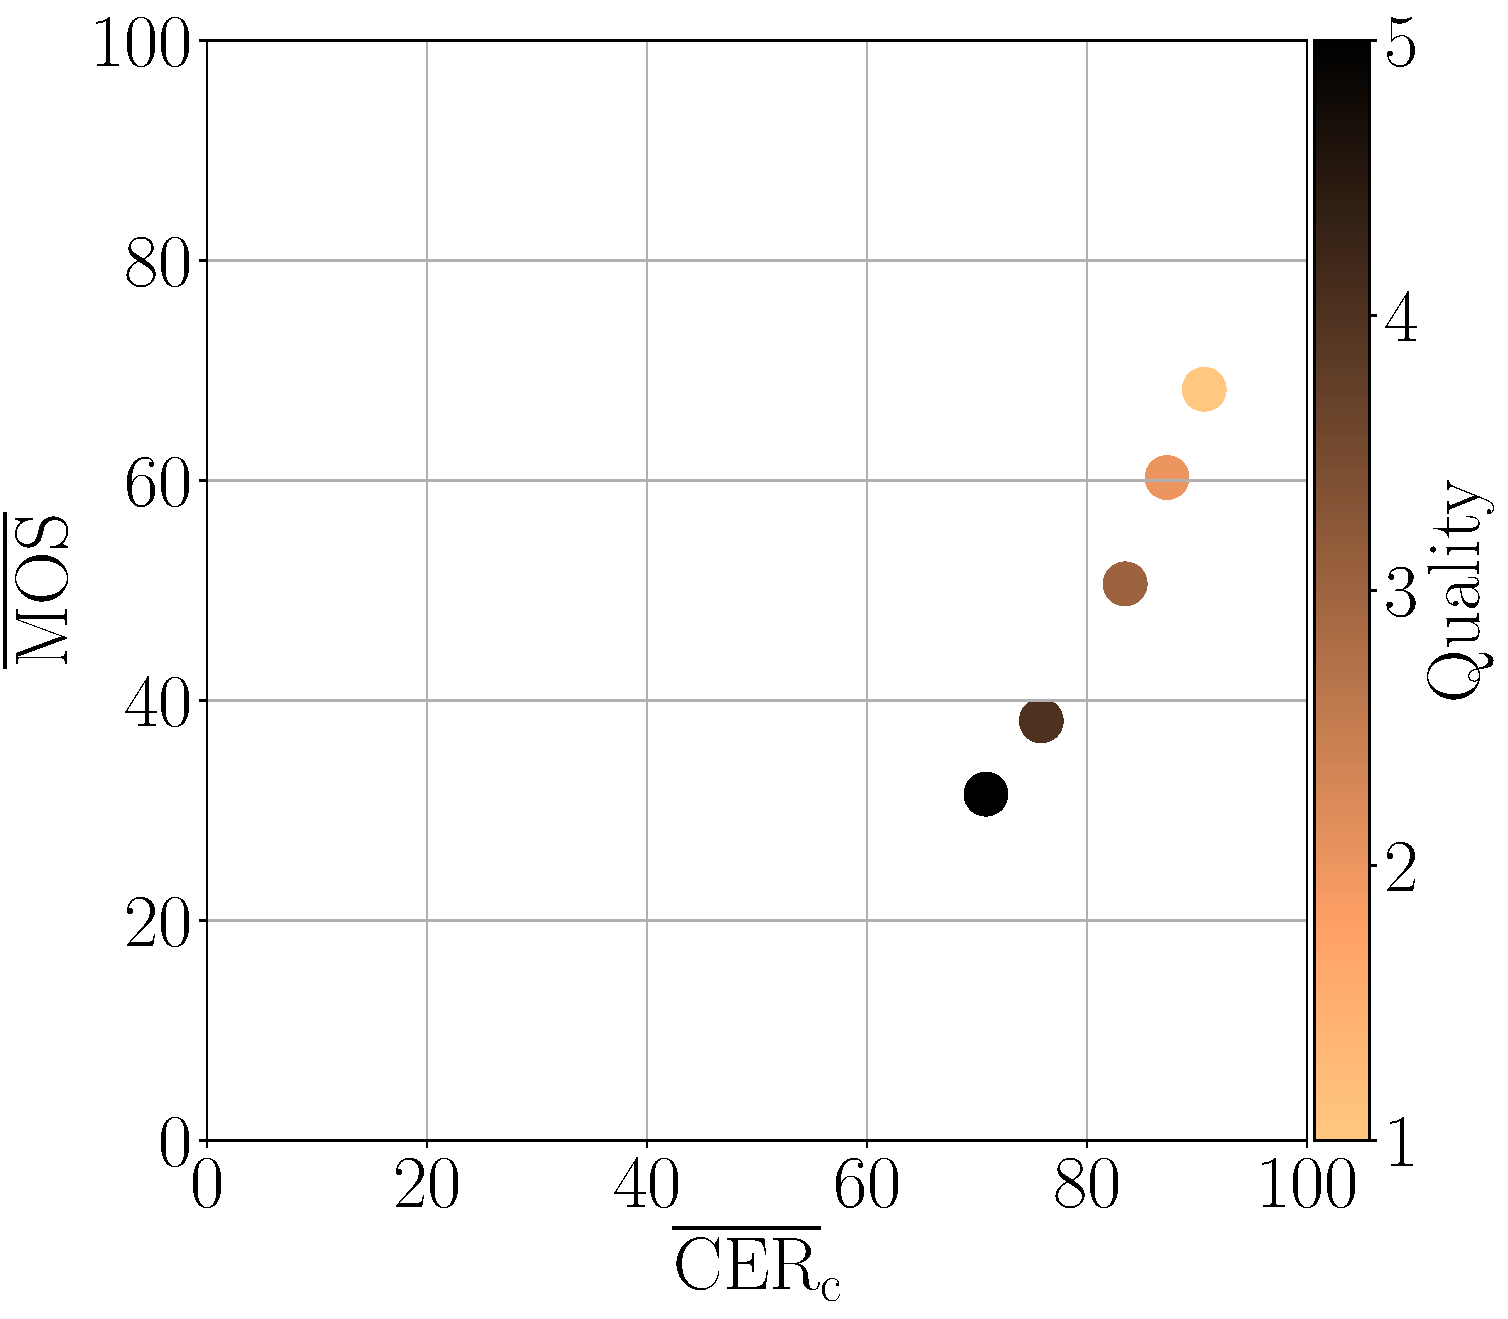
\includegraphics[width=\textwidth]{../../images/analyze/mos_cer_ref_mean_tess_JPEG.pdf}
        \caption{JPEG}
        \label{fig:mos_cer_ref_mean_tess_JPEG}
    \end{subfigure}
    \hfill
    \begin{subfigure}[b]{0.3\textwidth}
        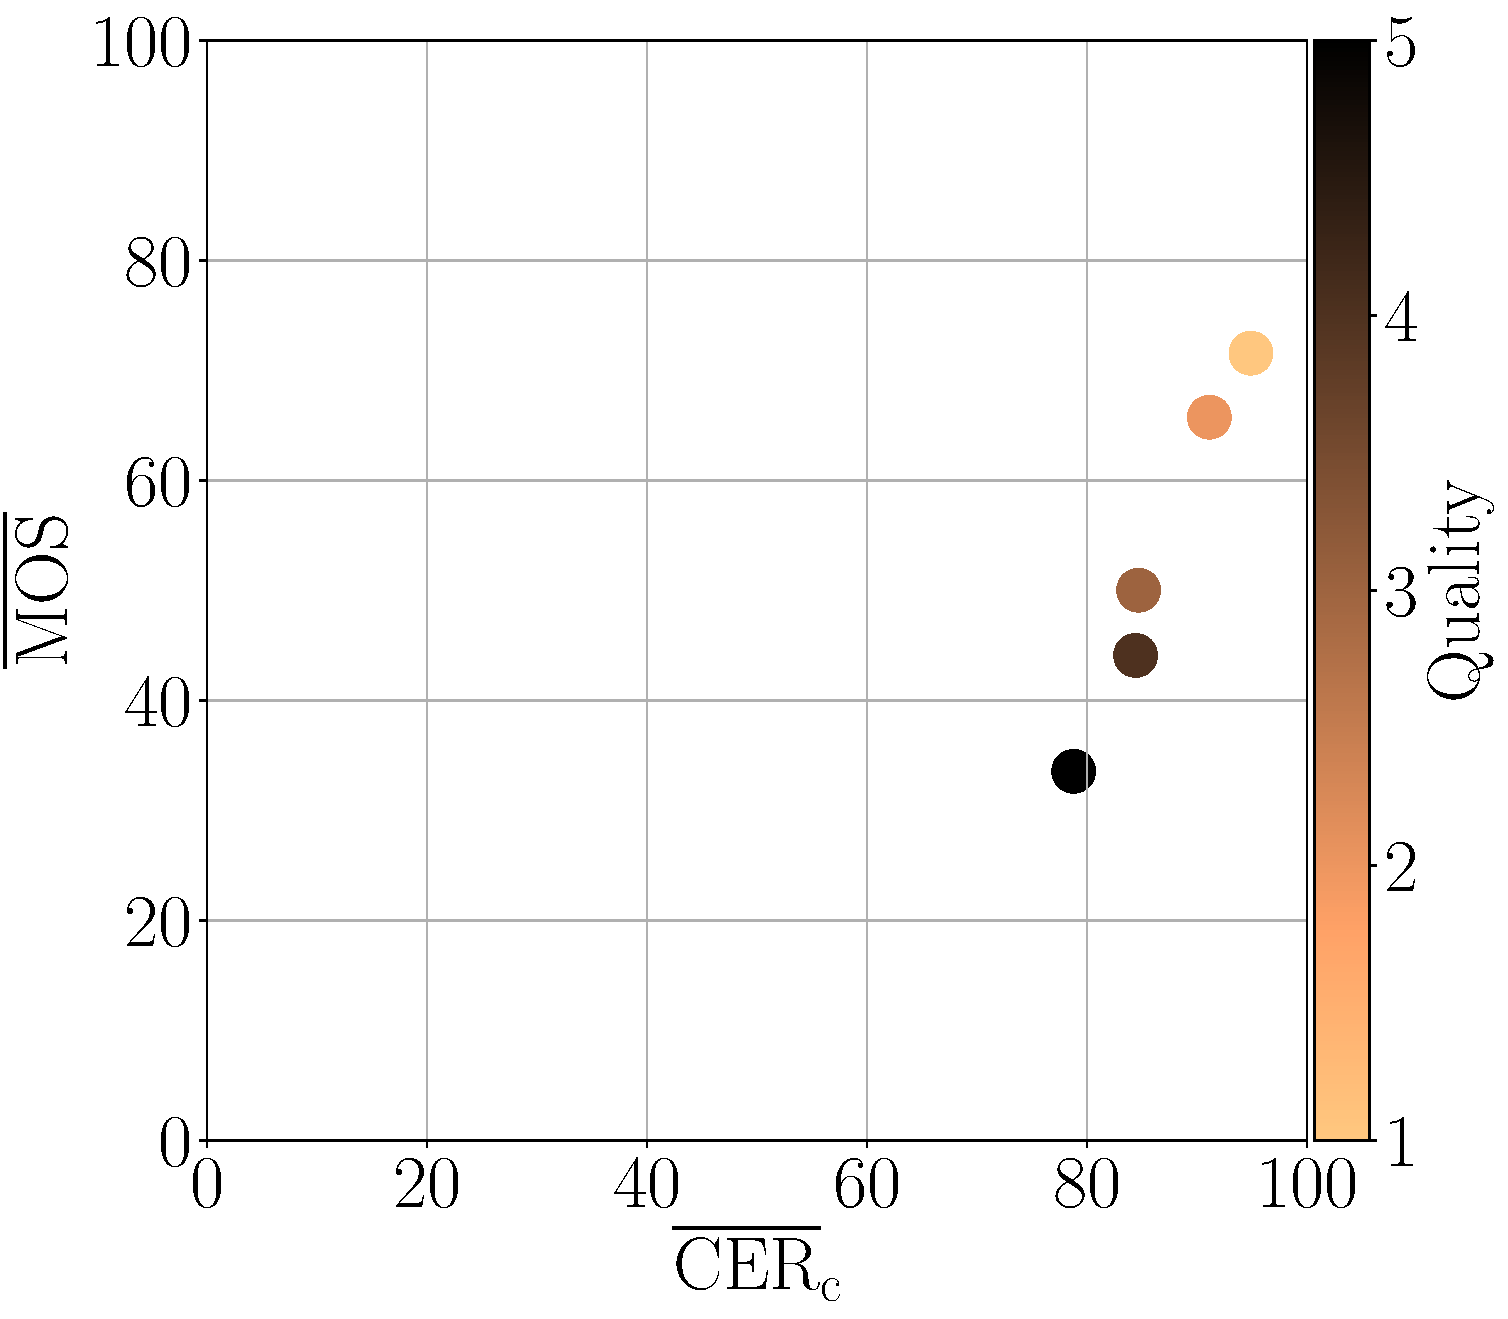
\includegraphics[width=\textwidth]{../../images/analyze/mos_cer_ref_mean_tess_JPEG2000.pdf}
        \caption{JPEG2000}
        \label{fig:mos_cer_ref_mean_tess_JPEG2000}
    \end{subfigure}
    \newline
    \begin{subfigure}[b]{0.3\textwidth}
        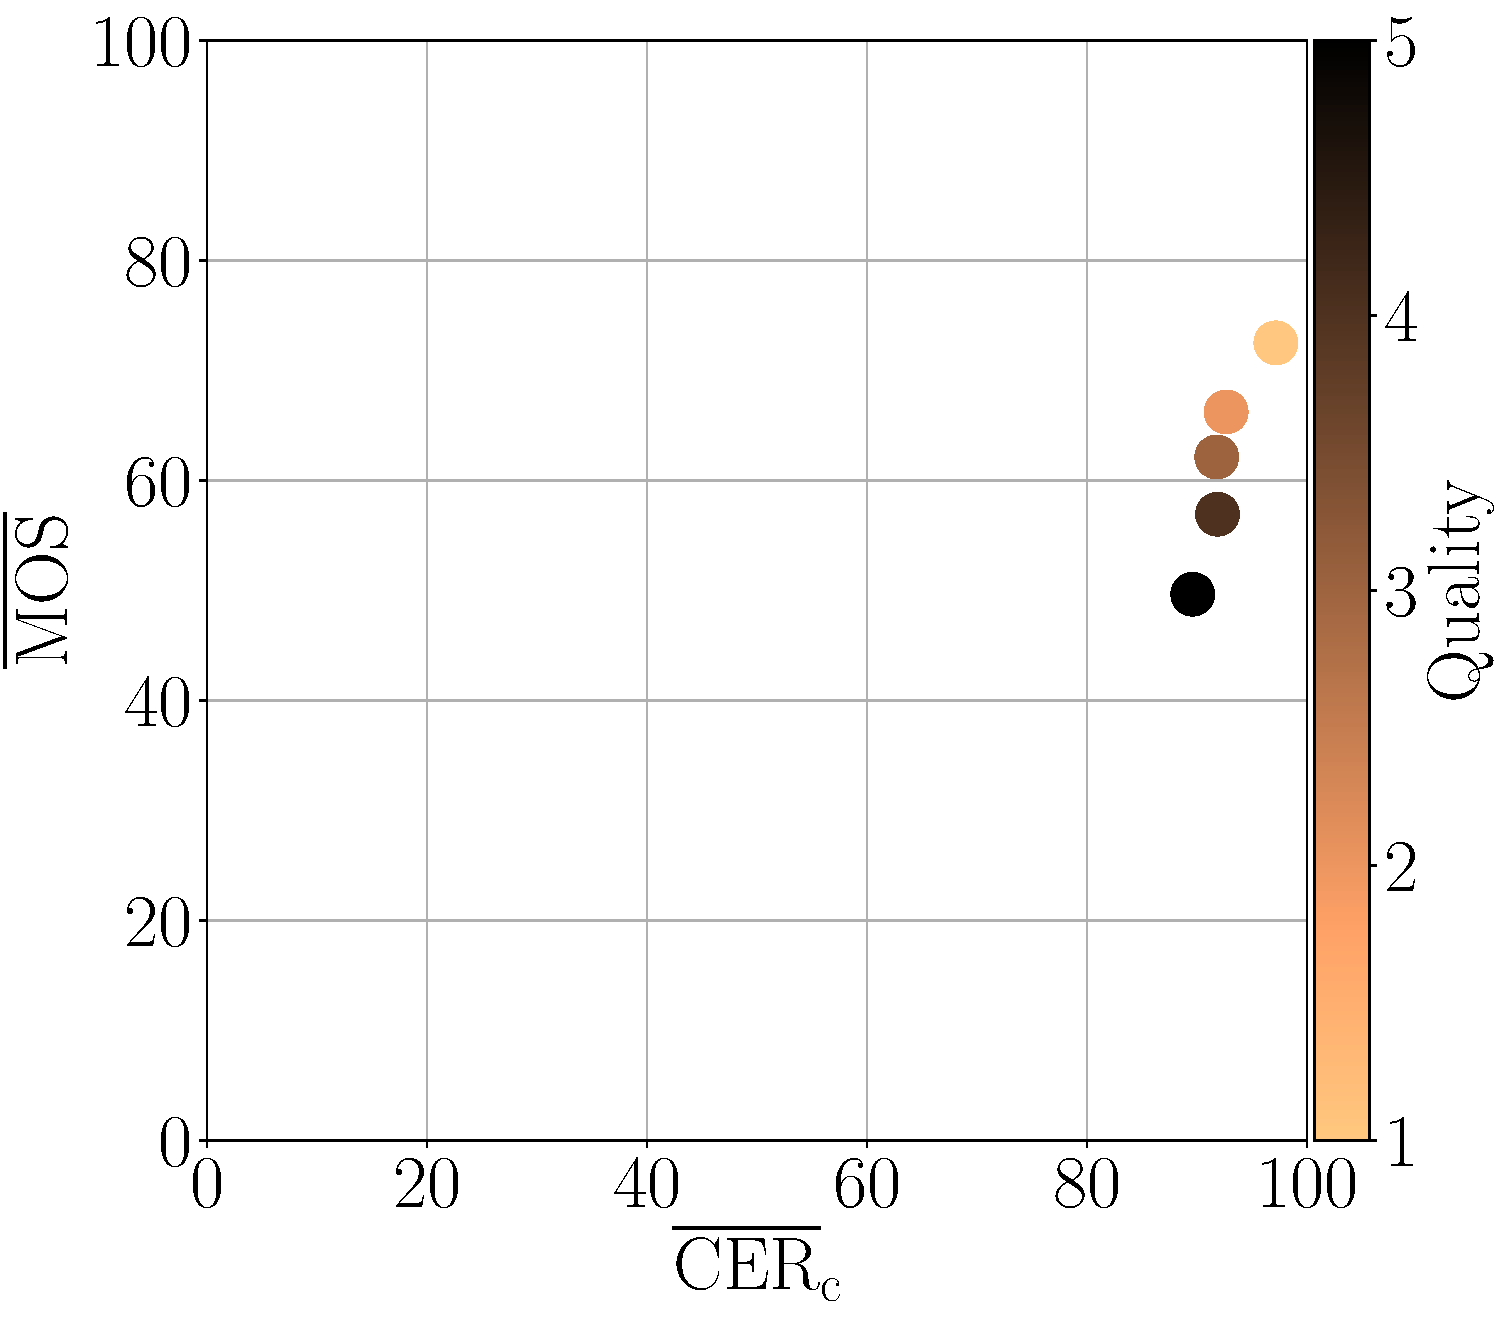
\includegraphics[width=\textwidth]{../../images/analyze/mos_cer_ref_mean_tess_CSC.pdf}
        \caption{CSC}
        \label{fig:mos_cer_ref_mean_tess_CSC}
    \end{subfigure}
    \hfill
    \begin{subfigure}[b]{0.3\textwidth}
        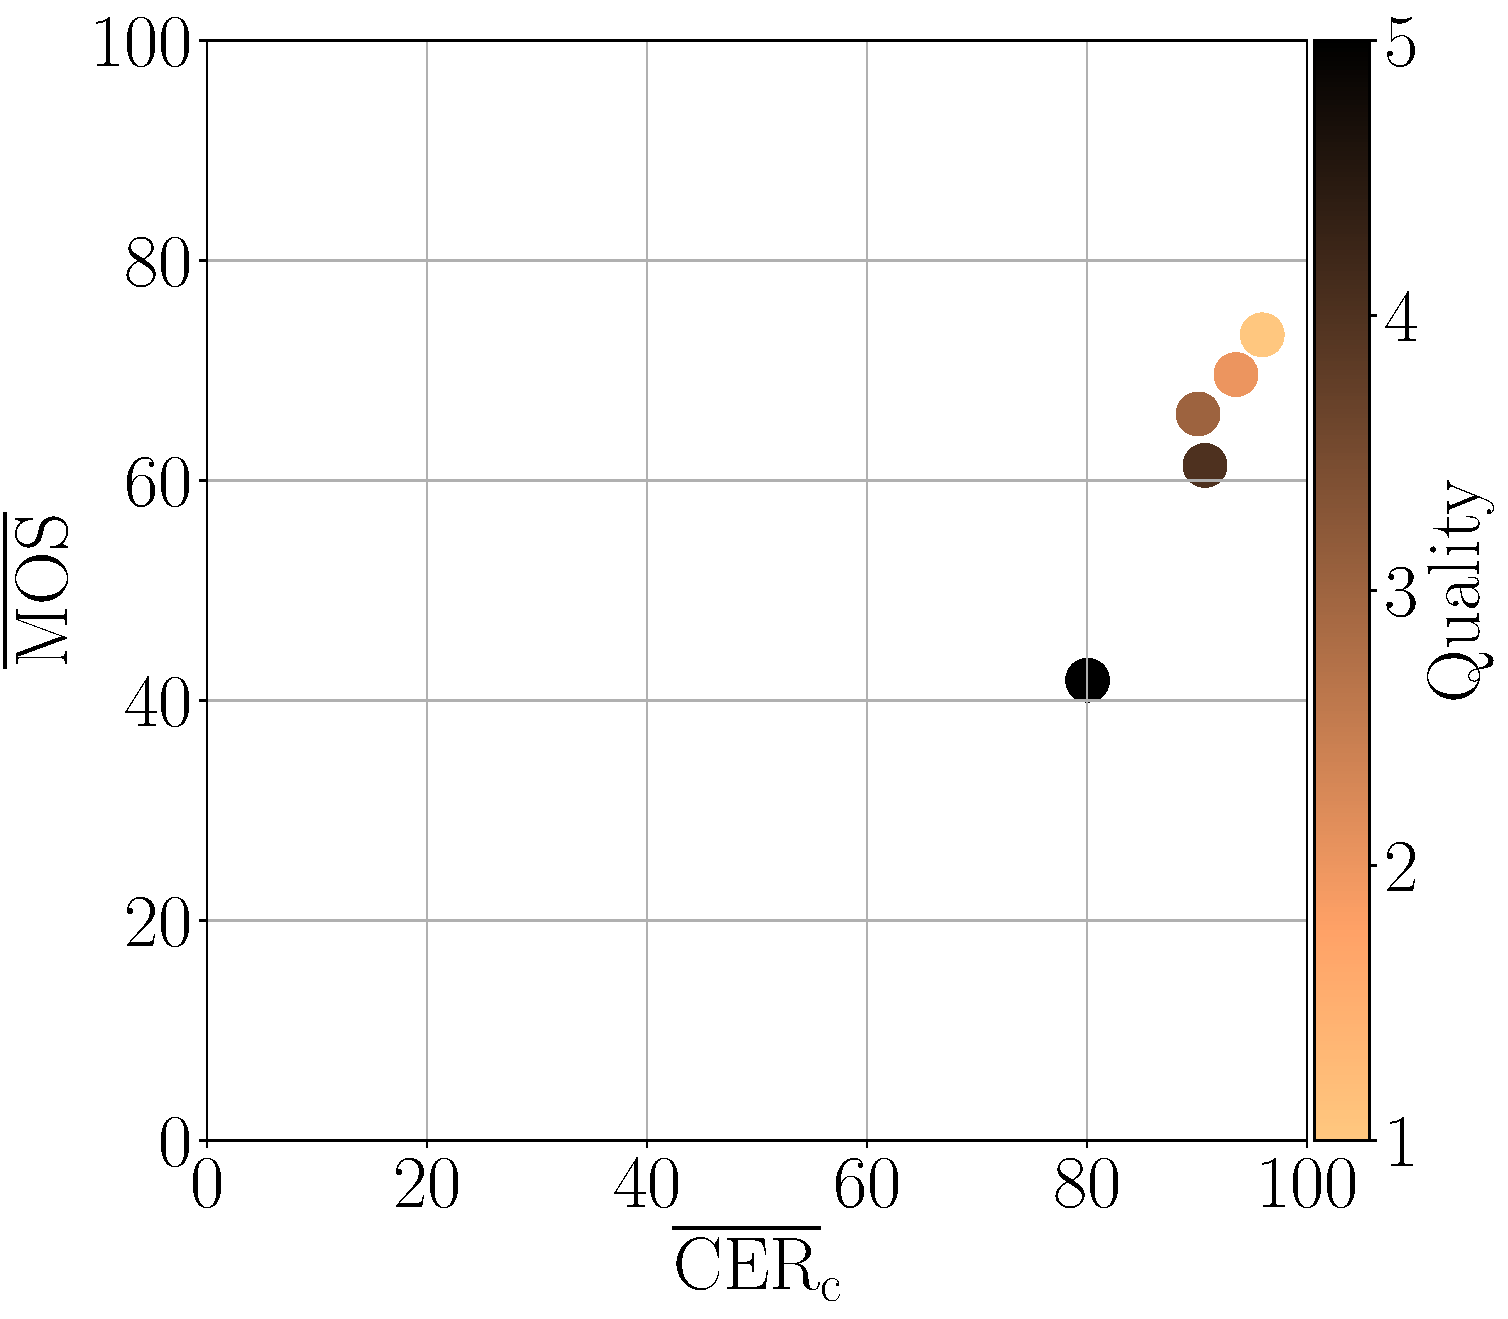
\includegraphics[width=\textwidth]{../../images/analyze/mos_cer_ref_mean_tess_HEVC-SCC.pdf}
        \caption{HEVC-SCC}
        \label{fig:mos_cer_ref_mean_tess_HEVC-SCC}
    \end{subfigure}
    \hfill
    \begin{subfigure}[b]{0.3\textwidth}
        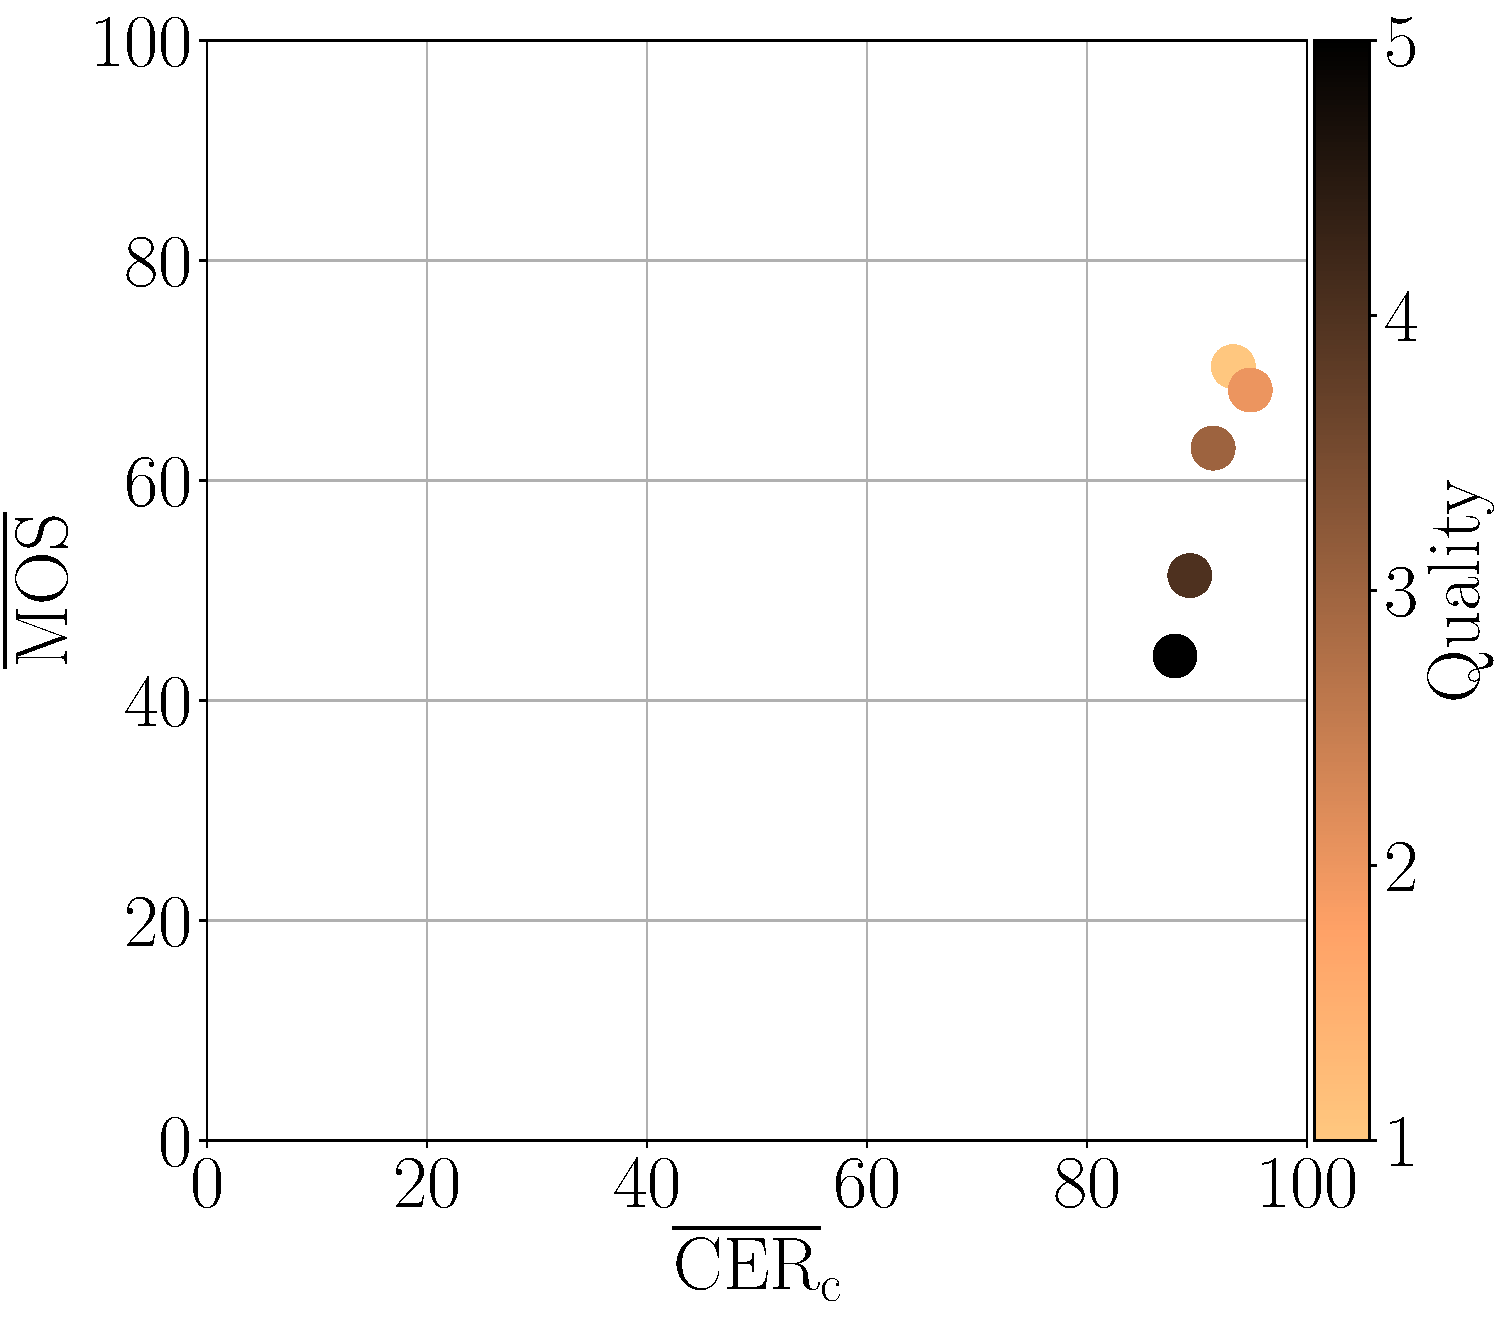
\includegraphics[width=\textwidth]{../../images/analyze/mos_cer_ref_mean_tess_CQD.pdf}
        \caption{CQD}
        \label{fig:mos_cer_ref_mean_tess_CQD}
    \end{subfigure}
    \caption{Mean \gls{cer} in relation to the reference against mean \gls{mos} for different distortion types with Tesseract \gls{ocr}.}
\label{fig:mos_cer_ref_mean_tess}
\end{figure}

In \autoref{fig:mos_cer_ref_mean_tess} we can see the mean \gls{cer} against the mean \gls{mos} over selected images for all distortions with Tesseract \gls{ocr}.


% mos vs cer (fitted) mean in relation to reference for ezocr
\begin{figure}[h]
\centering
    \begin{subfigure}[b]{0.3\textwidth}
        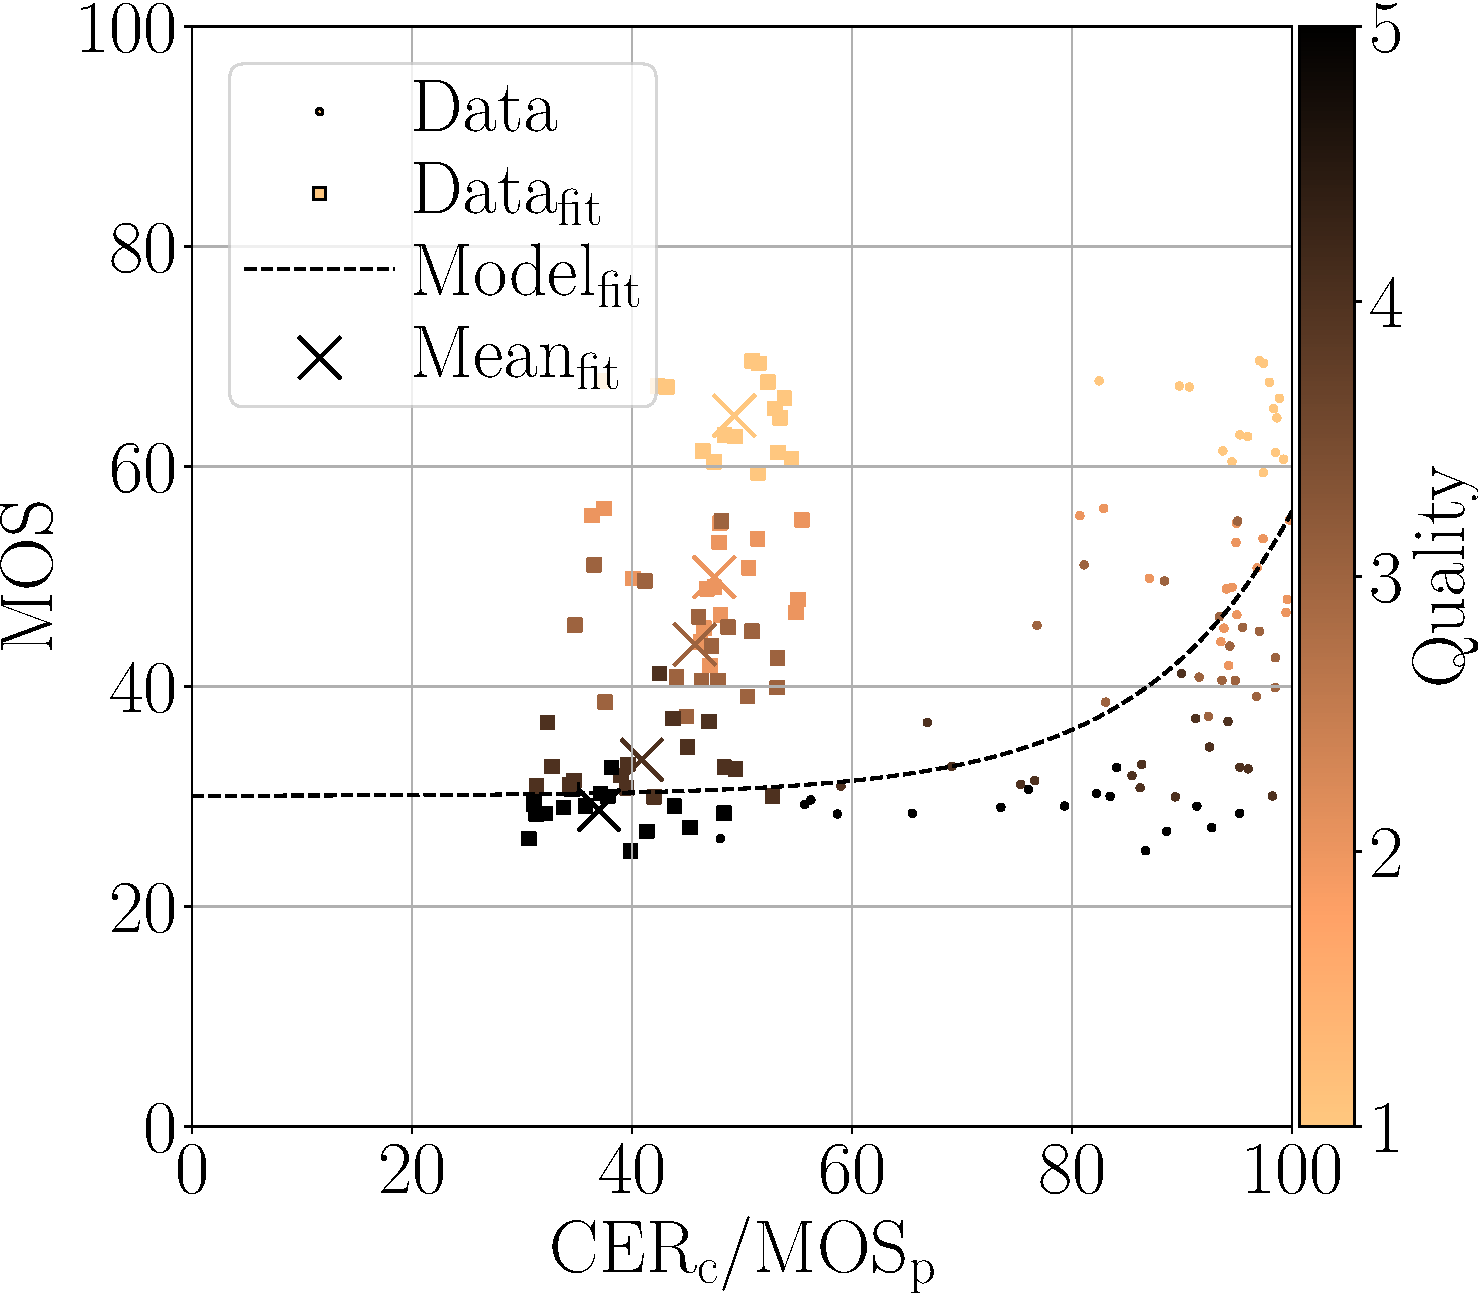
\includegraphics[width=\textwidth]{../../images/analyze/mos_cer_ref_fitted_mean_ezocr_GN.pdf}
        \caption{GN}
        \label{fig:mos_cer_ref_fitted_mean_ezocr_GN}
    \end{subfigure}
    \hfill
    \begin{subfigure}[b]{0.3\textwidth}
        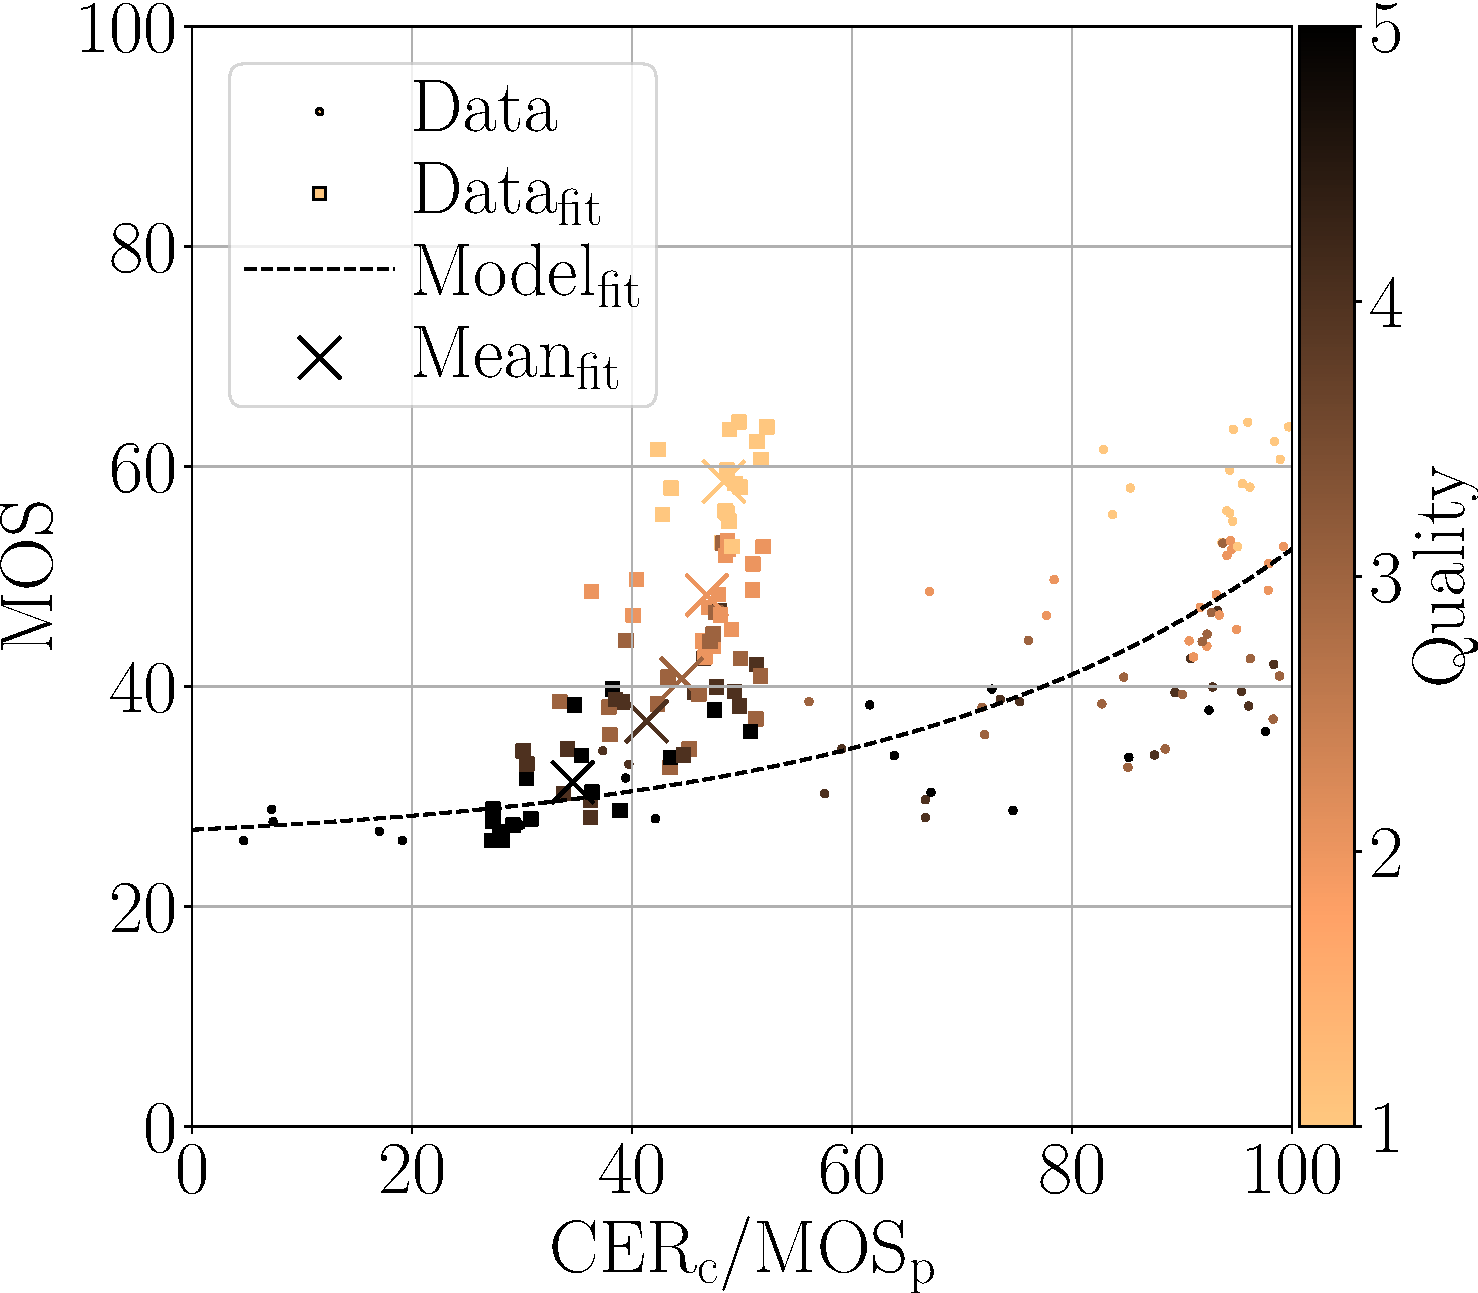
\includegraphics[width=\textwidth]{../../images/analyze/mos_cer_ref_fitted_mean_ezocr_GB.pdf}
        \caption{GB}
        \label{fig:mos_cer_ref_fitted_mean_ezocr_GB}
    \end{subfigure}
    \hfill
    \begin{subfigure}[b]{0.3\textwidth}
        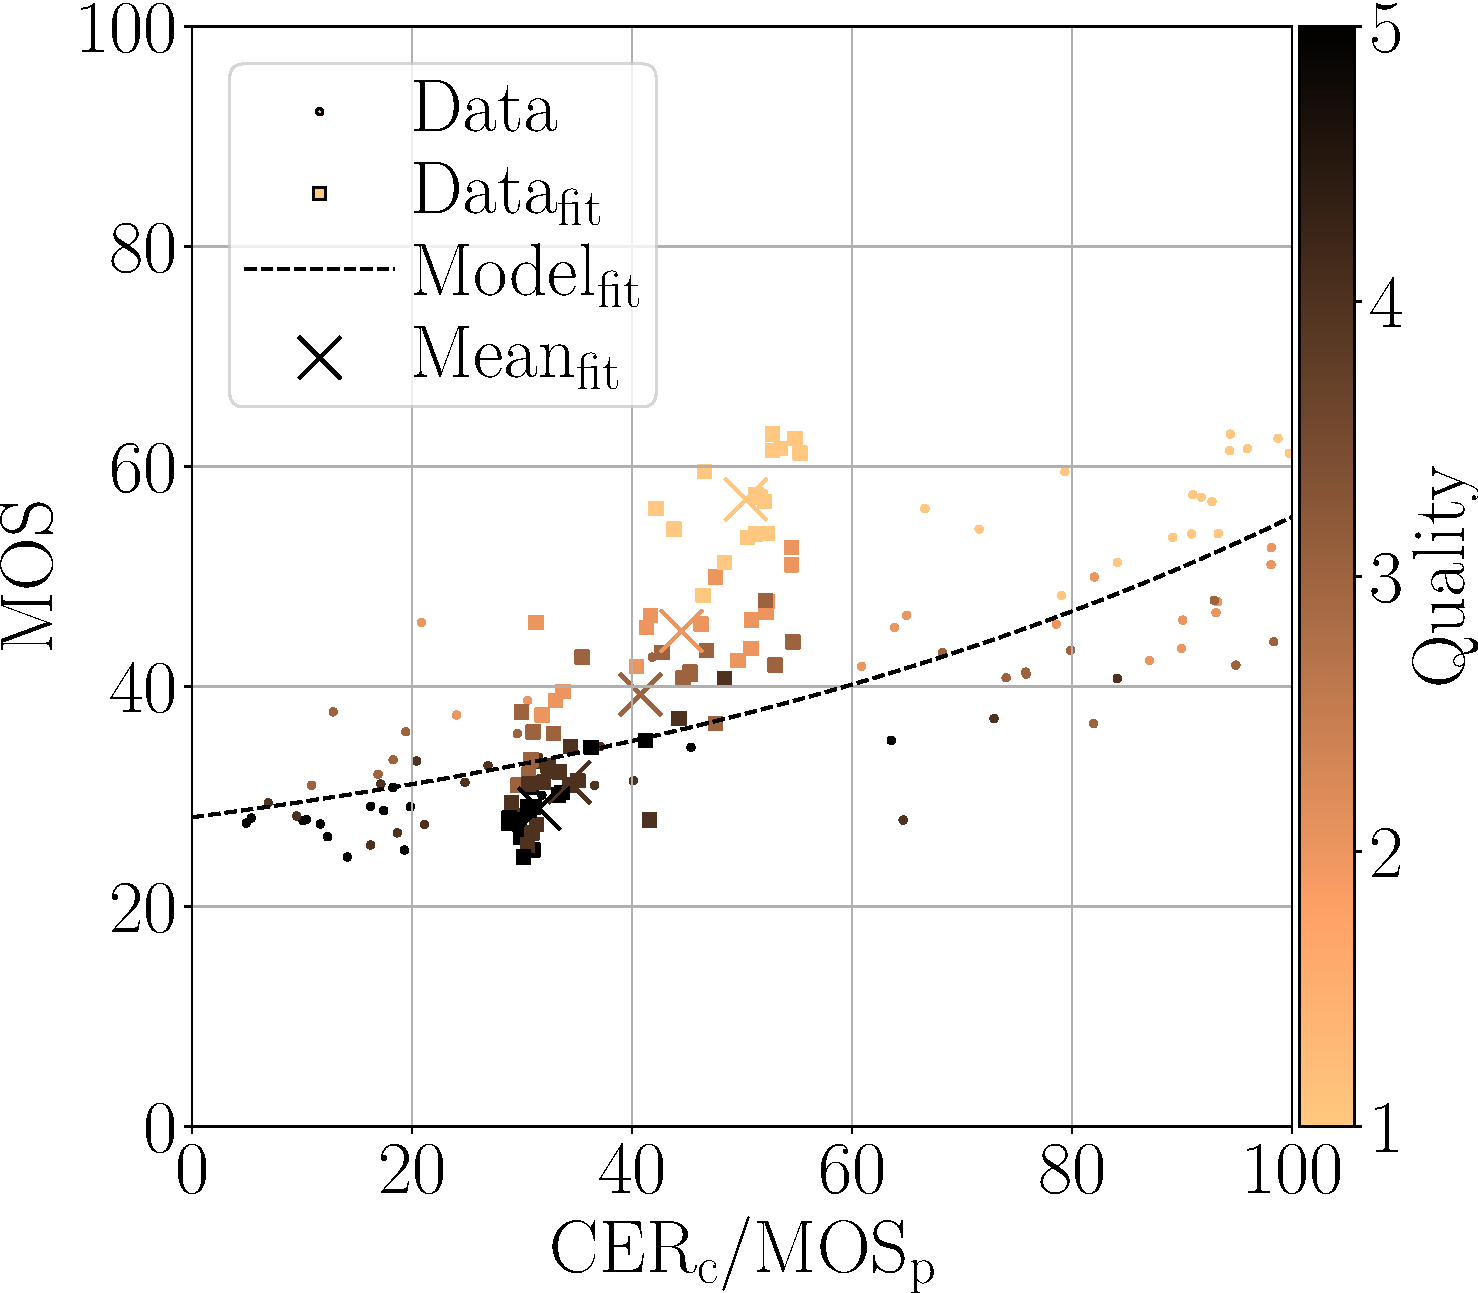
\includegraphics[width=\textwidth]{../../images/analyze/mos_cer_ref_fitted_mean_ezocr_MB.pdf}
        \caption{MB}
        \label{fig:mos_cer_ref_fitted_mean_ezocr_MB}
    \end{subfigure}
    \newline
    \begin{subfigure}[b]{0.3\textwidth}
        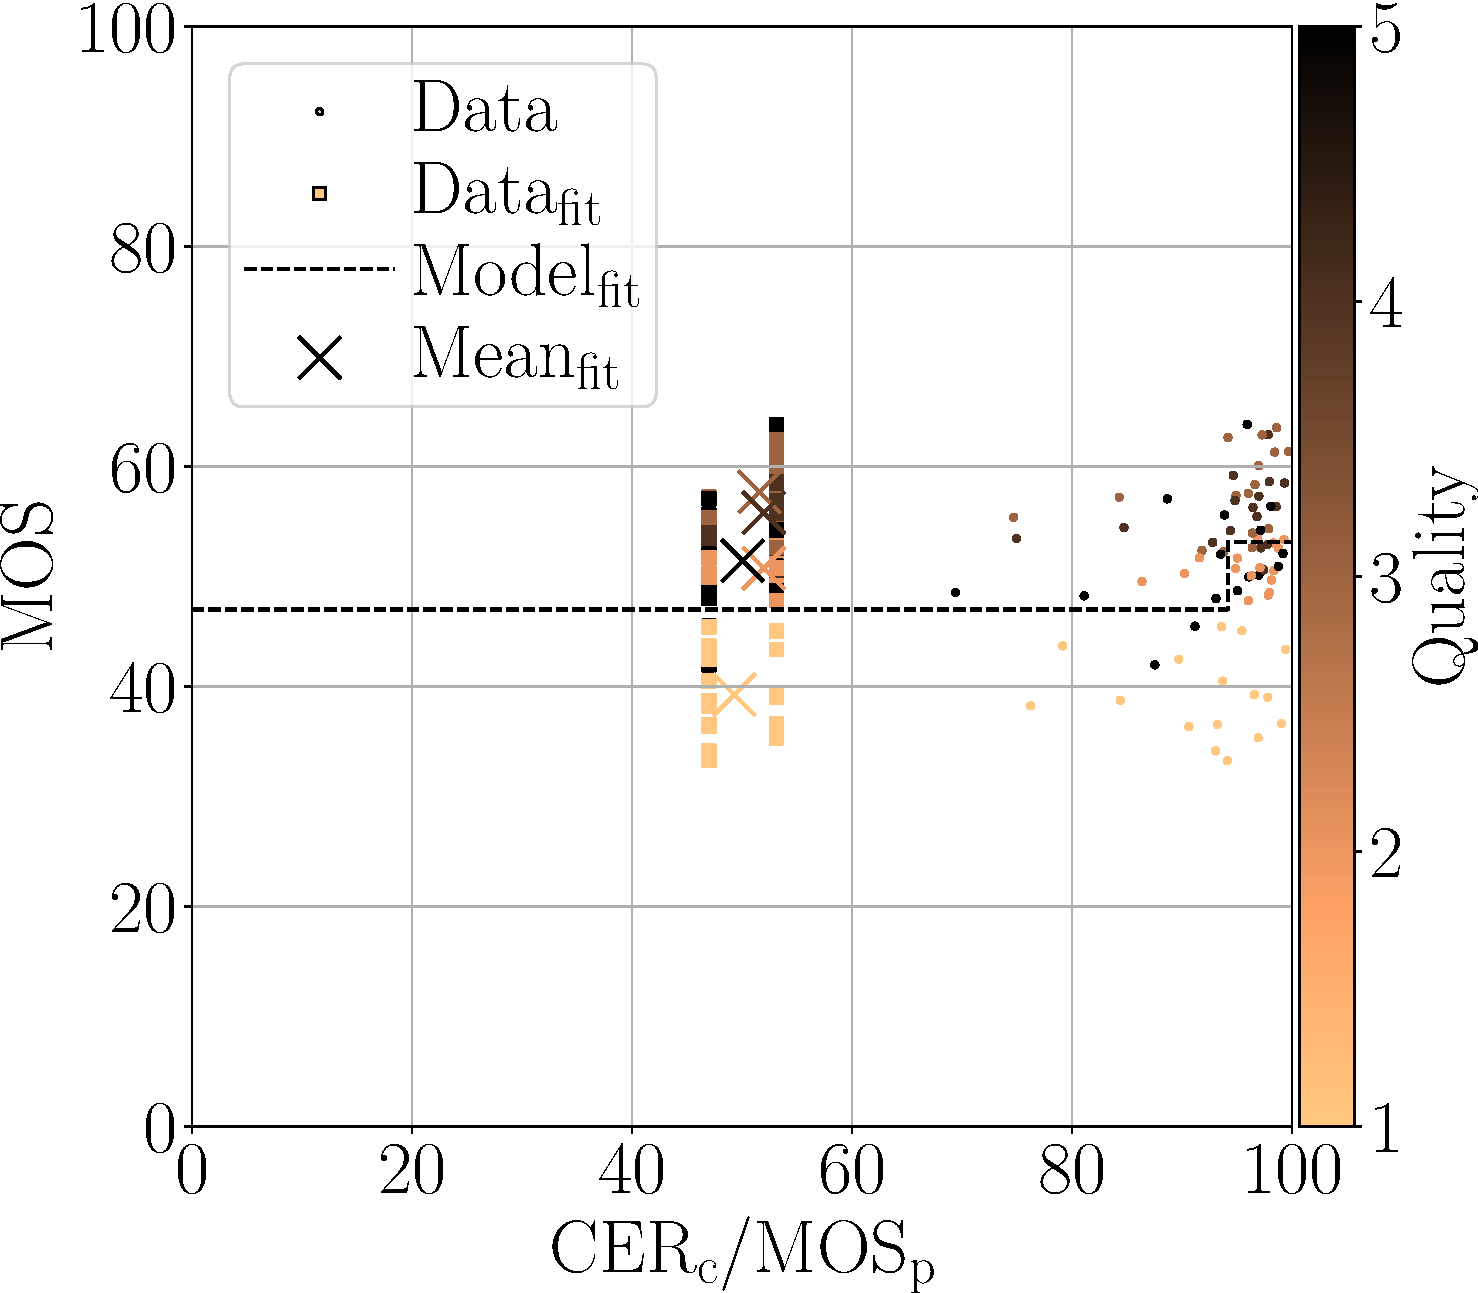
\includegraphics[width=\textwidth]{../../images/analyze/mos_cer_ref_fitted_mean_ezocr_CC.pdf}
        \caption{CC}
        \label{fig:mos_cer_ref_fitted_mean_ezocr_CC}
    \end{subfigure}
    \hfill
    \begin{subfigure}[b]{0.3\textwidth}
        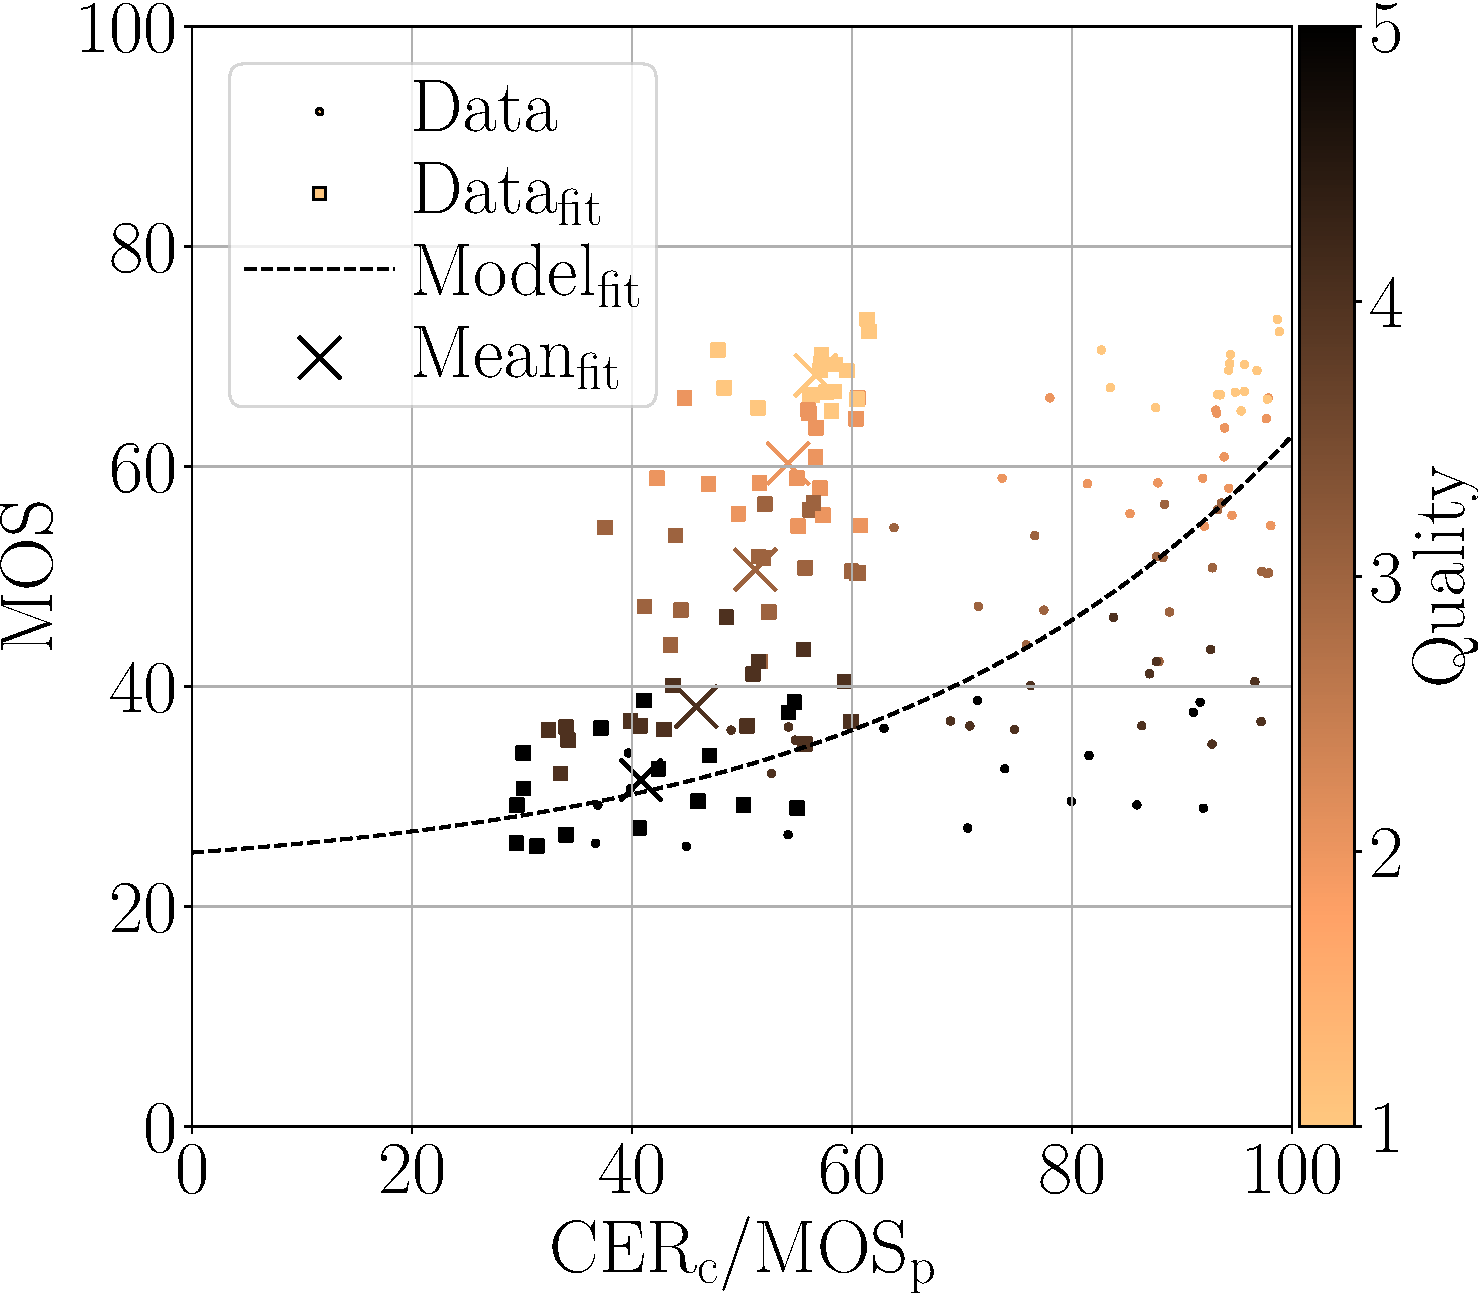
\includegraphics[width=\textwidth]{../../images/analyze/mos_cer_ref_fitted_mean_ezocr_JPEG.pdf}
        \caption{JPEG}
        \label{fig:mos_cer_ref_fitted_mean_ezocr_JPEG}
    \end{subfigure}
    \hfill
    \begin{subfigure}[b]{0.3\textwidth}
        \includegraphics[width=\textwidth]{../../images/analyze/mos_cer_ref_fitted_mean_ezocr_JPEG2000.pdf}
        \caption{JPEG2000}
        \label{fig:mos_cer_ref_fitted_mean_ezocr_JPEG2000}
    \end{subfigure}
    \newline
    \begin{subfigure}[b]{0.3\textwidth}
        \includegraphics[width=\textwidth]{../../images/analyze/mos_cer_ref_fitted_mean_ezocr_CSC.pdf}
        \caption{CSC}
        \label{fig:mos_cer_ref_fitted_mean_ezocr_CSC}
    \end{subfigure}
    \hfill
    \begin{subfigure}[b]{0.3\textwidth}
        \includegraphics[width=\textwidth]{../../images/analyze/mos_cer_ref_fitted_mean_ezocr_HEVC-SCC.pdf}
        \caption{HEVC-SCC}
        \label{fig:mos_cer_ref_fitted_mean_ezocr_HEVC-SCC}
    \end{subfigure}
    \hfill
    \begin{subfigure}[b]{0.3\textwidth}
        \includegraphics[width=\textwidth]{../../images/analyze/mos_cer_ref_fitted_mean_ezocr_CQD.pdf}
        \caption{CQD}
        \label{fig:mos_cer_ref_fitted_mean_ezocr_CQD}
    \end{subfigure}
    \caption{Mean \gls{cer} (fitted) in relation to the reference against mean \gls{mos} for different distortion types with EasyOCR.}
\label{fig:mos_cer_ref_fitted_mean_ezocr}
\end{figure}

In \autoref{fig:mos_cer_ref_fitted_mean_ezocr} we can see the mean \gls{cer} (fitted) against the mean \gls{mos} over selected images for all distortions with EasyOCR.

% mos vs cer (fitted) mean in relation to reference for Tesseract
\begin{figure}[h]
\centering
    \begin{subfigure}[b]{0.3\textwidth}
        \includegraphics[width=\textwidth]{../../images/analyze/mos_cer_ref_fitted_mean_tess_GN.pdf}
        \caption{GN}
        \label{fig:mos_cer_ref_fitted_mean_tess_GN}
    \end{subfigure}
    \hfill
    \begin{subfigure}[b]{0.3\textwidth}
        \includegraphics[width=\textwidth]{../../images/analyze/mos_cer_ref_fitted_mean_tess_GB.pdf}
        \caption{GB}
        \label{fig:mos_cer_ref_fitted_mean_tess_GB}
    \end{subfigure}
    \hfill
    \begin{subfigure}[b]{0.3\textwidth}
        \includegraphics[width=\textwidth]{../../images/analyze/mos_cer_ref_fitted_mean_tess_MB.pdf}
        \caption{MB}
        \label{fig:mos_cer_ref_fitted_mean_tess_MB}
    \end{subfigure}
    \newline
    \begin{subfigure}[b]{0.3\textwidth}
        \includegraphics[width=\textwidth]{../../images/analyze/mos_cer_ref_fitted_mean_tess_CC.pdf}
        \caption{CC}
        \label{fig:mos_cer_ref_fitted_mean_tess_CC}
    \end{subfigure}
    \hfill
    \begin{subfigure}[b]{0.3\textwidth}
        \includegraphics[width=\textwidth]{../../images/analyze/mos_cer_ref_fitted_mean_tess_JPEG.pdf}
        \caption{JPEG}
        \label{fig:mos_cer_ref_fitted_mean_tess_JPEG}
    \end{subfigure}
    \hfill
    \begin{subfigure}[b]{0.3\textwidth}
        \includegraphics[width=\textwidth]{../../images/analyze/mos_cer_ref_fitted_mean_tess_JPEG2000.pdf}
        \caption{JPEG2000}
        \label{fig:mos_cer_ref_fitted_mean_tess_JPEG2000}
    \end{subfigure}
    \newline
    \begin{subfigure}[b]{0.3\textwidth}
        \includegraphics[width=\textwidth]{../../images/analyze/mos_cer_ref_fitted_mean_tess_CSC.pdf}
        \caption{CSC}
        \label{fig:mos_cer_ref_fitted_mean_tess_CSC}
    \end{subfigure}
    \hfill
    \begin{subfigure}[b]{0.3\textwidth}
        \includegraphics[width=\textwidth]{../../images/analyze/mos_cer_ref_fitted_mean_tess_HEVC-SCC.pdf}
        \caption{HEVC-SCC}
        \label{fig:mos_cer_ref_fitted_mean_tess_HEVC-SCC}
    \end{subfigure}
    \hfill
    \begin{subfigure}[b]{0.3\textwidth}
        \includegraphics[width=\textwidth]{../../images/analyze/mos_cer_ref_fitted_mean_tess_CQD.pdf}
        \caption{CQD}
        \label{fig:mos_cer_ref_fitted_mean_tess_CQD}
    \end{subfigure}
    \caption{Mean \gls{cer} (fitted) in relation to the reference against mean \gls{mos} for different distortion types with Tesseract \gls{ocr}.}
\label{fig:mos_cer_ref_fitted_mean_tess}
\end{figure}

In \autoref{fig:mos_cer_ref_fitted_mean_tess} we can see the mean \gls{cer} (fitted) against the mean \gls{mos} over selected images for all distortions with Tesseract \gls{ocr}.

\begin{table}[h]
\centering
\begin{tabular}{llrrrr}
\toprule
          & {} & \multicolumn{4}{l}{CER\_comp} \\
          & ocr\_algo & \multicolumn{2}{l}{ezocr} & \multicolumn{2}{l}{tess} \\
          & target &       gt &   ref &    gt &   ref \\
corr & dist\_name &          &       &       &       \\
\midrule
pearson & CC &     0.01 &  0.37 & -0.19 & -0.48 \\
          & CQD &     0.25 &  0.86 & -0.02 &  0.49 \\
          & CSC &     0.27 &  0.78 &  0.03 &  0.53 \\
          & GB &     0.57 &  0.80 &  0.39 &  0.69 \\
          & GN &     0.50 &  0.81 &  0.84 &  0.84 \\
          & HEVC-SCC &     0.57 &  0.92 &  0.41 &  0.68 \\
          & JPEG &     0.84 &  0.91 &  0.49 &  0.77 \\
          & JPEG2000 &     0.54 &  0.82 &  0.52 &  0.72 \\
          & MB &     0.89 &  0.90 &  0.77 &  0.82 \\
spearmanr & CC &     0.08 &  0.23 & -0.31 & -0.48 \\
          & CQD &     0.24 &  0.83 & -0.06 &  0.47 \\
          & CSC &     0.27 &  0.79 &  0.00 &  0.54 \\
          & GB &     0.70 &  0.96 &  0.45 &  0.73 \\
          & GN &     0.57 &  0.89 &  0.82 &  0.89 \\
          & HEVC-SCC &     0.46 &  0.85 &  0.31 &  0.54 \\
          & JPEG &     0.85 &  0.96 &  0.45 &  0.79 \\
          & JPEG2000 &     0.51 &  0.87 &  0.49 &  0.70 \\
          & MB &     0.93 &  0.94 &  0.80 &  0.80 \\
\bottomrule
\end{tabular}
\caption{Correlation between CER\_comp and MOS for different distortion types}
\label{tab:pearson_spear}
\end{table}

In \autoref{tab:pearson_spear} we can see the correlation between the \gls{cer}, in relation to the \gls{gt} and the reference, and the \gls{mos} for all distortions with EasyOCR and Tesseract \gls{ocr}.
We can generally observe that the correlation is higher for the \gls{cer} in relation to the reference compared to the \gls{gt}.
This might be due to the fact that the \gls{ocr} sometimes predicts text where there is no text or the \gls{gt} does not contain that text.
Thus when the quality gets worse, it might happen, that those text elements do not get predicted at all, thus resulting in a better performance.
The correlation is affected because the \gls{cer} first goes up and then down again, but the \gls{mos} is strictly decreasing.

The \gls{plcc} is generally higher for EasyOCR than for Tesseract \gls{ocr}.
This suggests that EasyOCR is more similarly to humans than Tesseract \gls{ocr} with regard to the impact on the \gls{cer} by the distortions.
Additionally the lowest \gls{plcc} is seen for \gls{cc}, which further confirms our assumption that \gls{cc} is not really an impact for the \gls{ocr} and thus not correlated with the \gls{mos}.
Similar observations, although more dominant for \gls{srcc}, can be made for \gls{csc} and \gls{cqd}.
These two distortions also seem to have more impact on the \gls{mos} than on the \gls{ocr} algorithms, which makes sense.


\begin{table}[h]
\centering
\begin{tabular}{llrrrr}
\toprule
                 & {} & \multicolumn{4}{l}{CER\_comp\_fitted} \\
                 & ocr\_algo & \multicolumn{2}{l}{ezocr} & \multicolumn{2}{l}{tess} \\
                 & target &              gt &   ref &    gt &   ref \\
corr & dist\_name &                 &       &       &       \\
\midrule
pearson\_fitted & CC &            0.98 &  0.89 &  0.99 & -0.98 \\
                 & CQD &           -0.91 &  0.92 &  0.99 &  0.99 \\
                 & CSC &           -1.00 &  0.87 &  0.96 &  0.96 \\
                 & GB &            0.99 &  0.98 &  1.00 &  1.00 \\
                 & GN &            0.93 &  0.98 &  0.99 &  0.99 \\
                 & HEVC-SCC &            0.83 &  1.00 &  0.90 &  0.86 \\
                 & JPEG &            0.98 &  0.99 &  0.88 &  1.00 \\
                 & JPEG2000 &            0.85 &  0.98 &  0.99 &  0.85 \\
                 & MB &            1.00 &  1.00 &  1.00 &  0.99 \\
spearmanr\_fitted & CC &            1.00 &  0.99 &  1.00 & -1.00 \\
                 & CQD &           -0.83 &  1.00 &  1.00 &  1.00 \\
                 & CSC &           -1.00 &  1.00 &  0.80 &  1.00 \\
                 & GB &            1.00 &  1.00 &  1.00 &  1.00 \\
                 & GN &            0.97 &  1.00 &  1.00 &  1.00 \\
                 & HEVC-SCC &            0.96 &  1.00 &  0.93 &  1.00 \\
                 & JPEG &            1.00 &  1.00 &  0.98 &  1.00 \\
                 & JPEG2000 &            0.97 &  1.00 &  1.00 &  0.94 \\
                 & MB &            1.00 &  1.00 &  1.00 &  1.00 \\
\bottomrule
\end{tabular}
    \caption{Correlation between $CER_{comp}$ (fitted) and MOS for different distortion types}
\label{tab:pearson_spear_fitted}
\end{table}

In \autoref{tab:pearson_spear} we can see the correlation between the \gls{cer}, in relation to the \gls{gt} and the reference, and the now fitted \gls{mos} values for all distortions with EasyOCR and Tesseract \gls{ocr}.
After fitting the \gls{mos} values, we can observe that the correlations increased across the whole table.
This is to be expected, since most of the fitted models are monotonic functions, which makes a higher \gls{cer} always result in a higher \gls{mos} or vice versa, when going along the model's curve.
The only exception is \gls{cc}, which shows a negative \gls{plcc} and \gls{srcc}.
This is due to a strictly decreasing fitted model as can be seen in \autoref{fig:mos_cer_ref_fitted_mean_tess_CC}.

In summary, we can say that the \gls{gn}, \gls{mb}, \gls{gb}, \gls{jpeg} and \gls{jpeg2000} distortions have a high correlation with the \gls{mos} and \gls{ocr} might be a useful alternative to human judgment.
However, for \gls{cc}, \gls{csc} and \gls{cqd} the correlation with the \gls{mos} is low and \gls{ocr} might not be a good alternative to human judgment.
So one always needs to determine if the distortion is impacting the \gls{ocr} algorithm similar to the human judgment.

    
\section{Usage of Recognized Text as Ground Truth}
\label{sec:usage_of_recognized_text_as_ground_truth}

Since most datasets do not contain textual ground truth information,
in a further step, Mr Hirt will investigate the feasibility of
using recognized text from pristine images as ground truth instead.

\begin{table}[h]
\centering
\begin{tabular}{|l|l|l|}
    \hline
    \rule{0em}{1em} \textbf{OCR Algorithm} & $\mathbf{\overline{CER}}$ & $\mathbf{\overline{CER}_{comp}}$ \\
    \hline
    EasyOCR & 0.16206 & 83.794 \\
    \hline
    Tesseract & 0.249047 & 75.0953 \\
    \hline
\end{tabular}
\caption{Mean $CER$ and $CER_{comp}$ for EasyOCR and Tesseract \gls{ocr} over selected images for reference images against \gls{gt}.}
\label{tab:mean_cer_cer_comp}
\end{table}

From \autoref{tab:mean_cer_cer_comp} we can see that EasyOCR performs better than Tesseract \gls{ocr} on the selected images.
With a $CER_{comp}$ of 83.794 its difficult to recommend using EasyOCR as a ground truth source.
Tesseract is worse with a $CER_{comp}$ of 75.0953, and thus cannot be recommended either.
It might however be possible to improve the performance of the \gls{ocr} algorithms by using a pre-processing pipeline.
This is however out of scope for this thesis and requires a decent knowledge of the type of data that will be used.

\section{Codec Comparison}
\label{sec:codec_comparison}

This section focuses on the performance of the \gls{ocr} algorithms on images encoded with the \gls{hevc} and \gls{vvc}.
For this we used the created dataset described in \autoref{sec:dataset_codec}.
The goal is to determine if the \gls{ocr} algorithms can be used as a pseudo ground truth for comparison of different codecs.
More specifically, if the difference between both pseudo \glspl{gt} is similar to the difference between both true \glspl{gt}, we might be able to use the pseudo \gls{gt} later to compare the performance of other, similar codecs.

The following plots have the same structure.
On the x-axis we have the size of the images in Mbits.
The y-axis shows the $CER_{comp}$.
We are plotting the means of the different \glspl{qp} for each codec for the pseudo and the true \gls{gt}.


\begin{figure}[h]
    \centering
    \includegraphics[width=\textwidth]{../images/analyze/codec_cer_size_ezocr_default.pdf}
    \caption{Comparison of $CER_{comp}$ and size for HM and VTM codec with default configuration for EasyOCR}
    \label{fig:codec_cer_size_ezocr_default}
\end{figure}

In \autoref{fig:codec_cer_size_ezocr_default} we can see the $CER_{comp}$ with regard to the pseudo and the true \gls{gt} against the size of the images for the HM and VTM codec with the default configuration for EasyOCR.
We can observe that the VTM curves are generally further to top left, compared to the HM curves.
This means that the \gls{ocr} algorithm performs better on the VTM encoded images and they are smaller in size.
Additionally we can see that the trends of the true \gls{gt} curve pair (blue) are similar to the trends of the pseudo \gls{gt} curve pair (red).
To quantify this, we can calculate the \gls{bdrate} between these curves.

\begin{figure}[h]
    \centering
    \includegraphics[width=\textwidth]{../images/analyze/codec_cer_size_tess_default.pdf}
    \caption{Comparison of $CER_{comp}$ and size for HM and VTM codec with default configuration for Tesseract \gls{ocr}}
    \label{fig:codec_cer_size_tess_default}
\end{figure}

In \autoref{fig:codec_cer_size_tess_default} we can see the $CER_{comp}$ with regard to the pseudo and the true \gls{gt} against the size of the images for the HM and VTM codec with the default configuration for Tesseract.
We can again observe that the VTM curves are generally further to top left, compared to the HM curves.
One exception is the \gls{qp} 35, where the VTM codec has a slightly worse \gls{cer} than the HM codec.
When comparing the two blue curves with the two red curves, it is difficult to see any other similarities.
Especially since the slope of the blue VTM curve is changing after every data point.
In this case we cannot calculate a \gls{bdrate} between the curves, since one of the curves is not monotonically increasing or decreasing.
However, we can clearly see that the pseudo \gls{gt} might not be the best alternative to compare codecs.


\begin{figure}[h]
    \centering
    \includegraphics[width=\textwidth]{../images/analyze/codec_cer_size_ezocr_scc.pdf}
    \caption{Comparison of $CER_{comp}$ and size for HM and VTM codec with \gls{scc} configuration for EasyOCR}
    \label{fig:codec_cer_size_ezocr_scc}
\end{figure}

In \autoref{fig:codec_cer_size_ezocr_scc} we can see the $CER_{comp}$ with regard to the pseudo and the true \gls{gt} against the size of the images for the HM and VTM codec with the \gls{scc} configuration for EasyOCR.
The \gls{scc} configuration makes the HM codec perform very similarly to the VTM codec, with the exception of the \gls{qp} 50, where the VTM performs better again.
When comparing the blue and red curves, we can see that the trends are very similar.


\begin{figure}[h]
    \centering
    \includegraphics[width=\textwidth]{../images/analyze/codec_cer_size_tess_scc.pdf}
    \caption{Comparison of $CER_{comp}$ and size for HM and VTM codec with \gls{scc} configuration for Tesseract \gls{ocr}}
    \label{fig:codec_cer_size_tess_scc}
\end{figure}

In \autoref{fig:codec_cer_size_tess_scc} we can see the $CER_{comp}$ with regard to the pseudo and the true \gls{gt} against the size of the images for the HM and VTM codec with the \gls{scc} configuration for Tesseract.
The \gls{scc} configuration makes the HM codec perform very similarly to the VTM codec, with the exception of the \gls{qp} 50, where the VTM performs better, but only for the pseudo \gls{gt}.
When comparing the blue and red curves, we can see that the trends are not similar.
For the true \gls{gt}, the HM codec performs better than the VTM codec, while for the pseudo \gls{gt} the VTM codec performs better than the HM codec.


    % \chapter{Examples}
\label{chap:Examples}

\section{Figures}
\label{sec:Figures}

\blindtext
This is illustrated in Figure~\ref{fig:samplefigure}.

\begin{figure}[t]
    \centering
    %\includegraphics[width=0.99\textwidth]{figure}
    \rule{0.99\textwidth}{5cm}
    \caption{Sample figure with caption below.}
    \label{fig:samplefigure}
\end{figure}

\Blindtext
\blindtext
% Please refer to Figures~\ref{subfig:samplesubfigure1}, \ref{subfig:samplesubfigure2}, \ref{subfig:samplesubfigure3}, and \ref{subfig:samplesubfigure4}.

% \begin{figure}[t]
%   \centering
%   \subfloat[Caption a]{\rule{0.22\textwidth}{2cm}\label{subfig:samplesubfigure1}}\quad
%   \subfloat[Caption b]{\rule{0.22\textwidth}{2cm}\label{subfig:samplesubfigure2}}\quad
%   \subfloat[Caption c]{\rule{0.22\textwidth}{2cm}\label{subfig:samplesubfigure3}}\quad
%   \subfloat[Caption d]{\rule{0.22\textwidth}{2cm}\label{subfig:samplesubfigure4}}
%   \caption{Caption for all subfigures.}
%   \label{fig:samplesubfigures}
% \end{figure}


\section{Tables}
\label{sec:Tables}

\blindtext
Results can be found in Table~\ref{tab:sampletable}.

\begin{table}[t]
    \caption{Sample table with caption above.}
    \centering
    \begin{tabular}{ccc}
        \toprule
        Column 1    &   Column 2    &   Column 3\\
        \midrule
        One         &   Two         &   Three\\
        Un          &   Deux        &   Trois\\
        Eins        &   Zwei        &   Drei\\
        \bottomrule
    \end{tabular}
    \label{tab:sampletable}
\end{table}

\Blindtext

\section{Equations}
\label{sec:Equations}

\blindtext
Hence, the energy \(E\) is defined as
\begin{equation}
    E = mc^2 \text{ .}
    \label{eq:sampleequation}
\end{equation}
Thereby, the kinetic energy \(E_k\) of a moving object is defined as follows.
\begin{equation}
    \begin{aligned}
        E_k &= m_0\left(\gamma - 1\right) c^2 =\\
        &= \frac{m_0 c^2}{\sqrt{1 - \frac{v^2}{c^2}}} - m_0 c^2
    \end{aligned}
\end{equation}
Furthermore, the total momentum \(P\) of a particle and the relativistic mass \(m\) are:
\begin{align}
    P &= \frac{m_0 v}{\sqrt{1 - \frac{v^2}{c^2}}}\\
    m &= \frac{m_0}{\sqrt{1 - \frac{v^2}{c^2}}}
\end{align}

\Blindtext
 % delete in final version!
    %%%% insert your chapters here %%%%
    %%%% make sure that included files are encoded in UTF-8 %%%%

    \chapter{Conclusion}
\label{chap:conclusion}

In this thesis, we investigate the potential of using \gls{ocr} methods for screen content \gls{iqa}.
We compare the performance of two \gls{ocr} algorithms, EasyOCR and Tesseract \gls{ocr}, on the \gls{scid} dataset, see \autoref{sec:ocr_performance}.
First, we conclude, that both \gls{ocr} methods perform worse on the images affected by \gls{mb} and \gls{gb}, with Tesseract \gls{ocr} performing really poor for \gls{gn} as well.
However, both \gls{ocr} algorithms perform without impairment for \gls{cc}, \gls{cqd} and \gls{csc}.
Generally, the results show that both \gls{ocr} methods perform differently for different distortions, but EasyOCR performs better than Tesseract \gls{ocr}.


Subsequently, we compare the $\text{CER}_{\text{c}}$ produced by the \gls{ocr} methods to human judgment, see \autoref{sec:comparison_with_human_judgment}.
We conclude that EasyOCR is generally better suited as a estimation of human judgment compared to Tesseract \gls{ocr}.
For blurred images, EasyOCR exhibits a high correlation with human judgment.
Our recommendation is to determine if \gls{ocr} methods are affected by specific distortions or check which distortions appear in the used data before adding \gls{ocr} as a metric.
Compared to other \gls{iqa} methods, both \gls{ocr} algorithms are subpar, especially considering that we selected specifically suited images from the dataset compared to other methods being evaluated on the full dataset.
However, our method only uses the text regions of the images, which are missing a lot of information about distortion impacts on the graphical or natural parts of the image.
Thus, we recommend combining \gls{ocr} with other metrics, like the \gls{ssim} or the \gls{fsim}, to get a more complete picture of the image quality.

Additionally, we surmise that in general EasyOCR performs better than Tesseract \gls{ocr} on the reference images, but both seem to be too inaccurate to be used as true \gls{gt}, see \autoref{sec:usage_of_recognized_text_as_ground_truth}.
Finally, we investigate the performance of the \gls{ocr} methods for several \glspl{qp} of the \gls{hevc} and \gls{vvc} codecs and calculate the \glspl{bdrate} between them to compare the true \gls{gt} with the pseudo \gls{gt}.
We found EasyOCR to be a decent choice for the pseudo \gls{gt}, especially for the default codec configuration.

For future research, we recommend combining the \gls{cer} with a metric such as the \gls{iou} between hand labeled text regions and the prediction bounding boxes.
While this may involve significant amount of labeling work, it might lead to a more consistent metric as the order of the text elements becomes less relevant.
Thus, it can be used to compare different \gls{ocr} algorithms more objectively.
Moreover, the resulting regions that are not occupied by text elements could be evaluated by other more suitable metrics for pictorial regions, and then combined with the \gls{cer} into one unified metric.
Additionally, using preprocessing steps to alter the performance of the \gls{ocr} methods and improve the correlation with the \gls{mos} might be an interesting research direction.



    \appendix
    \chapter{First Appendix}
\label{chap:FirstAppendix}

Appendix (optional).


    \backmatter
    \listoffigures
    \listoftables
    \bibliographystyle{IEEEtran}
    \bibliography{bibfiles/references}
    \chapter*{Curriculum Vitae}
\thispagestyle{empty}

\begin{wrapfigure}{r}{3.5cm}
    %\includegraphics[width=3.5cm]{photo}
    \rule{3.5cm}{4.5cm}
\end{wrapfigure}

Short CV of the author.
\blindtext

\end{document}
